% !TEX program = lualatex
%%%%%%%%%%%%%%%%%%%%%%%%%%%%%%%%%%%%%%%%%%%%%%%%%%%%%%%%%%%%%%
%% Presentation template and short Beamer example/tutorial.
%% Vincent Labatut 2017-19 <vincent.labatut@univ-avignon.fr>
%%%%%%%%%%%%%%%%%%%%%%%%%%%%%%%%%%%%%%%%%%%%%%%%%%%%%%%%%%%%%%
% setup beamer
\documentclass[10pt,    % default is 11pt, use 10pt for more compact slides
%    handout,            % collapse all overlays (=animations) and video-invert console text
    english,            % presentation language (theme supports only french & english)
    xcolor=table,       % colors in the tables
    envcountsect,        % include section number in theorem numbers
    aspectratio=1610
]{beamer}
\usepackage{gensymb}
\usepackage[absolute,overlay]{textpos}

%%%%%%%%%%%%%%%%%%%%%%%%%%%%%%%%%%%%%%%%%%%%%%%%%%%%%%%%%%%%%%
% setup the theme
%\usepackage{./sty/beamerthemeAU}         % no option at all
\usepackage[light]{./sty/beamerthemeAU}   % the "light" option only changes the title and section pages

%%%%%%%%%%%%%%%%%%%%%%%%%%%%%%%%%%%%%%%%%%%%%%%%%%%%%%%%%%%%%%
% setup side notes
\usepackage{pgfpages}                                   % comment all 3 below lines to hide notes
%\setbeameroption{show notes}                           % alternate content and note slides
%\setbeameroption{show only notes}                      % only note slides
%\setbeameroption{show notes on second screen=right}    % dualscreen: right, left, top, bottom

\usepackage{tikz}
%\usetikzlibrary{shapes.geometric, arrows}
\usetikzlibrary{arrows,shapes,positioning,shadows,trees}
\tikzset{
  basic/.style  = {draw, text width=5cm, drop shadow, font=\sffamily, rectangle},
  root/.style   = {basic, rounded corners=2pt, thin, align=center,
                   fill=cyan!50},
  level 2/.style = {basic, rounded corners=2pt, thin,align=center, fill=cyan!20,
                   text width=10em},
  level 3/.style = {basic, rounded corners=2pt, thin, align=left, fill=green!15, 
                   text width=8em}
}


%%%%%%%%%%%%%%%%%%%%%%%%%%%%%%%%%%%%%%%%%%%%%%%%%%%%%%%%%%%%%%
% name of the biblatex file
%\addbibresource{biblio.bib}
\setbeamertemplate{footline}[frame number]


%%%%%%%%%%%%%%%%%%%%%%%%%%%%%%%%%%%%%%%%%%%%%%%%%%%%%%%%%%%%%%
% title and subtitle of the presentation (the latter is optional)
\title[] % leave empty for no title in footer
{Electrical Impedance Tomography for Perfusion Imaging and Monitoring}
\subtitle{Thesis Defence Presentation}
%%%%%%%%%%%%%%%%%%%%%%%%%%%%%%%%%%%%%%%%%%%%%%%%%%%%%%%%%%%%%%
% date of the presentation (leave empty for no date, default is today)
\date[] % leave empty for no date in footer
    %{\today}
    {September 13, 2021}
%%%%%%%%%%%%%%%%%%%%%%%%%%%%%%%%%%%%%%%%%%%%%%%%%%%%%%%%%%%%%%
% authors and their affiliations (the latter is optional)
\author[] % leave empty for no author in footer
{Symon~Stowe} % \alert{Author~Two}} %\inst{} \and \underline{FirstnameB~LastnameB}\inst{2} \and FirstnameC~LastnameC\textsuperscript{1,2}}
\institute[] % (short affiliation not used in this theme)
{\texttt{symonstowe@sce.carleton.ca}
}

%%%%%%%%%%%%%%%%%%%%%%%%%%%%%%%%%%%%%%%%%%%%%%%%%%%%%%%%%%%%%%
% optional: additional logo (ex. lab)
\titlegraphic{
\includegraphics[width=3.5cm]{carleton-university-logo.pdf}\hspace{5cm}}
% if you want several logos, put them in a box
%\titlegraphic{\parbox{3cm}{\includegraphics[width=3cm,]{images/ceri_logo.pdf}\newline\includegraphics[width=3cm,]{images/lia_logo.pdf}}}
%%%%%%%%%%%%%%%%%%%%%%%%%%%%%%%%%%%%%%%%%%%%%%%%%%%%%%%%%%%%%%
\graphicspath{{imgs/}}	% Root directory of the pictures 
%%%%%%%%%%%%%%%%%%%%%%%%%%%%%%%%%%%%%%%%%%%%%%%%%%%%%%%%%%%%%%
\begin{document}
%%% title page
	
\begin{frame}
  \titlepage
\end{frame}

\begin{frame}
	\frametitle{EIT for Perfusion Imaging and Monitoring}
	\framesubtitle{Overview}
	\begin{enumerate}
		\item Background
		\item Thesis Goals
		\item Contributions
		\item Methods and Results
		\item Conclusions
		\item Future Work 
	\end{enumerate}
\end{frame}


\begin{frame}
	\frametitle{Background}
	\framesubtitle{EIT}
	\begin{figure}
		\centering
	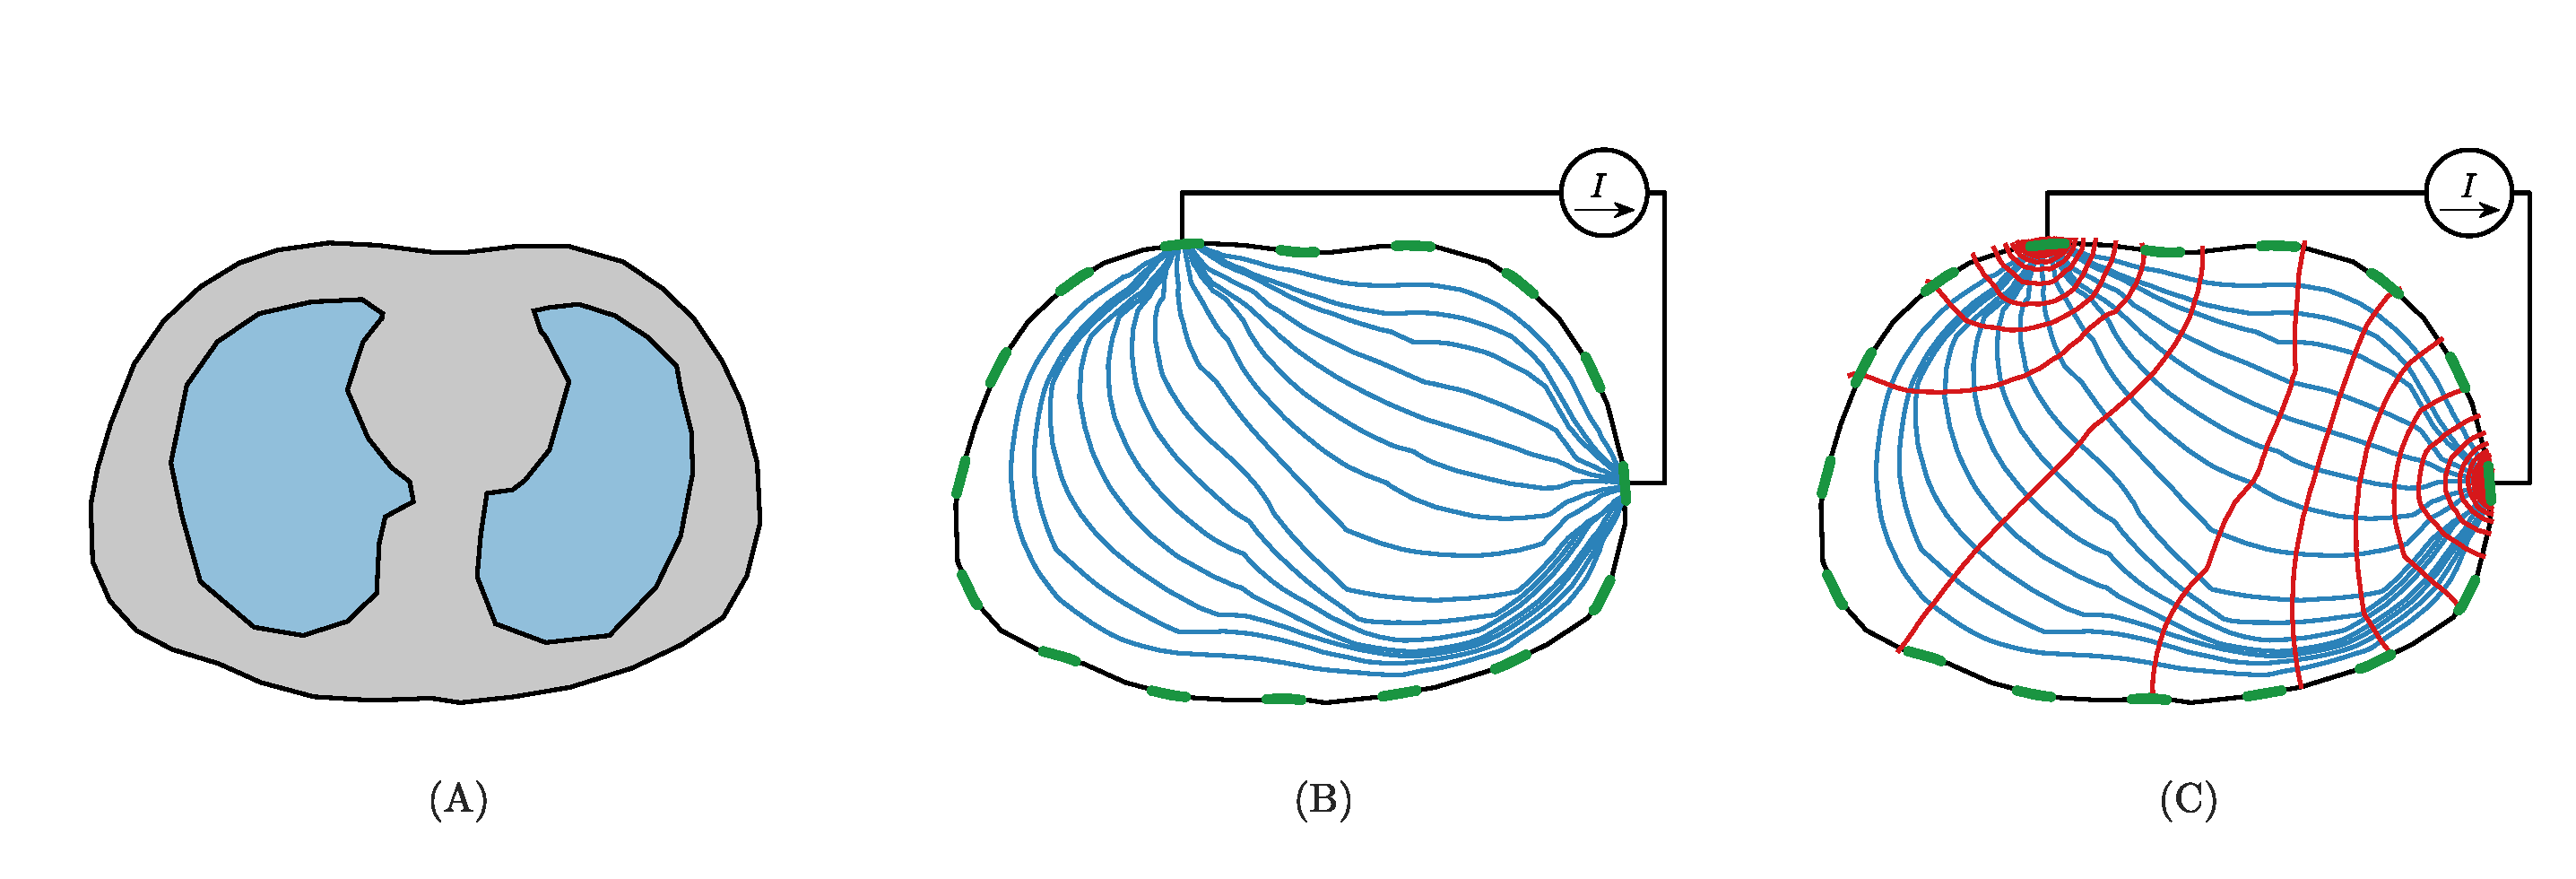
\includegraphics[width=\textwidth,trim={0 2cm 0 0},clip]{imgs/current_and_equipotential_lines.pdf}
	\end{figure}
	\vspace{2mm}
	Electrodes on the body surface are used to inject current and measure the resulting voltages. \\
	\vspace{0.5cm}
	Thoracic EIT typically images impedance changes due to the movement of fluid in the chest. \\
\end{frame}

\begin{frame}
	\frametitle{Background}
	\framesubtitle{Perfusion}
	{\Large What is \alert{perfusion}?} \\ \vspace{2mm}
	\begin{figure}[H]
		\centering
		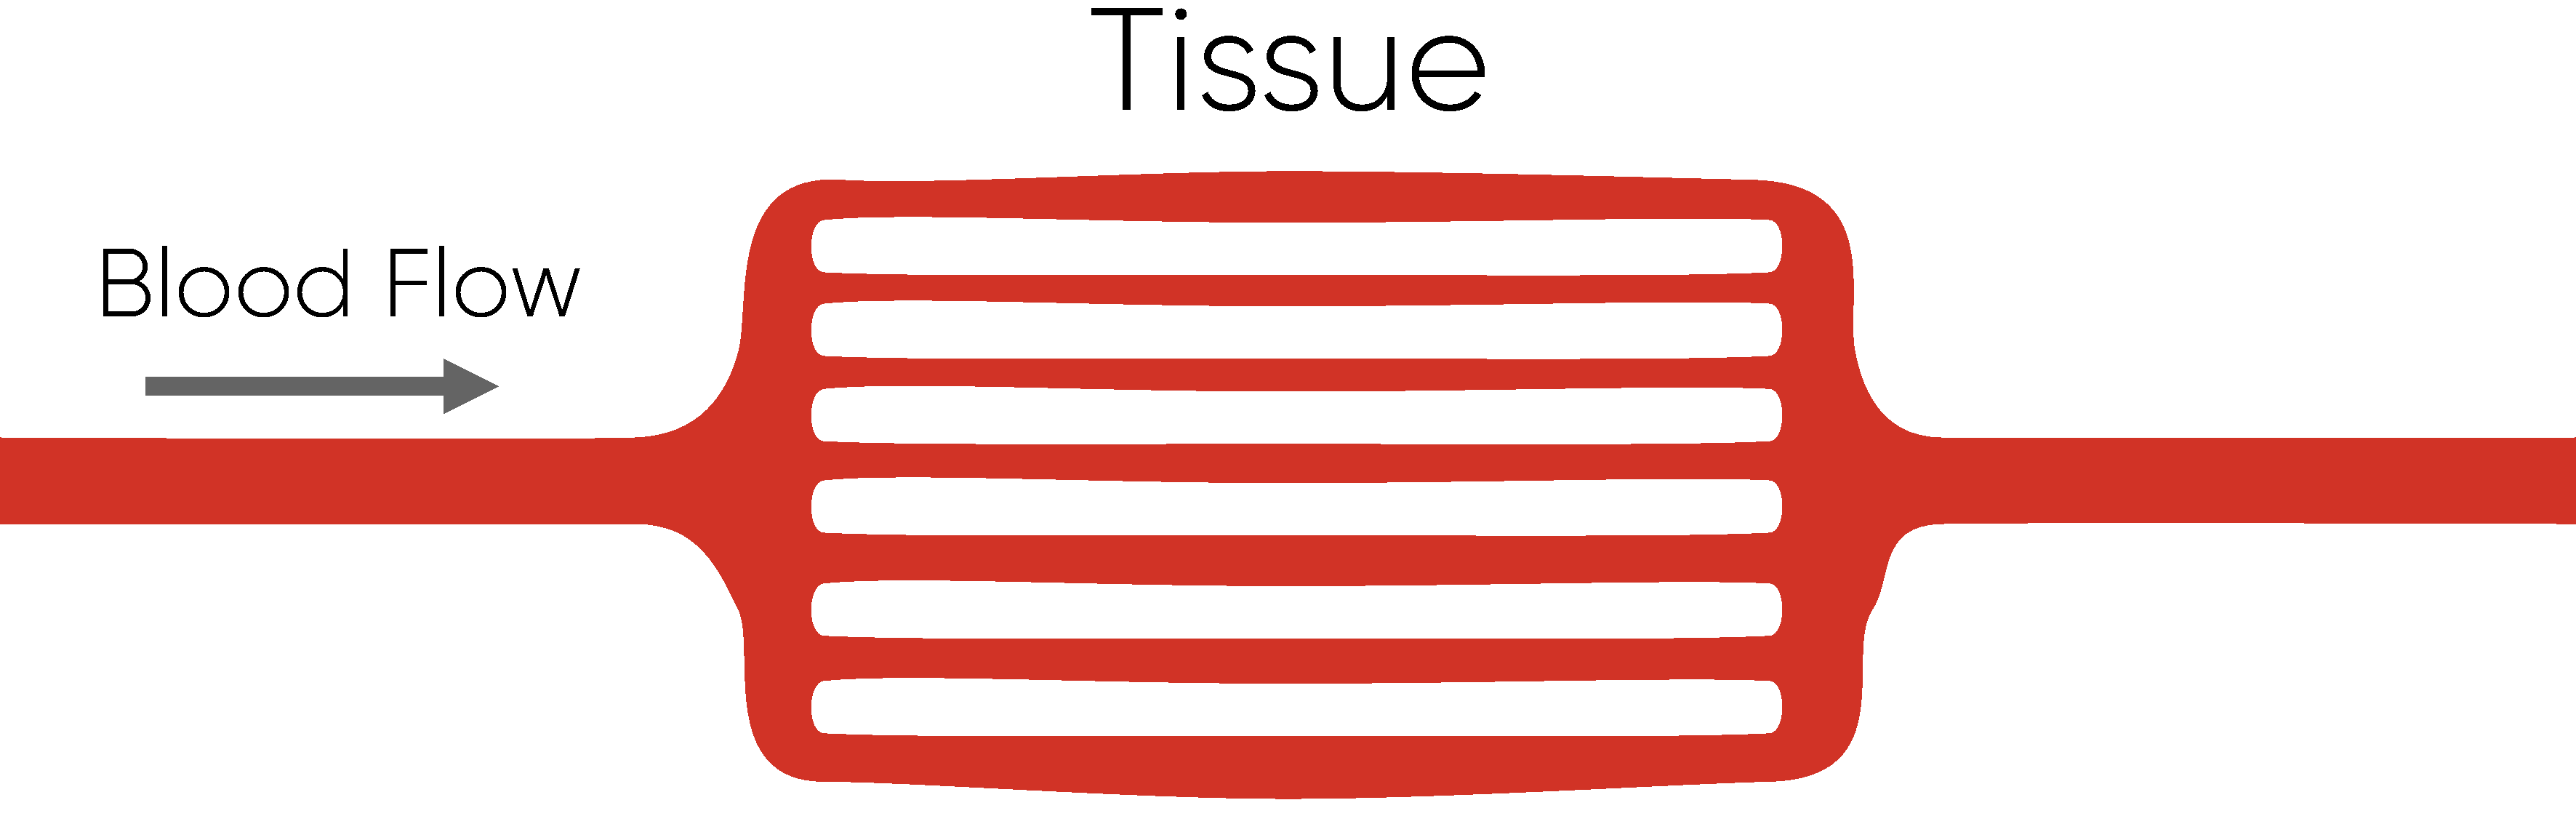
\includegraphics[width=\textwidth]{perfusion_sketch.pdf}
	\end{figure}

\end{frame}

\begin{frame}
	\frametitle{Background}
	\framesubtitle{EIT Measures of Perfusion}
	\begin{columns}[c]
		\begin{column}{0.5\textwidth}
			Blood perfuses into the tissue. \\ \vspace{2mm}
			\begin{figure}[H]
				\centering
				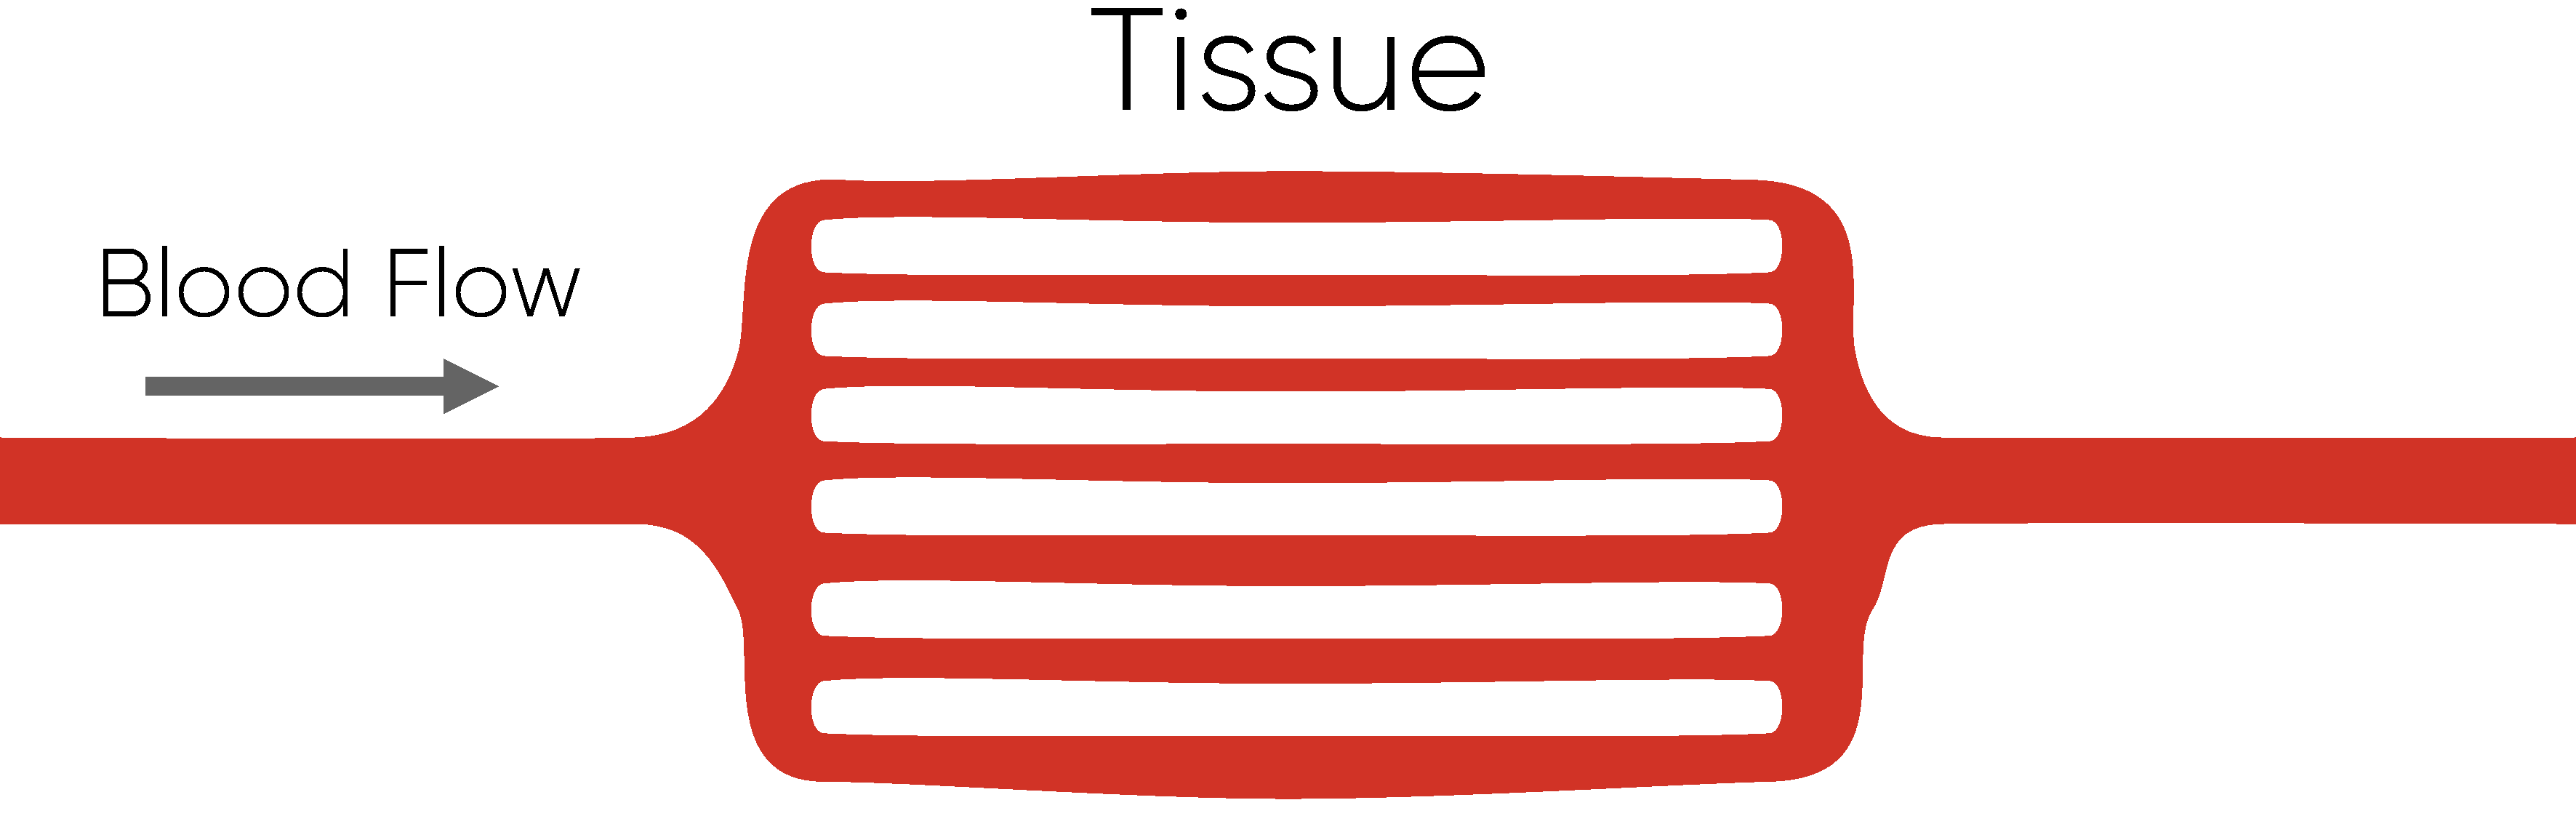
\includegraphics[width=\textwidth]{perfusion_sketch.pdf}
			\end{figure}
		\end{column}
		\begin{column}{0.5\textwidth}
			The perfusion signal can come from: \\ \vspace{2mm}
			\begin{itemize}
				\item Change in blood volume in the tissue
				\item Change in blood volume in vessels
				\item Physical deformation of structures due to movement
				\item Ballistic forces in the body 
				\item The orientation of red blood cells (very small change)
			\end{itemize}
		\end{column}
	\end{columns}
\end{frame}

\begin{frame}
	\frametitle{Background}
	\framesubtitle{EIT Perfusion Imaging}
\begin{columns}[c]
\begin{column}{0.5\textwidth}
	Compared to other techniques used to image perfusion EIT is: \\ \vspace{2mm}
	\begin{itemize}
		\item Fast 
		\item Does not use ionizing radiation 
		\item Can be used continuously 
		\item Cost efficient 
	\end{itemize}
\end{column}
\begin{column}{0.5\textwidth}
	Challenges of perfusion imaging with EIT: \\ \vspace{5mm}
	\begin{itemize}
		\item Unclear source of cardiac-frequency (cardiosynchronous) signal
		\item Low amplitude of cardiac-frequency signal
		\item Low sensitivity in the centre of a subject
	\end{itemize}
\end{column}
\end{columns}
\end{frame}

\begin{frame}
	\frametitle{Background}
	\framesubtitle{Challenges of EIT Perfusion Imaging}
\begin{columns}[c]
\begin{column}{0.5\textwidth}
\textbf{\large Not all perfusion results in a cardiac-frequency change}
\begin{itemize}
	\item e.g. Continuous flow
\end{itemize} %
\vspace{10mm}
\textbf{\large Non-perfusion effects can result in heart-frequency EIT signals}
\begin{itemize}
	\item e.g. Movement
\end{itemize}

\end{column}
\begin{column}{0.5\textwidth}
	Challenges of perfusion imaging with EIT: \\ \vspace{5mm}
	\begin{itemize}
		\item \textbf{Unclear source of cardiac-frequency (cardiosynchronous) signal}
		\item Low amplitude of cardiac-frequency signal
		\item Low sensitivity in the centre of a subject
	\end{itemize}
\end{column}
\end{columns}
\end{frame}

\begin{frame}
	\frametitle{Background}
	\framesubtitle{EIT Perfusion Imaging}
\begin{columns}[c]
\begin{column}{0.5\textwidth}
	\begin{figure}
		\centering
	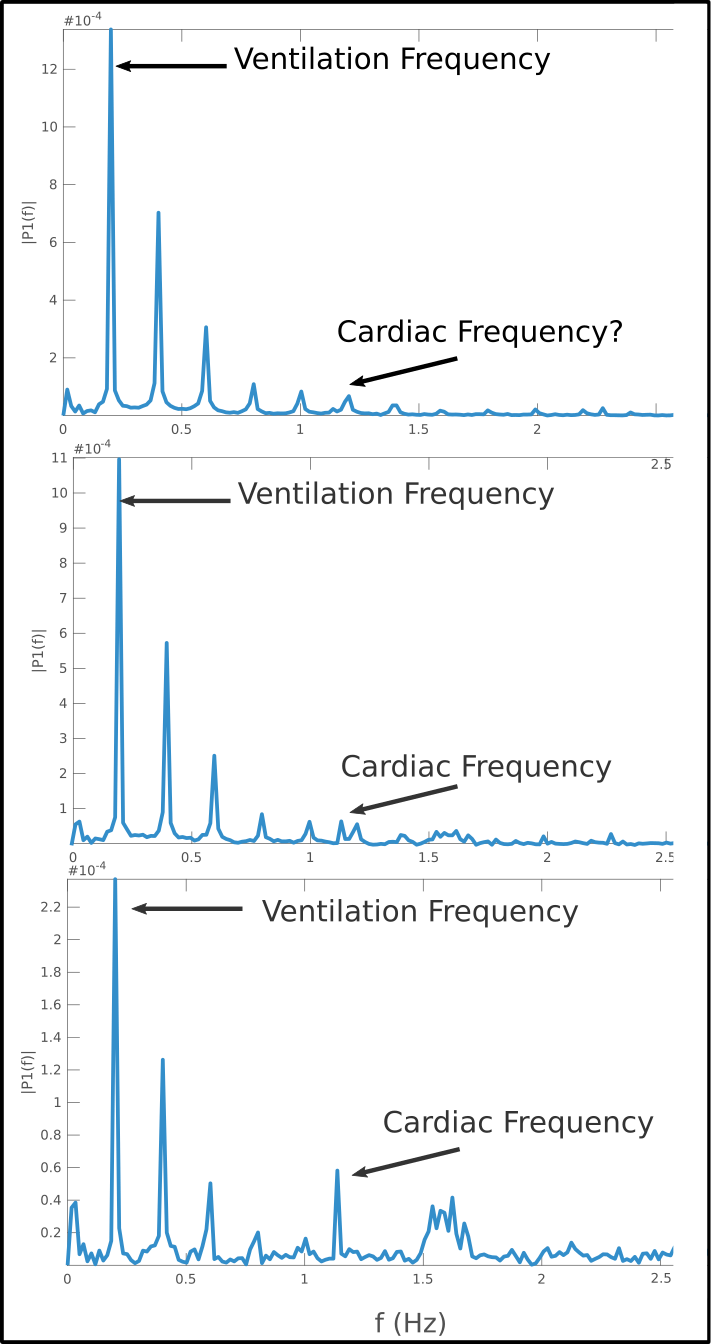
\includegraphics[width=\textwidth,trim={0.5cm 24cm 0.5cm 1cm},clip]{imgs/FFT_img.png}
	\end{figure}
	Example FFT of an EIT signal with only external electrodes (\alert{frequency in Hz}).
\end{column}
\begin{column}{0.5\textwidth}
	Challenges of perfusion imaging with EIT: \\ \vspace{5mm}
	\begin{itemize}
		\item Unclear source of cardiac-frequency (cardiosynchronous) signal
		\item \textbf{Low amplitude of cardiac-frequency signal}
		\item Low sensitivity in the centre of a subject
	\end{itemize}
\end{column}
\end{columns}
\end{frame}

\begin{frame}
	\frametitle{Background}
	\framesubtitle{EIT Perfusion Imaging}
\begin{columns}[c]
\begin{column}{0.5\textwidth}
	\begin{figure}
		\centering
	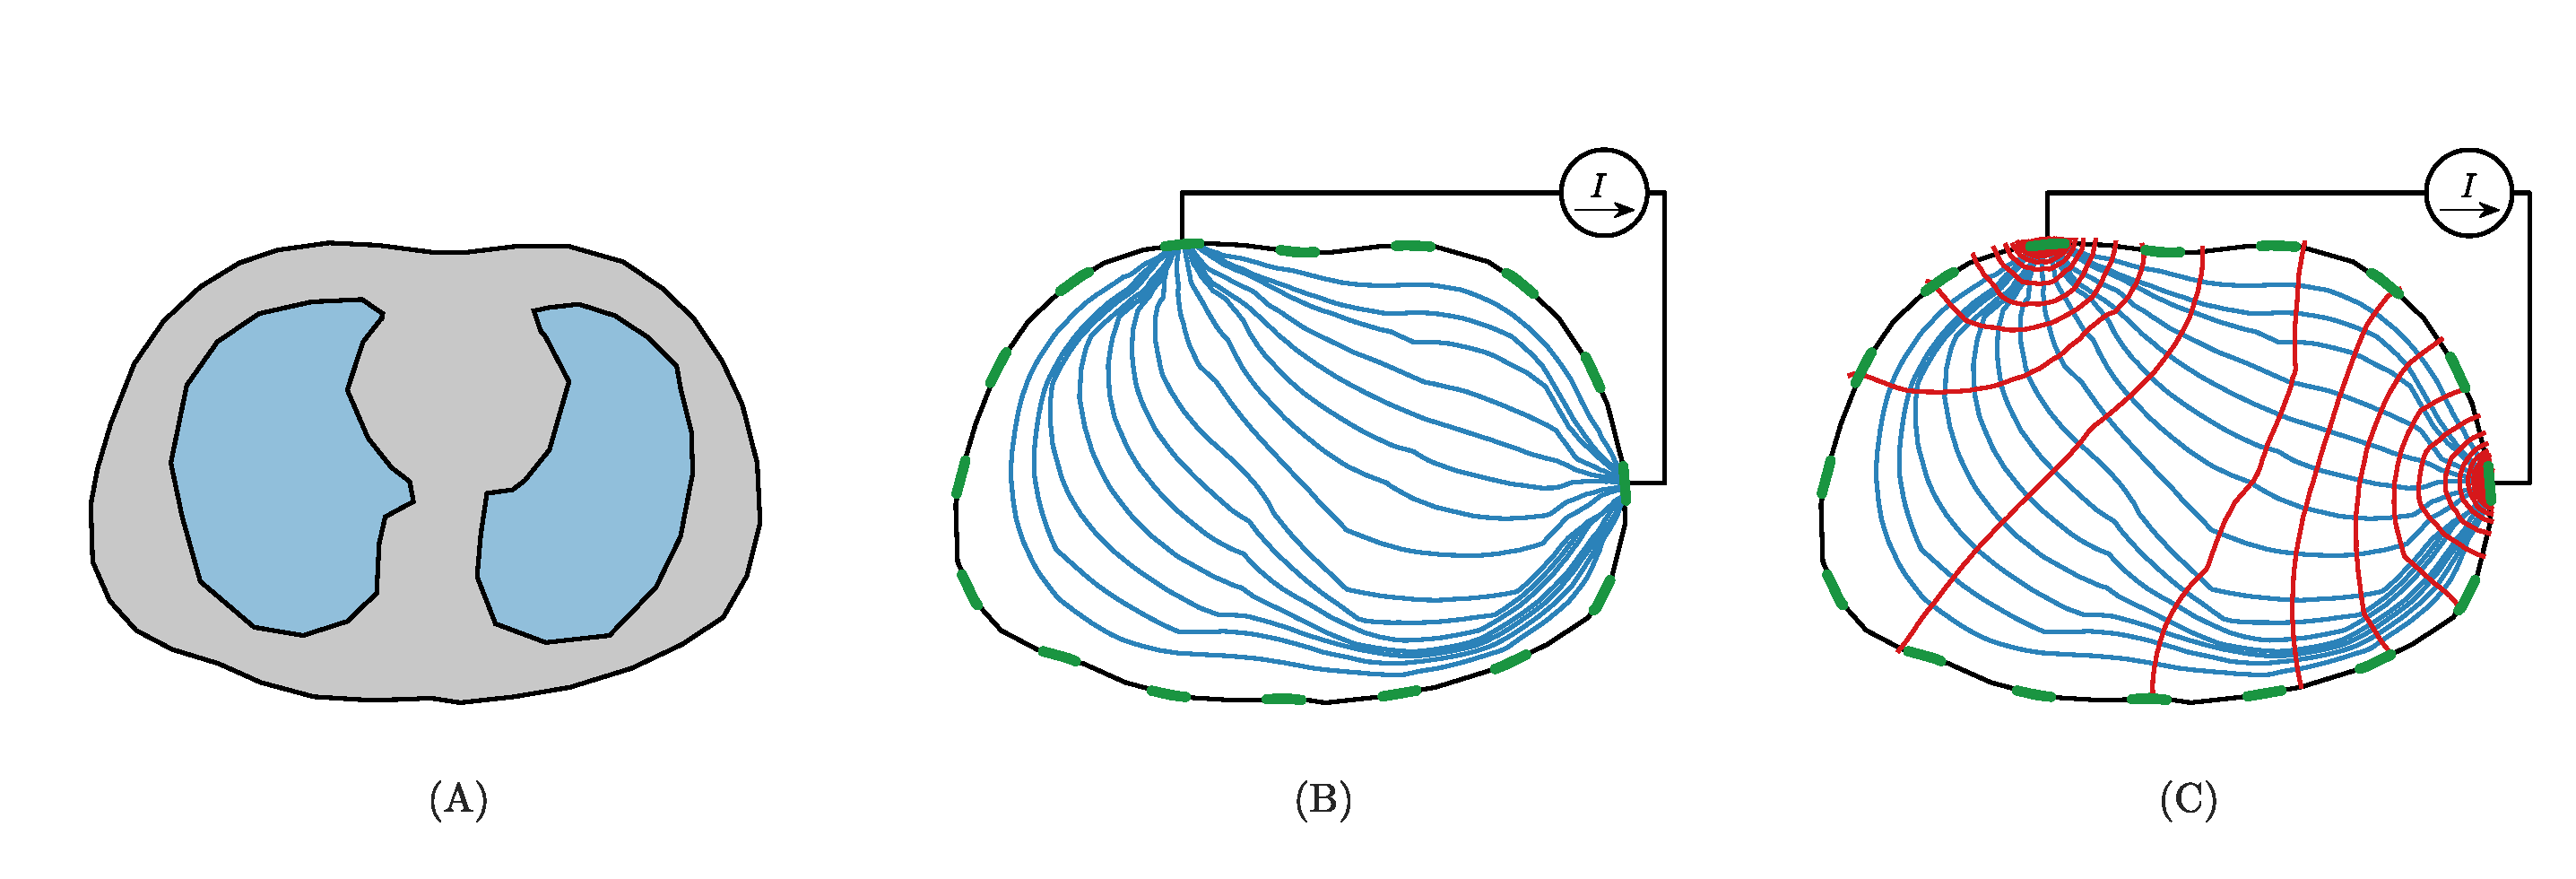
\includegraphics[width=\textwidth,trim={16cm 3cm 16cm 0},clip]{imgs/current_and_equipotential_lines.pdf}
	\end{figure}
	\alert{Sensitivity} is proportional to \alert{current density}.
\end{column}
\begin{column}{0.5\textwidth}
	Challenges of perfusion imaging with EIT: \\ \vspace{5mm}
	\begin{itemize}
		\item Unclear source of cardiac-frequency (cardiosynchronous) signal
		\item Low amplitude of cardiac-frequency signal
		\item \textbf{Low sensitivity in the centre of a subject}
	\end{itemize}
\end{column}
\end{columns}
\end{frame}

\begin{frame}
	\frametitle{Background}
	\framesubtitle{Current State of EIT Perfusion Imaging}
	\begin{columns}[c]
		\begin{column}{0.33\textwidth}
			\alert{\large Bolus Injection} \\ \vspace{2mm}
			\begin{itemize}
				\item A conductive contrast agent is injected
				\item The transit of the conductive contrast agent is imaged
				\vspace{3mm}
				\item Occurs during apnoea
				\item Saline solution is typically used 
			\end{itemize}
		\end{column}
		\begin{column}{0.33\textwidth}
			\alert{\large Frequency Filtering} \\ \vspace{2mm}
			\begin{itemize}
				\item The signal at the cardiac frequency is isolated
				\item An image of activity at the cardiac frequency is generated
				\item Can be done during either ventilation or apnoea
			\end{itemize}
		\end{column}
		\begin{column}{0.33\textwidth}
			\alert{\large Ensemble Averaging} \\ \vspace{2mm}
			\begin{itemize}
				\item Many heartbeats are averaged together 
				\item An image of the impedance change over the averaged heartbeat is generated
				\item Can be done during either ventilation or apnoea
			\end{itemize}
		\end{column}
		\end{columns}
\end{frame}

\begin{frame}
	\frametitle{Background}
	\framesubtitle{Shortcomings of EIT Perfusion Measures}
	\begin{columns}[c]
		\begin{column}{0.5\textwidth}
			\begin{itemize}
				\item Bolus-based measures cannot be used continuously and are invasive
				\item Filtering-based methods have low sensitivity to cardiosynchronous activity
				\item Low internal sensitivity 
			\end{itemize}
		\end{column}
		\begin{column}{0.5\textwidth}
			How can measures of \alert{perfusion} be improved? 
			\begin{enumerate}
				\item Investigate the source of perfusion and cardiosynchronous EIT signals
				\item Increase sensitivity near where perfusion is measured
			\end{enumerate}
		\end{column}
		\end{columns}	
\end{frame}

\begin{frame}
	\frametitle{Thesis Goals}
	\begin{figure}
		\centering
	%\begin{tikzpicture}
	%<code goes here>
	%\end{tikzpicture}
	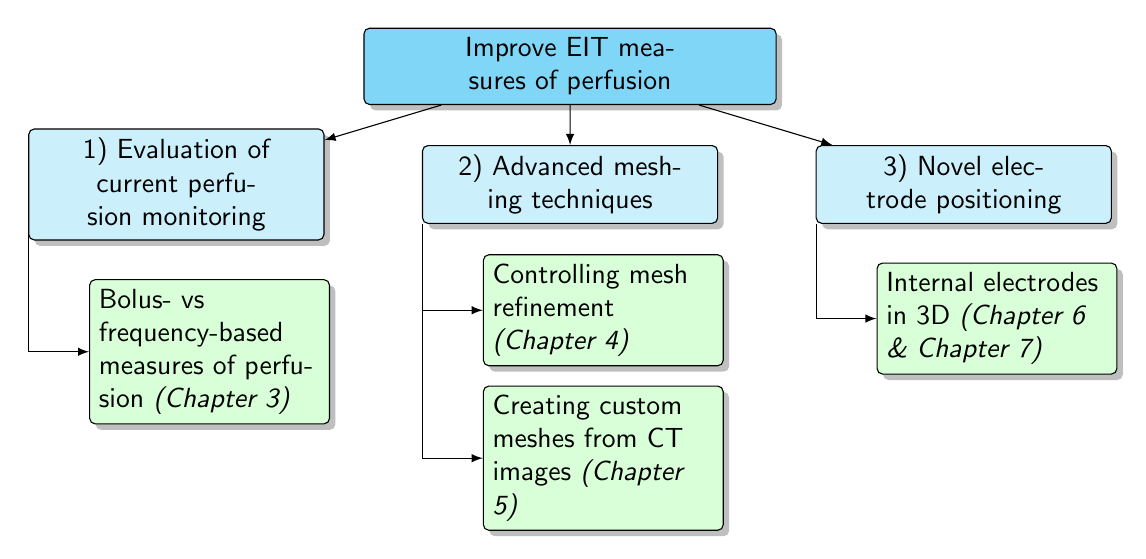
\begin{tikzpicture}[
	  level 1/.style={sibling distance=50mm},
	  edge from parent/.style={->,draw},
	  >=latex]
	
	% root of the the initial tree, level 1
	\node[root] {Improve EIT measures of perfusion}
	% The first level, as children of the initial tree
	  child {node[level 2] (c1) {1) Evaluation of current perfusion monitoring}}
	  child {node[level 2] (c2) {2) Advanced meshing techniques}}
	  child {node[level 2] (c3) {3) Novel electrode positioning}};
	
	% The second level, relatively positioned nodes
	\begin{scope}[every node/.style={level 3}]
	\node [below of = c1, xshift=12pt, yshift=-32pt] (c11) {Bolus- vs 
	frequency-based measures of perfusion \emph{(Chapter 3)}}; 
	
	\node [below of = c2, xshift=12pt, yshift=-17pt] (c21) 
	{Controlling mesh refinement\\ \emph{(Chapter 4)}};
	\node [below of = c21, yshift=-25pt] (c22) 
	{Creating custom meshes from CT images \emph{(Chapter 5)}};
	\node [below of = c3, xshift=12pt, yshift=-20pt] (c31) 
	{Internal electrodes in 3D \emph{(Chapter 6 \& Chapter 7)}};
	\end{scope}
	
	% lines from each level 1 node to every one of its "children"
	\foreach \value in {1}
	  \draw[->] (c1.195) |- (c1\value.west);
	
	\foreach \value in {1,2}
	  \draw[->] (c2.195) |- (c2\value.west);
	
	\foreach \value in {1}
	  \draw[->] (c3.195) |- (c3\value.west);
	
	\end{tikzpicture}
\end{figure}
\end{frame}

\begin{frame}
	\frametitle{Contributions}    
	\begin{columns}[c]
		\begin{column}{0.5\textwidth}
			\begin{enumerate}
				\item A mesh analysis technique to reduce error in sensitivity calculations on 
				cylindrical meshes (\alert{Chapter 4}). \\ \vspace{4mm}
				\item A tool to generate custom meshes of exterior and lung boundaries from CT images
				(\alert{Chapter 5}).
			\end{enumerate}
		\end{column}
		\begin{column}{0.5\textwidth}
			\begin{enumerate}
				\setcounter{enumi}{2}
				\item An analysis of 3D electrode placements with internal electrodes on internal 
				sensitivity (\alert{Chapter 6}). \\ \vspace{4mm}
				\item A method to reconstruct images using internal electrode measurements in the
				presence of movement (\alert{Chapter 7}).
			\end{enumerate}
		\end{column}
	\end{columns}
\end{frame}

\begin{frame}
	\frametitle{Chapter 3: Bolus- and Frequency-Based Perfusion}
	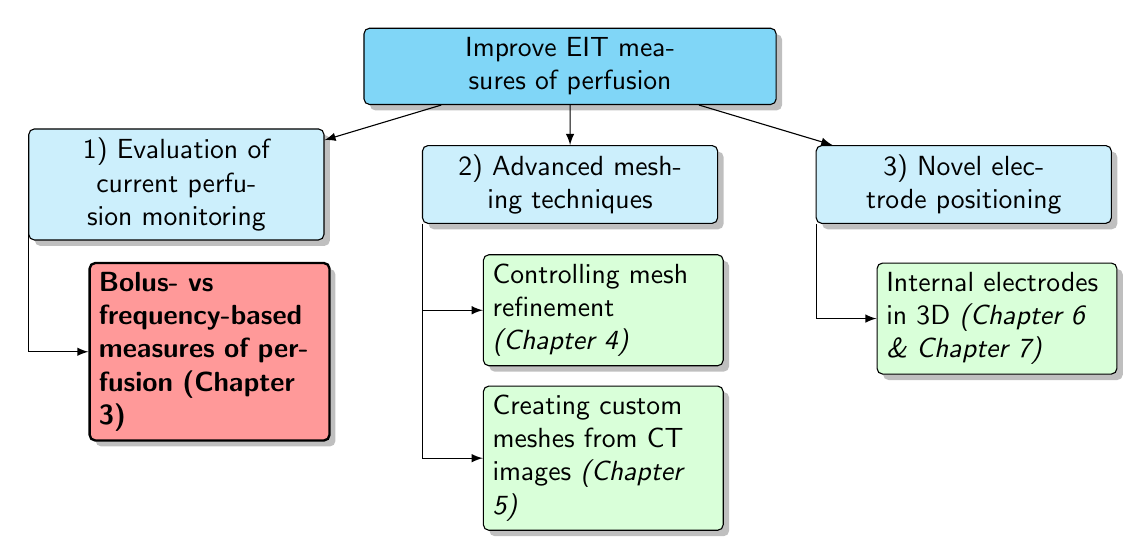
\begin{tikzpicture}[
		level 1/.style={sibling distance=50mm},
		edge from parent/.style={->,draw},
		>=latex]
	  
	  % root of the the initial tree, level 1
	  \node[root] {Improve EIT measures of perfusion}
	  % The first level, as children of the initial tree
		child {node[level 2] (c1) {1) Evaluation of current perfusion monitoring}}
		child {node[level 2] (c2) {2) Advanced meshing techniques}}
		child {node[level 2] (c3) {3) Novel electrode positioning}};
	  
	  % The second level, relatively positioned nodes
	  \begin{scope}[every node/.style={level 3}]
	  \node [below of = c1, xshift=12pt, yshift=-32pt, fill=red!40 ,line width=0.3mm] (c11) {\textbf{Bolus- vs 
	  frequency-based measures of perfusion \emph{(Chapter 3)}}}; 
	  
	  \node [below of = c2, xshift=12pt, yshift=-17pt] (c21) 
	  {Controlling mesh refinement\\ \emph{(Chapter 4)}};
	  \node [below of = c21, yshift=-25pt] (c22) 
	  {Creating custom meshes from CT images \emph{(Chapter 5)}};
	  \node [below of = c3, xshift=12pt, yshift=-20pt] (c31) 
	  {Internal electrodes in 3D \emph{(Chapter 6 \& Chapter 7)}};
	  \end{scope}
	  
	  % lines from each level 1 node to every one of its "children"
	  \foreach \value in {1}
		\draw[->] (c1.195) |- (c1\value.west);
	  
	  \foreach \value in {1,2}
		\draw[->] (c2.195) |- (c2\value.west);
	  
	  \foreach \value in {1}
		\draw[->] (c3.195) |- (c3\value.west);
	  
	  \end{tikzpicture}
\end{frame}

\begin{frame}
	\vspace{5mm}
	\frametitle{Chapter 3: Bolus- and Frequency-Based Perfusion}
	\framesubtitle{Introduction}
	\begin{columns}[c]
	\begin{column}{0.5\textwidth}
		There are \alert{three common techniques} to measure perfusion with EIT. \\ \vspace{2mm}
		\begin{enumerate}
			\item Bolus injection 
			\item Frequency filtering
			\item Ensemble averaging
		\end{enumerate}
	\end{column}
	\begin{column}{0.5\textwidth}
		\textbf{Goals}
		\begin{itemize}
			\item Compare different measures of perfusion.
			\item Investigate the source of cardiosynchronous EIT signals. 
		\end{itemize}
	\end{column}
	\end{columns}
\end{frame}

\begin{frame}
	\frametitle{Chapter 3: Bolus- and Frequency-Based Perfusion}
	\framesubtitle{Methods}
	\begin{columns}[c]
		\begin{column}{0.5\textwidth}
	\begin{figure}
		\centering
	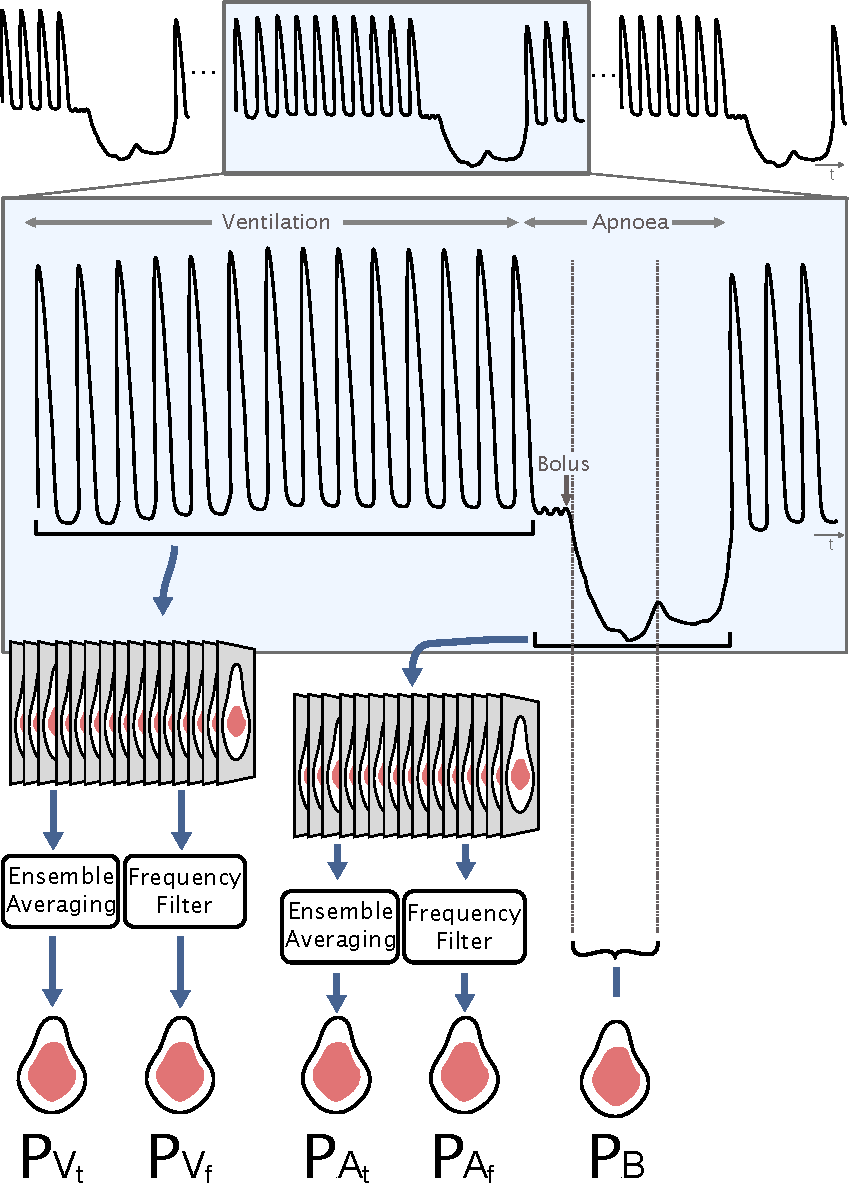
\includegraphics[width=0.9\textwidth,trim={0 0 0 3.35cm},clip]{imgs/fig-methodsOverview.pdf}
	\end{figure}
\end{column}
\begin{column}{0.5\textwidth}
	\begin{itemize}
		\item Data segment with ventilation and apnoea segments
		\item 7 animals, 4 postures (supine, left side, right side, prone)
		\item Frequency filtering ($P_V$) and ensemble averaging ($P_A$) methods used during both
		ventilation and apnoea
		\item Compared to a bolus injection during apnoea
	\end{itemize}
\end{column}
\end{columns}
\end{frame}

\begin{frame}
	\frametitle{Chapter 3: Bolus- and Frequency-Based Perfusion}
	\framesubtitle{Results}
	\begin{figure}
		\centering
	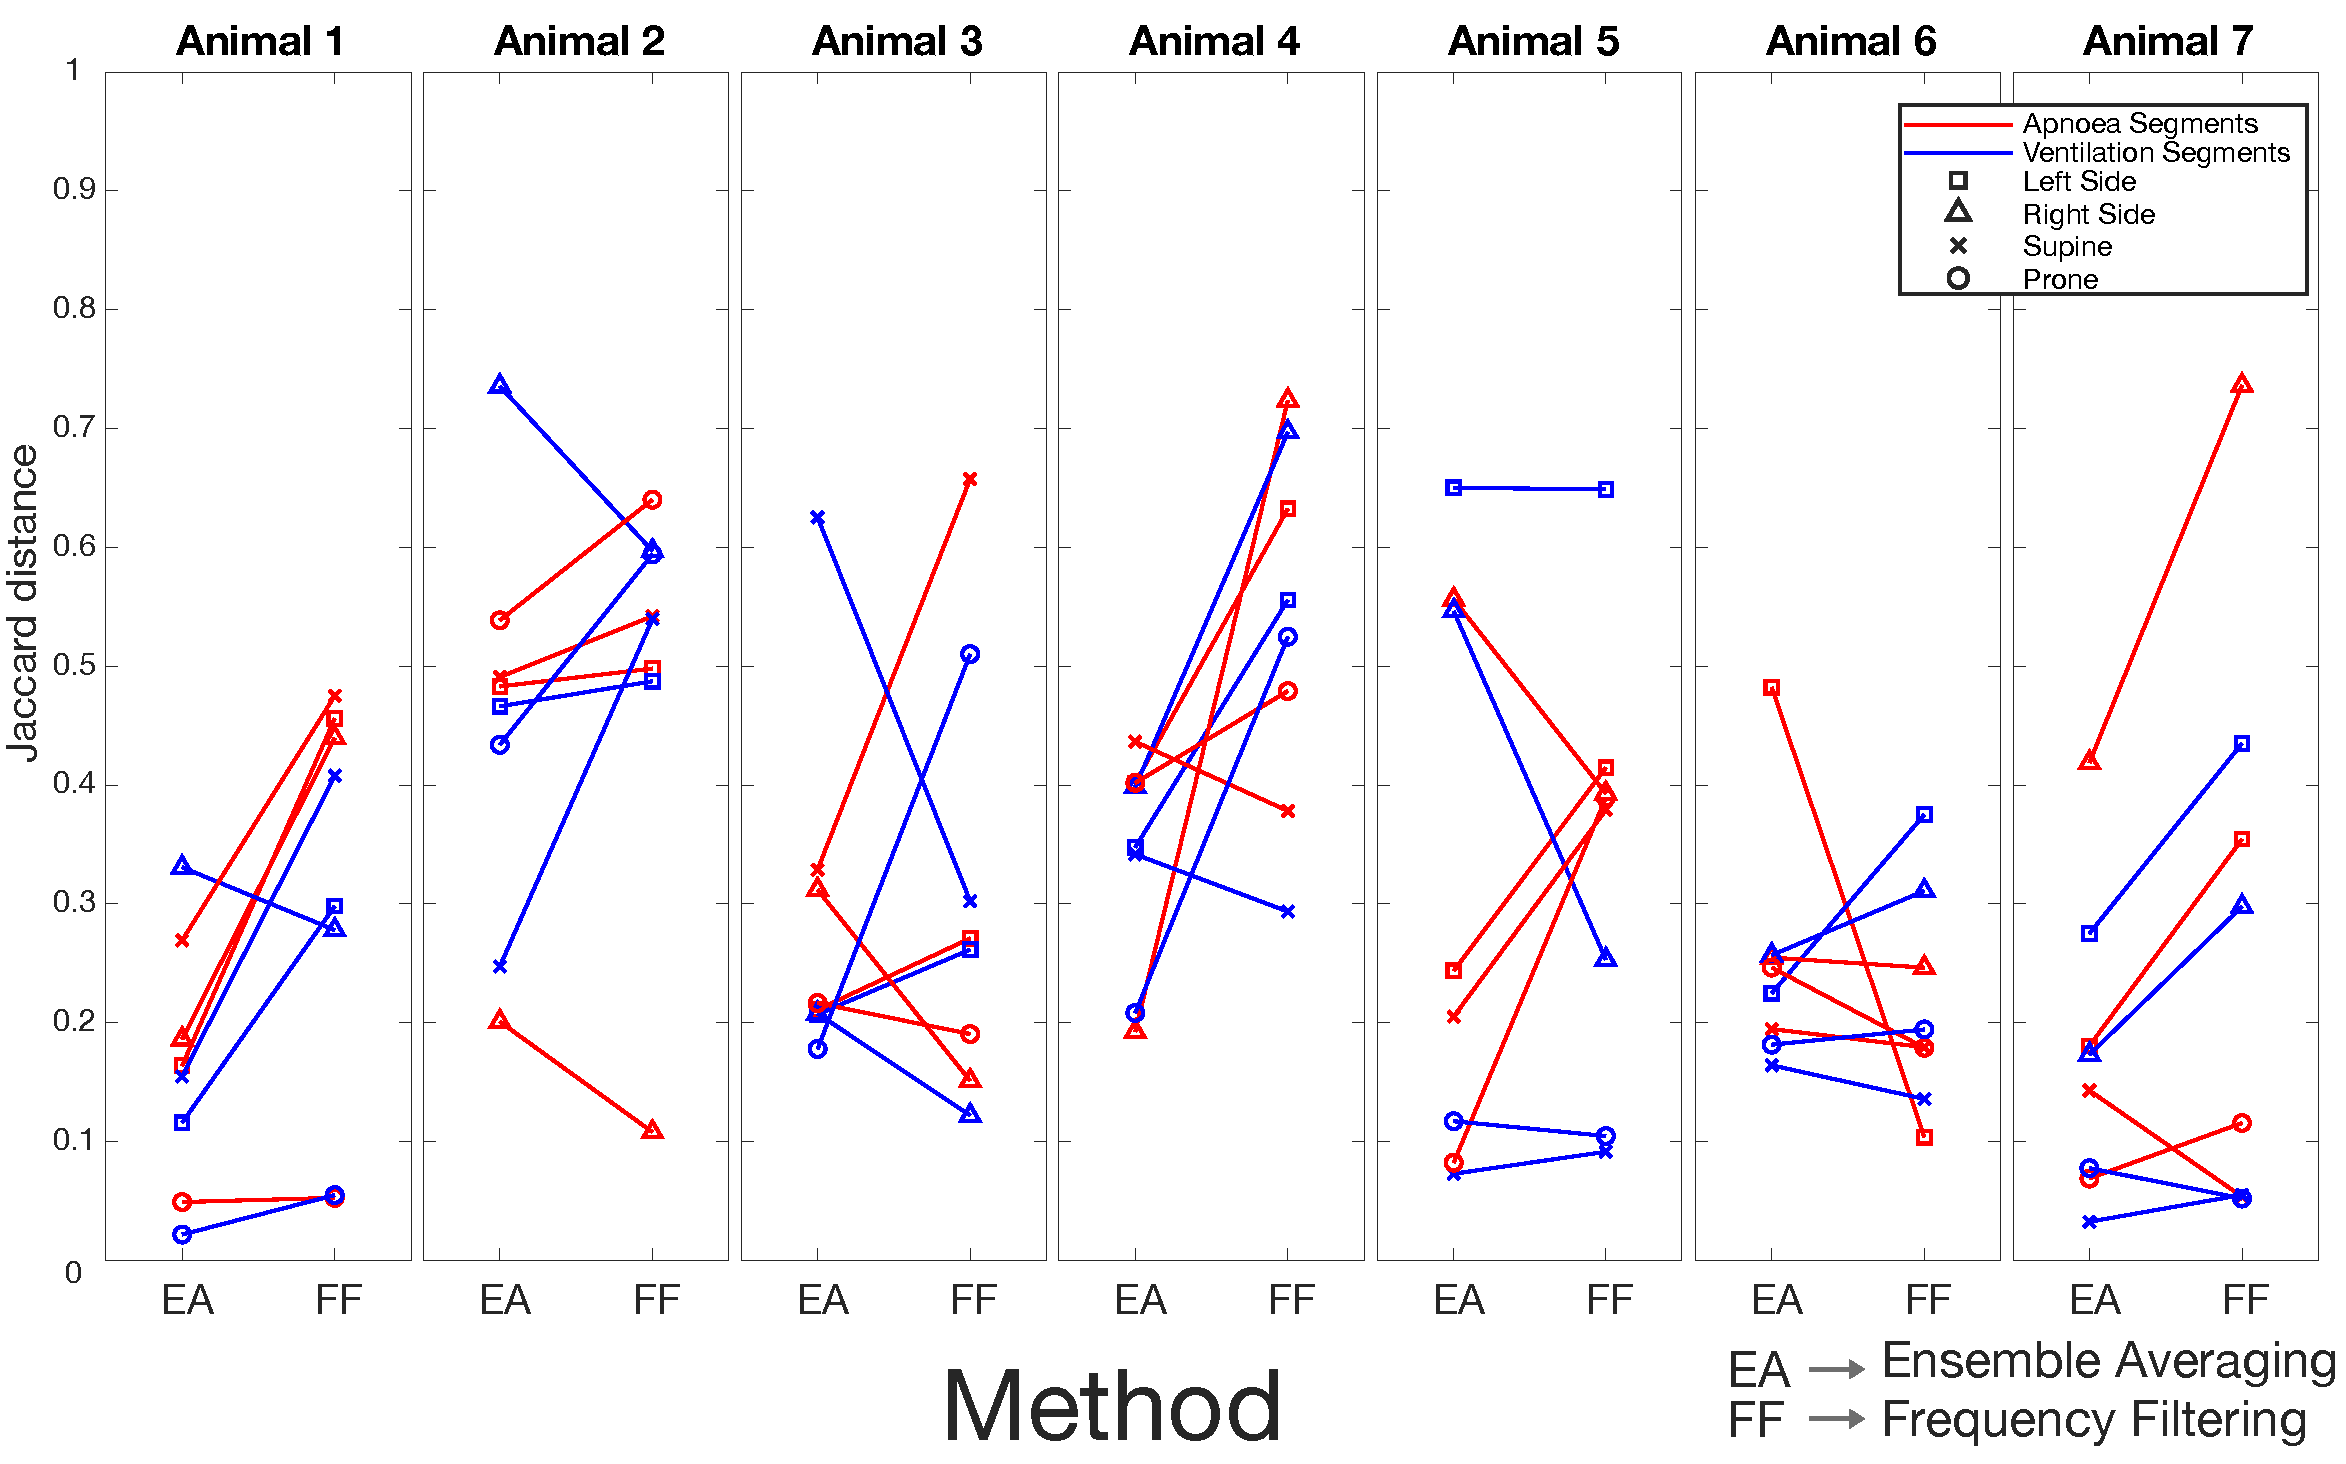
\includegraphics[width=0.9\textwidth]{imgs/fig-resultsJaccard.pdf}
	\end{figure}
\end{frame}

\begin{frame}
	\frametitle{Chapter 3: Bolus- and Frequency-Based Perfusion}
	\framesubtitle{Results}
	\begin{columns}[c]
		\begin{column}{0.5\textwidth}
	\begin{figure}
		\centering
	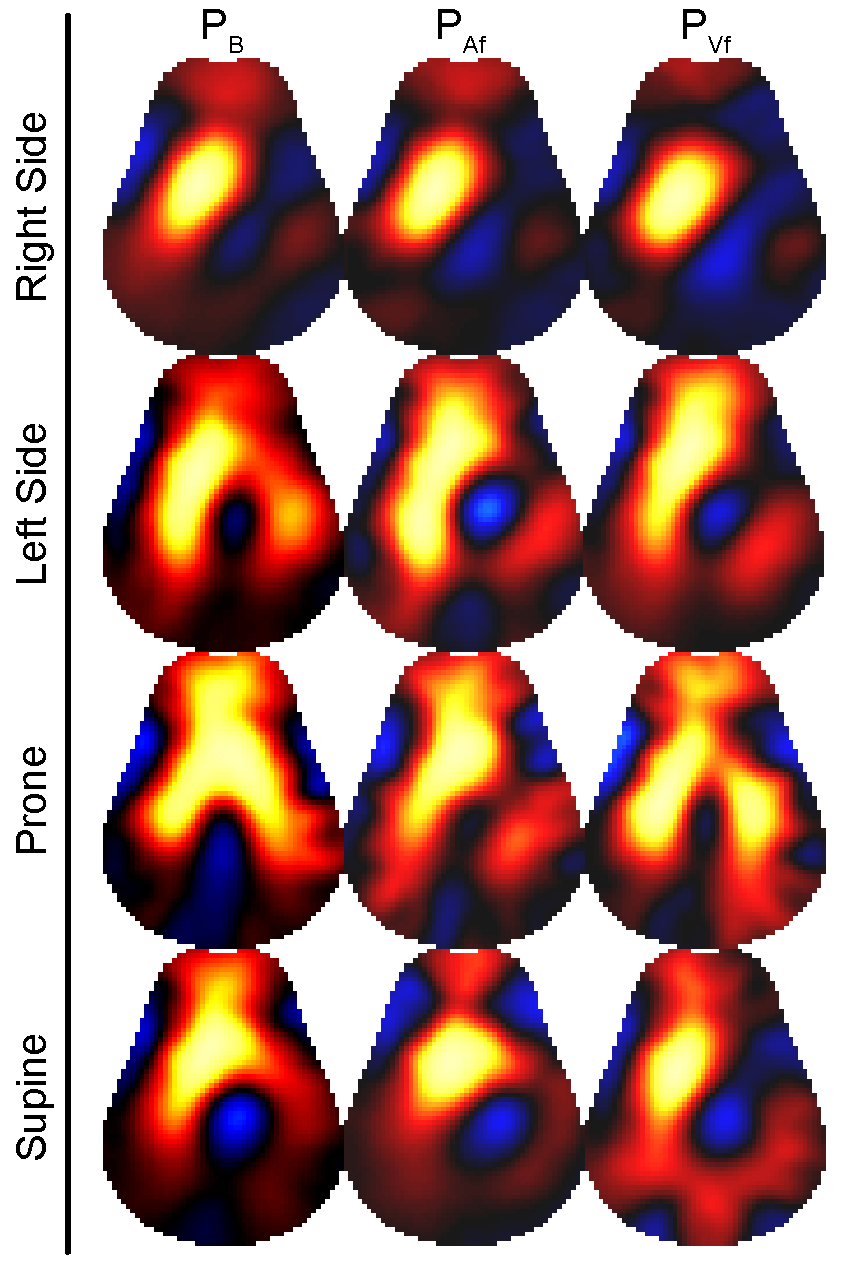
\includegraphics[width=0.7\textwidth,trim={0 0 0 0cm},clip]{imgs/fig-discussionSample.pdf}
	\end{figure}
\end{column}
\begin{column}{0.5\textwidth}
	\begin{itemize}
		\item Frequency filtering corresponds better to the bolus injection compared to ensemble averaging
		\item Challenging to isolate the lung regions
		\item Large contribution from the heart in the perfusion estimate
	\end{itemize}
\end{column}
\end{columns}
\end{frame}

\begin{frame}
	\frametitle{Chapter 4: FEM Mesh Refinement for 3D EIT}
	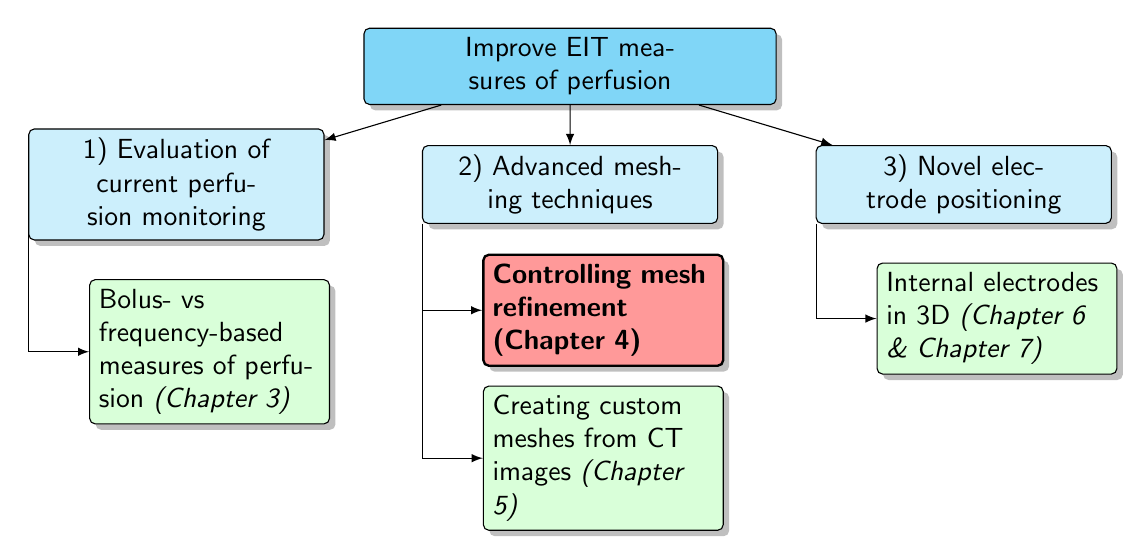
\begin{tikzpicture}[
		level 1/.style={sibling distance=50mm},
		edge from parent/.style={->,draw},
		>=latex]
	  
	  % root of the the initial tree, level 1
	  \node[root] {Improve EIT measures of perfusion}
	  % The first level, as children of the initial tree
		child {node[level 2] (c1) {1) Evaluation of current perfusion monitoring}}
		child {node[level 2] (c2) {2) Advanced meshing techniques}}
		child {node[level 2] (c3) {3) Novel electrode positioning}};
	  
	  % The second level, relatively positioned nodes
	  \begin{scope}[every node/.style={level 3}]
	  \node [below of = c1, xshift=12pt, yshift=-32pt] (c11) {Bolus- vs 
	  frequency-based measures of perfusion \emph{(Chapter 3)}}; 
	  
	  \node [below of = c2, xshift=12pt, yshift=-17pt, fill=red!40 ,line width=0.3mm] (c21) 
	  {\textbf{Controlling mesh refinement\\ \emph{(Chapter 4)}}};
	  \node [below of = c21, yshift=-25pt] (c22) 
	  {Creating custom meshes from CT images \emph{(Chapter 5)}};
	  \node [below of = c3, xshift=12pt, yshift=-20pt] (c31) 
	  {Internal electrodes in 3D \emph{(Chapter 6 \& Chapter 7)}};
	  \end{scope}
	  
	  % lines from each level 1 node to every one of its "children"
	  \foreach \value in {1}
		\draw[->] (c1.195) |- (c1\value.west);
	  
	  \foreach \value in {1,2}
		\draw[->] (c2.195) |- (c2\value.west);
	  
	  \foreach \value in {1}
		\draw[->] (c3.195) |- (c3\value.west);
	  
	  \end{tikzpicture}
\end{frame}

\begin{frame}
	\frametitle{Chapter 4: FEM Mesh Refinement for 3D EIT}
	\framesubtitle{Introduction \& Methods}
	What distribution of nodes minimizes error in the sensitivity calculation?
	\begin{figure}
		\centering
	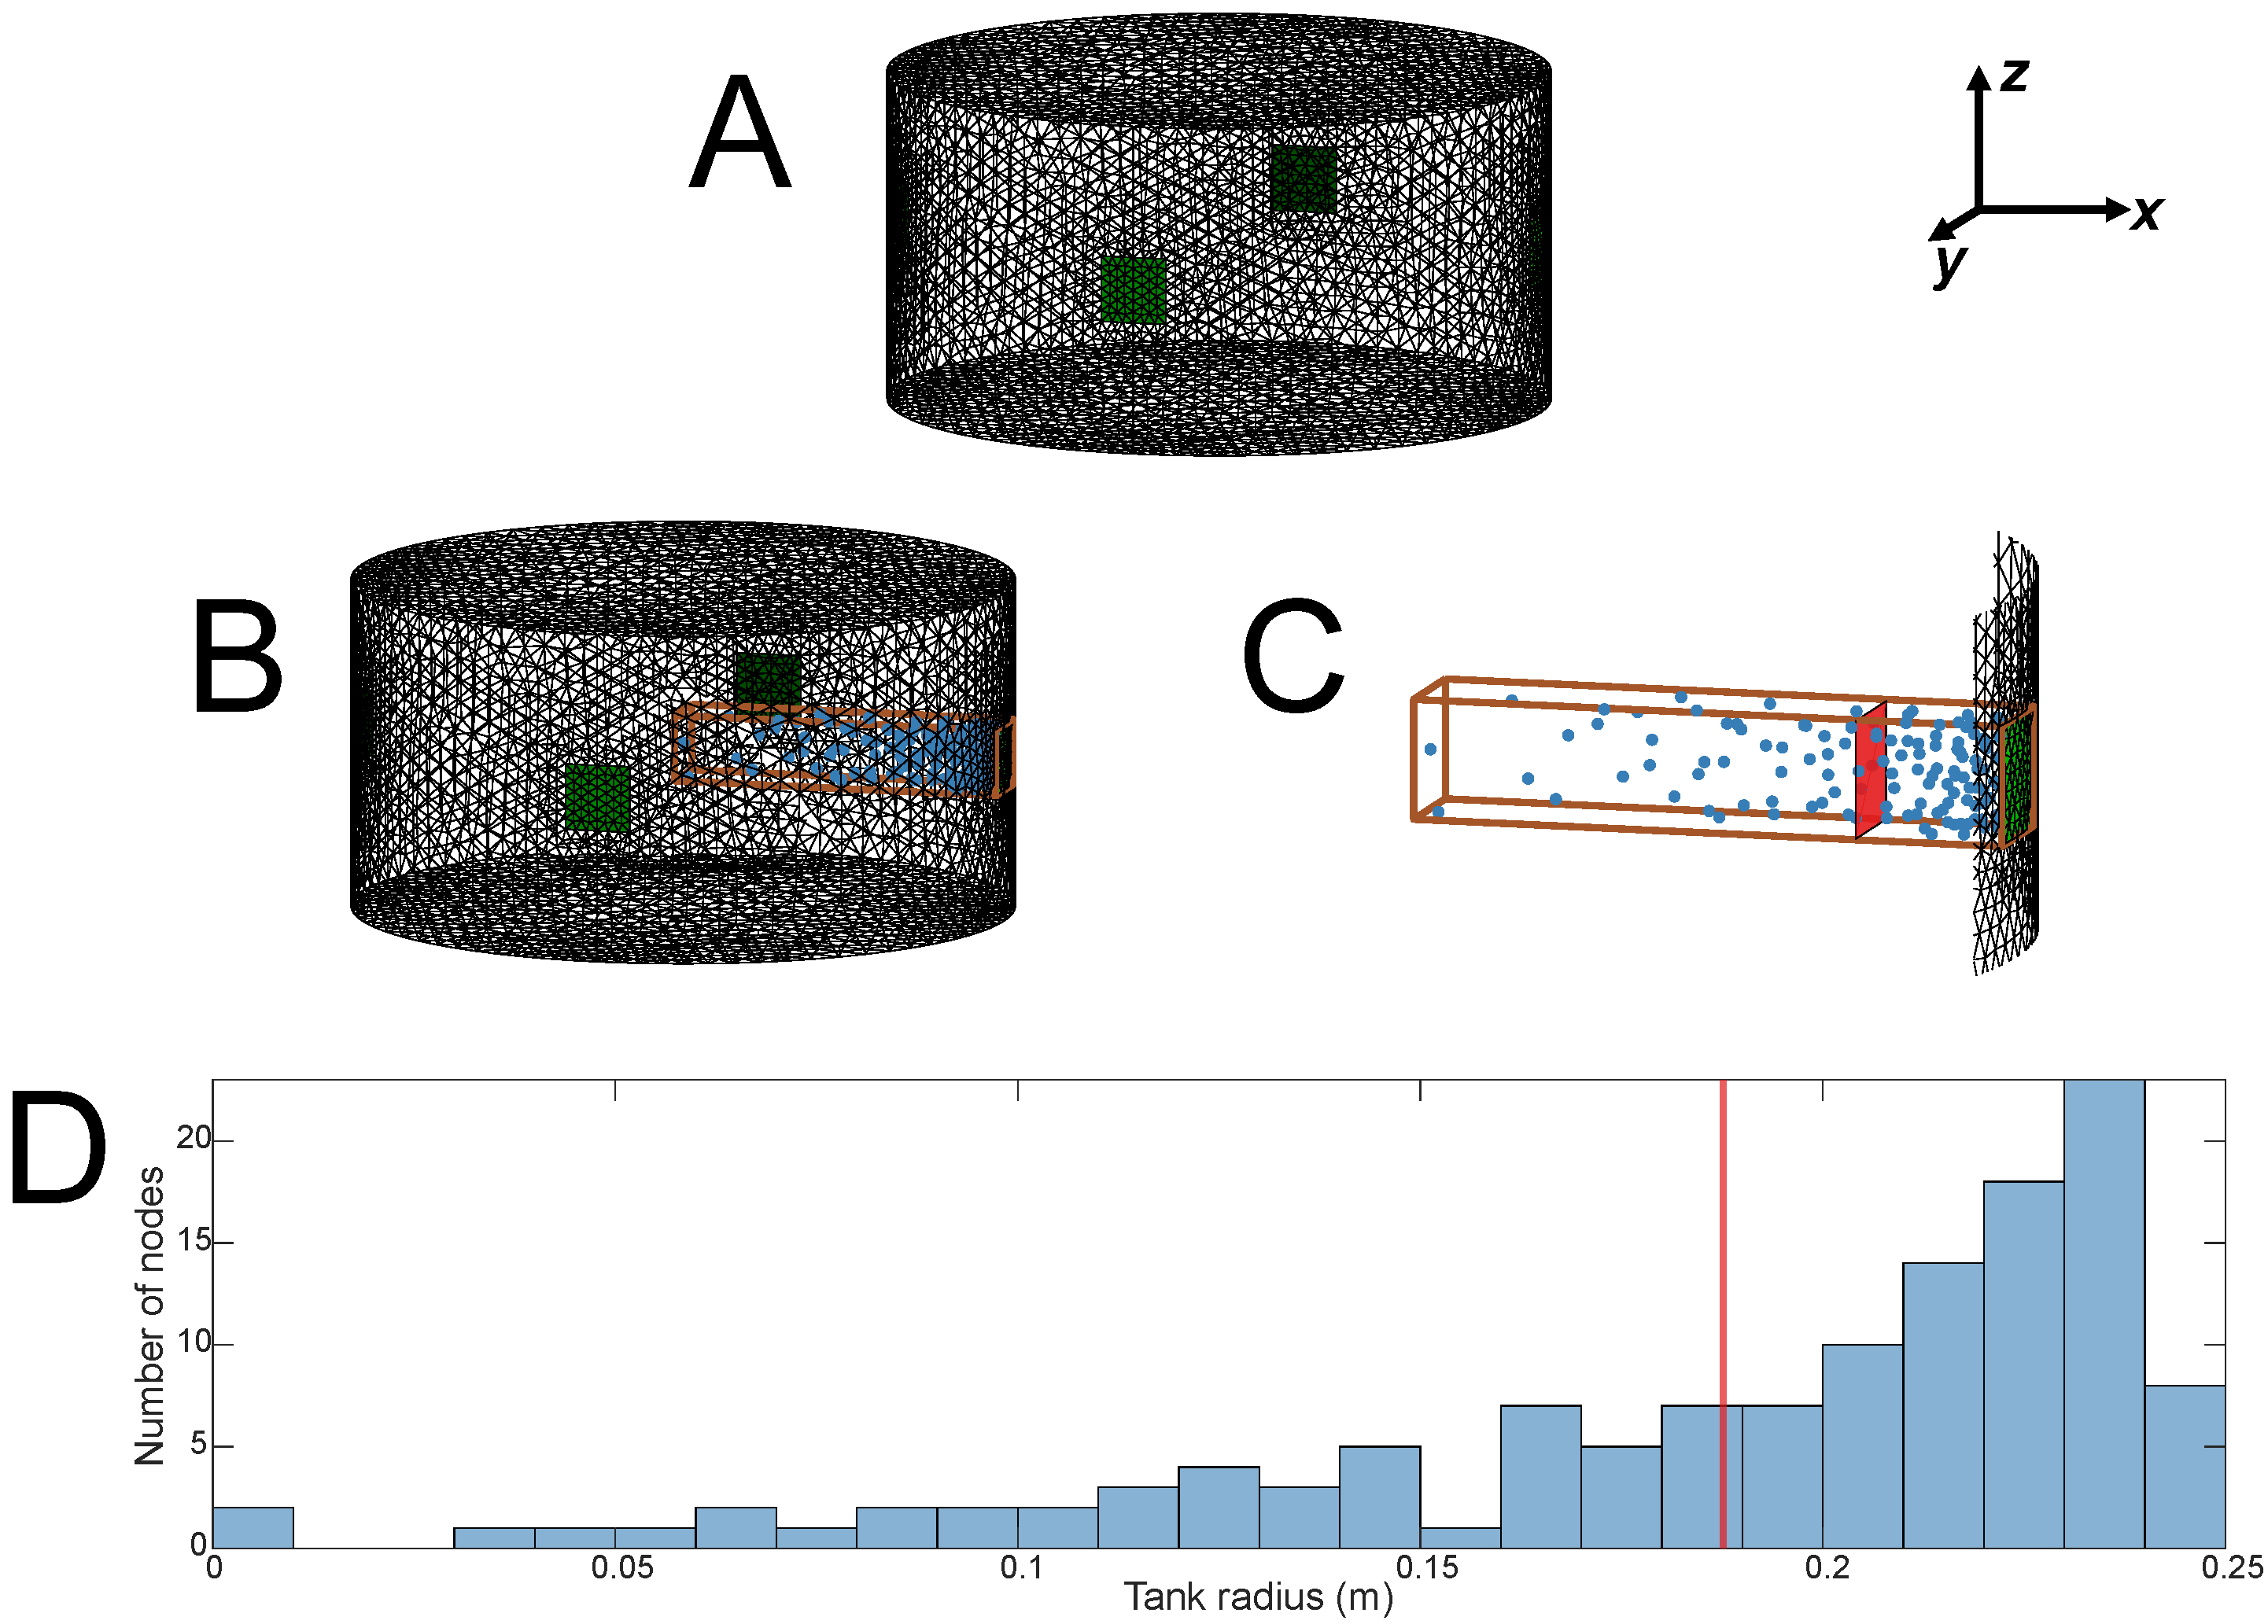
\includegraphics[width=0.9\textwidth,trim={0 0cm 0 10cm},clip]{balance_methods.pdf}
	\end{figure}
\end{frame}

\begin{frame}
	\frametitle{Chapter 4: FEM Mesh Refinement for 3D EIT}
	\framesubtitle{Results}
	\begin{columns}[c]
		\begin{column}{0.47\textwidth}
	\begin{figure}
		\centering
	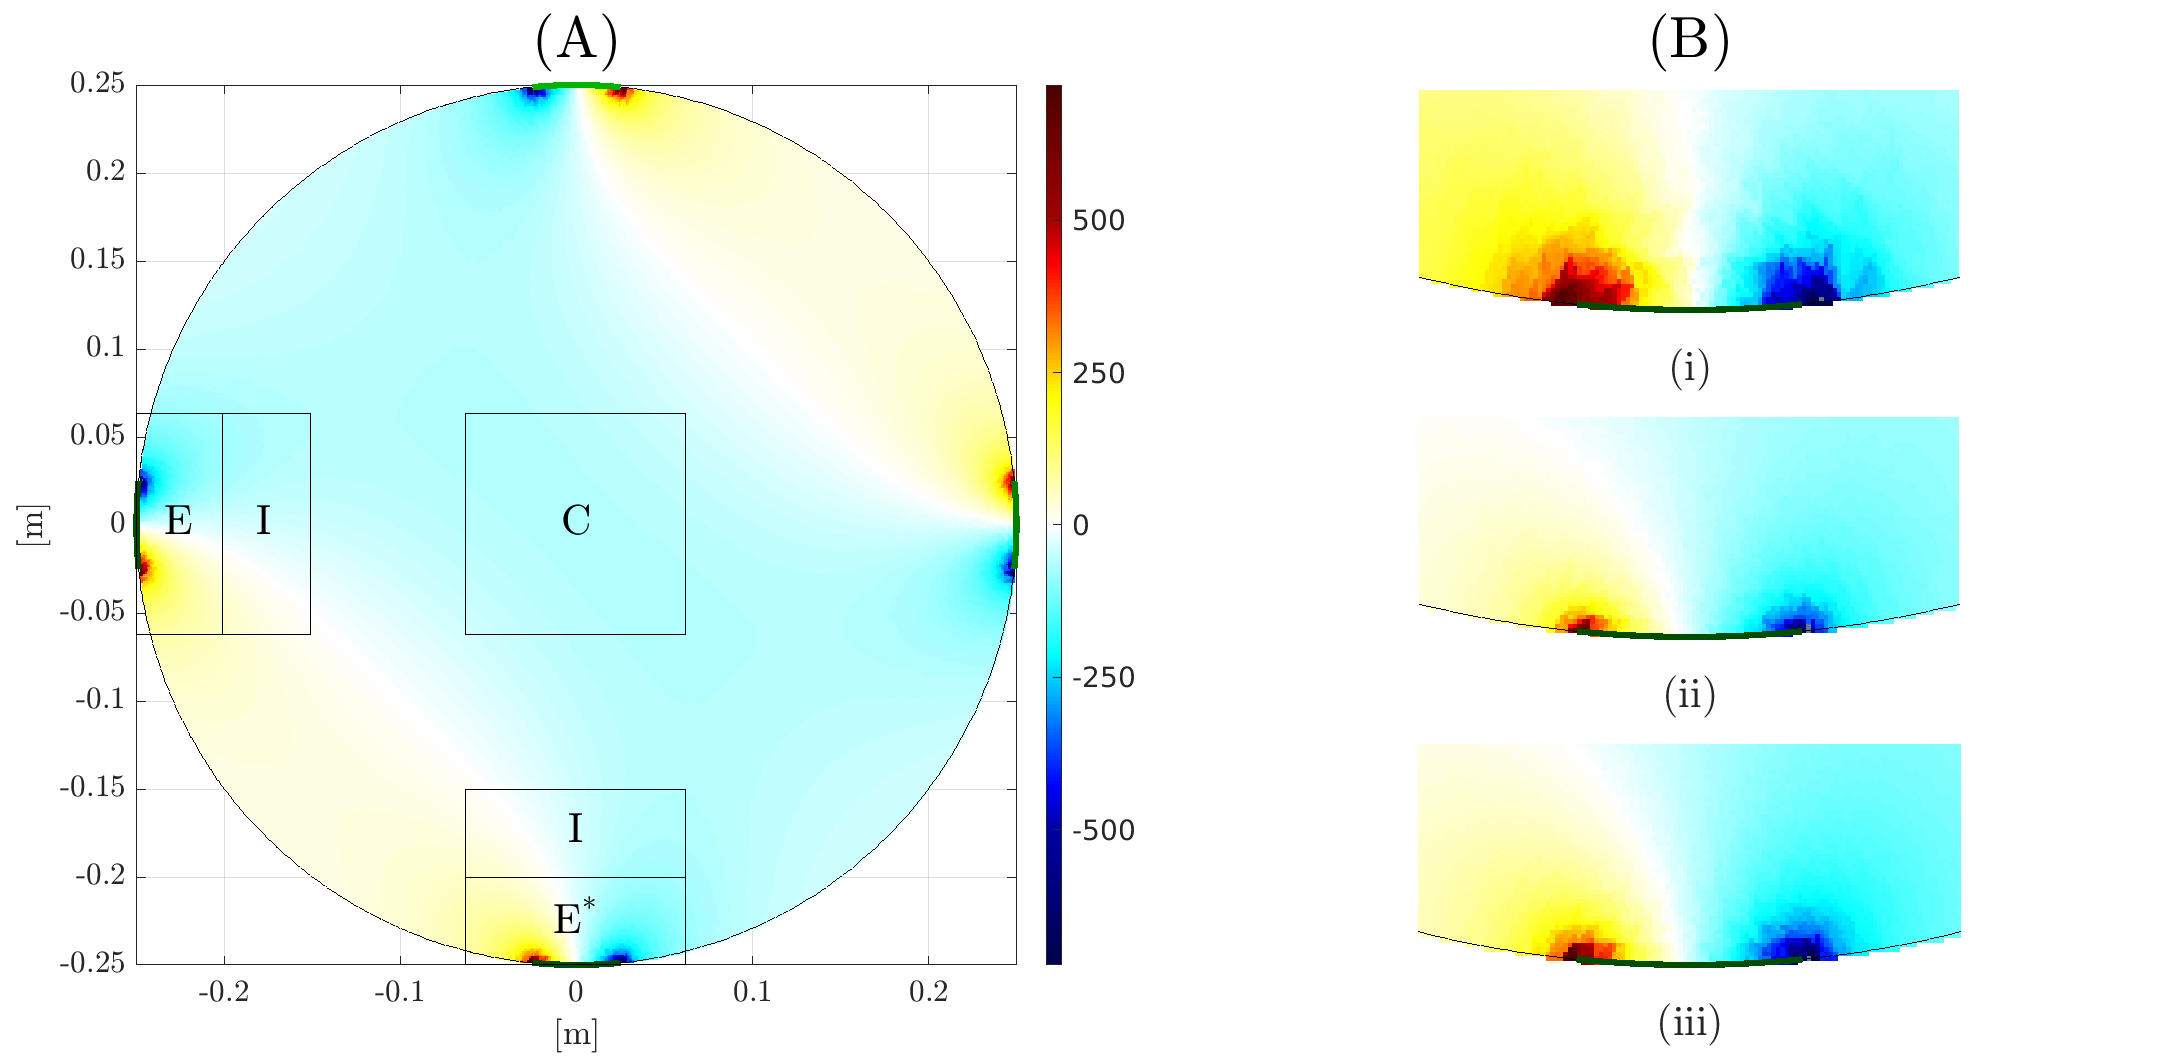
\includegraphics[width=\textwidth,trim={0 0 15cm 1.2cm},clip]{roi_methods_figure.pdf}
	\end{figure}
	\begin{itemize}
		\item Lowest error at approximately 85\% of tank radius
	\end{itemize}
\end{column}
\begin{column}{0.53\textwidth}
	\begin{figure}
		\centering
		\vspace{-5mm}
	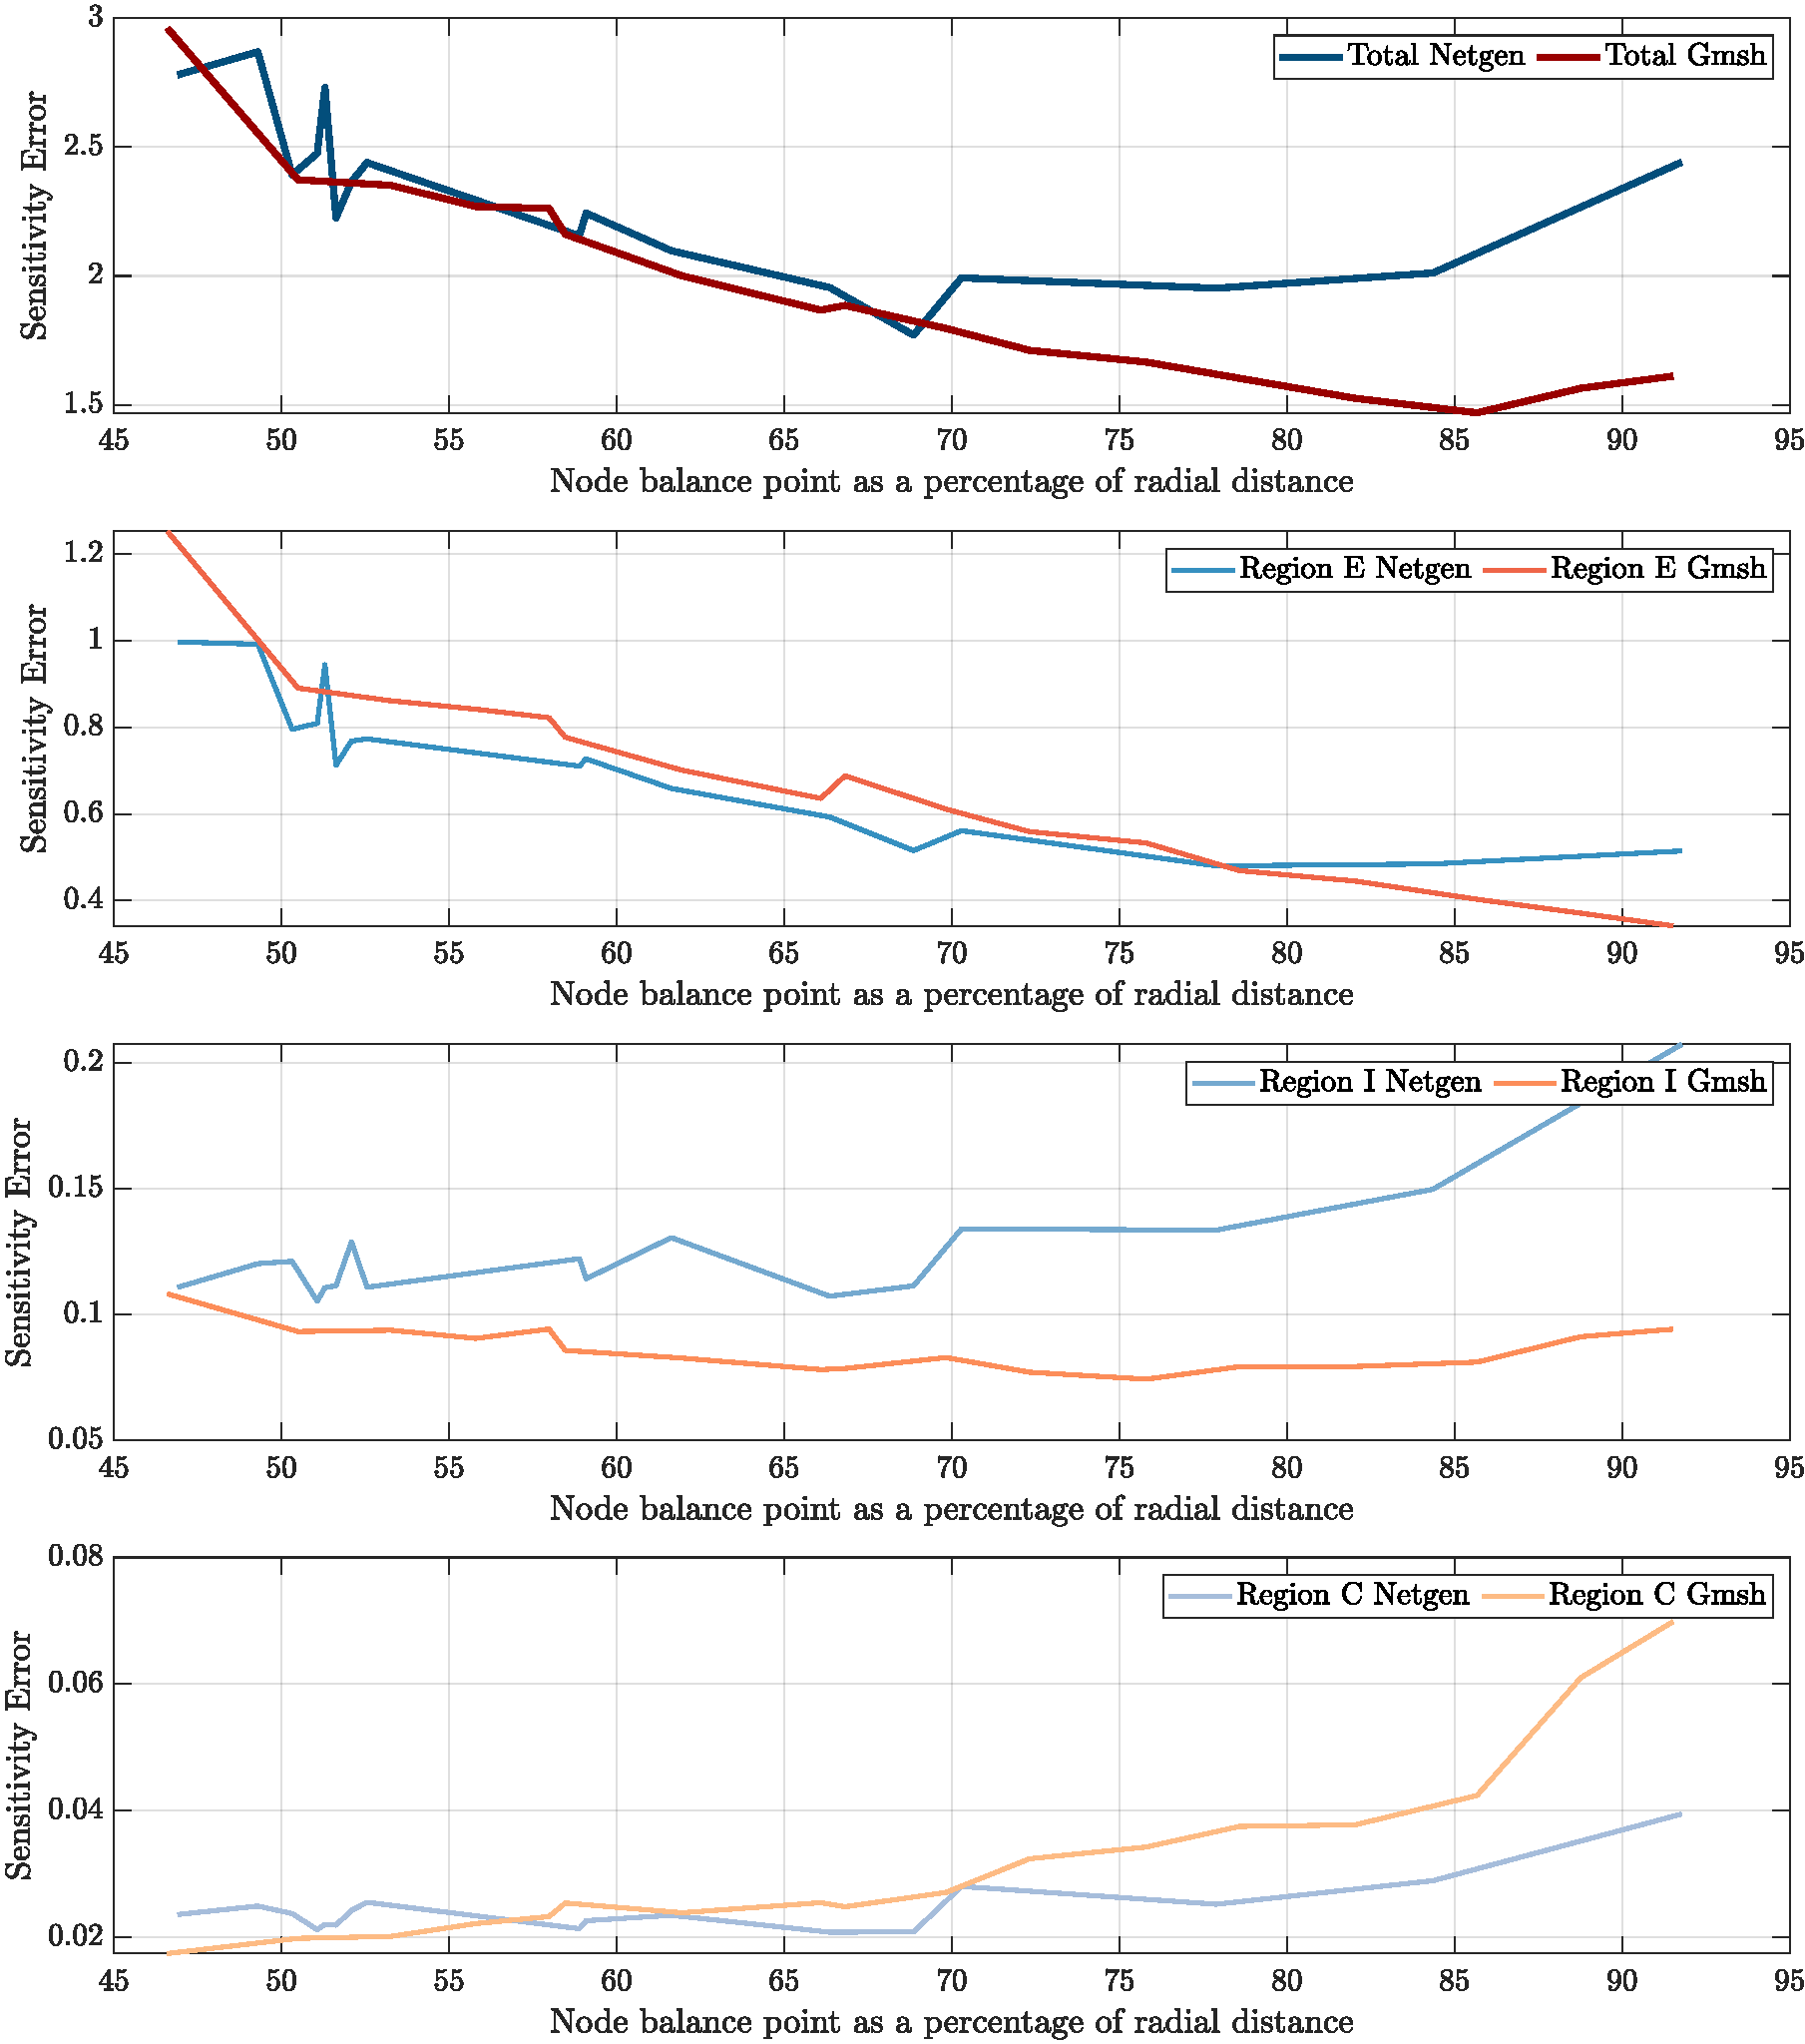
\includegraphics[width=\textwidth,trim={0 0 0cm 0cm},clip]{m-mesh_sens_error_regions_split.pdf}
	\end{figure}
\end{column}
\end{columns}

\end{frame}

\begin{frame}
	\frametitle{Chapter 5: Custom EIT Meshes}
	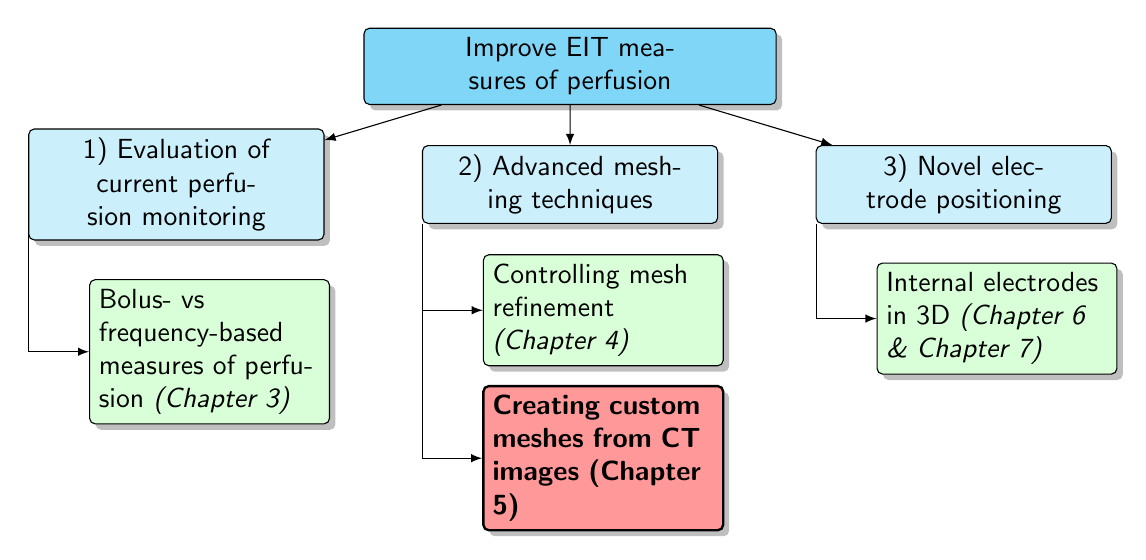
\begin{tikzpicture}[
		level 1/.style={sibling distance=50mm},
		edge from parent/.style={->,draw},
		>=latex]
	  
	  % root of the the initial tree, level 1
	  \node[root] {Improve EIT measures of perfusion}
	  % The first level, as children of the initial tree
		child {node[level 2] (c1) {1) Evaluation of current perfusion monitoring}}
		child {node[level 2] (c2) {2) Advanced meshing techniques}}
		child {node[level 2] (c3) {3) Novel electrode positioning}};
	  
	  % The second level, relatively positioned nodes
	  \begin{scope}[every node/.style={level 3}]
	  \node [below of = c1, xshift=12pt, yshift=-32pt] (c11) {Bolus- vs 
	  frequency-based measures of perfusion \emph{(Chapter 3)}}; 
	  
	  \node [below of = c2, xshift=12pt, yshift=-17pt] (c21) 
	  {Controlling mesh refinement\\ \emph{(Chapter 4)}};
	  \node [below of = c21, yshift=-25pt, fill=red!40 ,line width=0.3mm] (c22) 
	  {\textbf{Creating custom meshes from CT images \emph{(Chapter 5)}}};
	  \node [below of = c3, xshift=12pt, yshift=-20pt] (c31) 
	  {Internal electrodes in 3D \emph{(Chapter 6 \& Chapter 7)}};
	  \end{scope}
	  
	  % lines from each level 1 node to every one of its "children"
	  \foreach \value in {1}
		\draw[->] (c1.195) |- (c1\value.west);
	  
	  \foreach \value in {1,2}
		\draw[->] (c2.195) |- (c2\value.west);
	  
	  \foreach \value in {1}
		\draw[->] (c3.195) |- (c3\value.west);
	  
	  \end{tikzpicture}
\end{frame}




%\begin{frame}
%\frametitle{Chapter 5: Custom EIT Meshes}
%\framesubtitle{ARDS - Acute Respiratory Distress Syndrome}    
%\begin{itemize}
%	\item Widespread inflammation in the lungs 
%	\item Reduces the lungs’ ability to exchange oxygen and carbon dioxide
%	\item Can be diagnosed with chest x-ray 
%	\item Treated with mechanical ventilation
%\end{itemize}
%\end{frame}


%\begin{frame}
%	\frametitle{Chapter 5: Custom EIT Meshes}
%	\framesubtitle{Finitie Element Models (FEMs) in EIT}    
%	\begin{columns}[c]
%		\begin{column}{0.5\textwidth}
%			\begin{figure}[H]
%				\centering
%				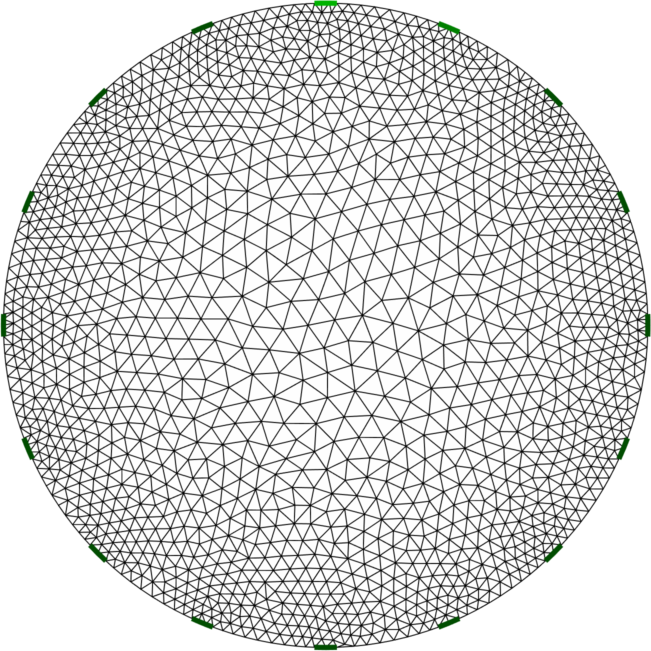
\includegraphics[width=0.9\textwidth]{basic_mesh.png}
%			\end{figure}
%		\end{column}
%		\begin{column}{0.5\textwidth}
%			\begin{itemize}
%				\item \alert{finite element model is required to reconstruct voltages into images}
%				\item The more accurate the FEM the better the reconstruction  
%				\item More prior information regarding the body conductivity is better
%			\end{itemize}
%		\end{column}
%	\end{columns}
%\end{frame}
%
%\begin{frame}
%	\frametitle{Chapter 5: Custom EIT Meshes}
%	\framesubtitle{Finitie Element Models (FEMs) in EIT}    
%	\begin{columns}[c]
%		\begin{column}{0.5\textwidth}
%			\begin{figure}[H]
%				\centering
%				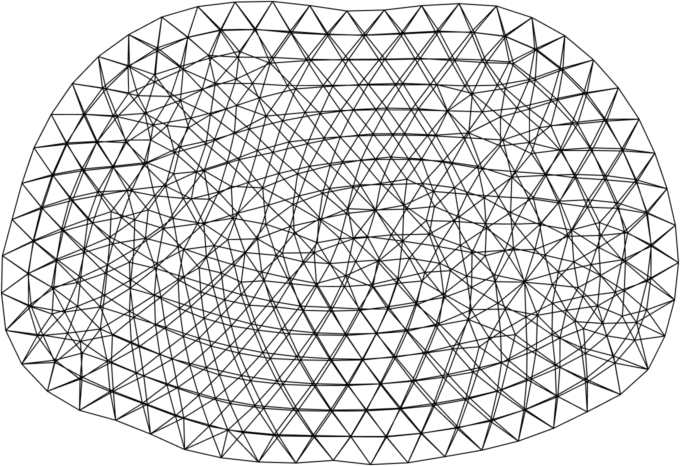
\includegraphics[width=0.9\textwidth]{human_mesh_empty.png}
%			\end{figure}
%		\end{column}
%		\begin{column}{0.5\textwidth}
%			\begin{itemize}
%				\item finite element model is required to reconstruct voltages into images
%				\item \alert{The more accurate the FEM the better the reconstruction} 
%				\item More prior information regarding the body conductivity is better
%			\end{itemize}
%		\end{column}
%	\end{columns}
%\end{frame}

\begin{frame}
	\frametitle{Chapter 5: Custom EIT Meshes}
	\framesubtitle{Introduction}    
	\begin{columns}[c]
		\begin{column}{0.5\textwidth}
			\begin{figure}[H]
				\centering
				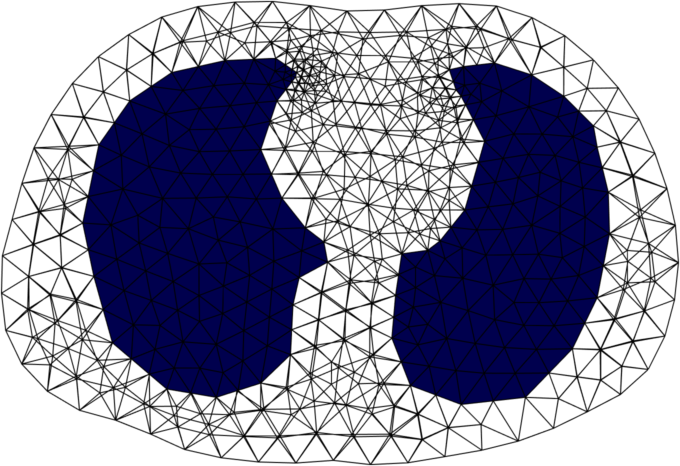
\includegraphics[width=0.9\textwidth]{human_mesh_lungs.png}
			\end{figure}
		\end{column}
		\begin{column}{0.5\textwidth}
			\begin{itemize}
				\item A finite element model is required to reconstruct voltages into images
				\item The more accurate the FEM, the better the reconstruction
				\item More prior information regarding the body conductivity
				\item For some patients (ARDS) we have diagnostic CT images 
			\end{itemize}
		\end{column}
	\end{columns}%
	\vspace{8mm}
\alert{Can we use this to improve EIT image reconstruction and monitoring of patients?}
\end{frame}

%\begin{frame}
%	\frametitle{Motivation}    
%	\begin{itemize}
%		\item Often a generic model is used for reconstructions
%		\item True electrode locations and internal geometry is unknown  
%		\item With ARDS patients we have information from  diagnostic CT images
%		\item More prior information 
%	\end{itemize}
%\vspace{2em}
%\alert{Can we use this to improve EIT image reconstruction and monitoring of patients?}
%\end{frame}

%\begin{frame}
%	\frametitle{Overview}    
%	\begin{enumerate}
%		\item Obtain CT images
%		\item Automatically identify lung regions  
%		\item Present in a GUI for correction by doctors or technicians
%		\item Generate a FEM based on the corrected segmentation
%		\item Reconstruct EIT data
%	\end{enumerate}
%\end{frame}
% 
% \begin{frame}
% 	\frametitle{CT images}    
%		\begin{figure}[H]
%			\centering
%			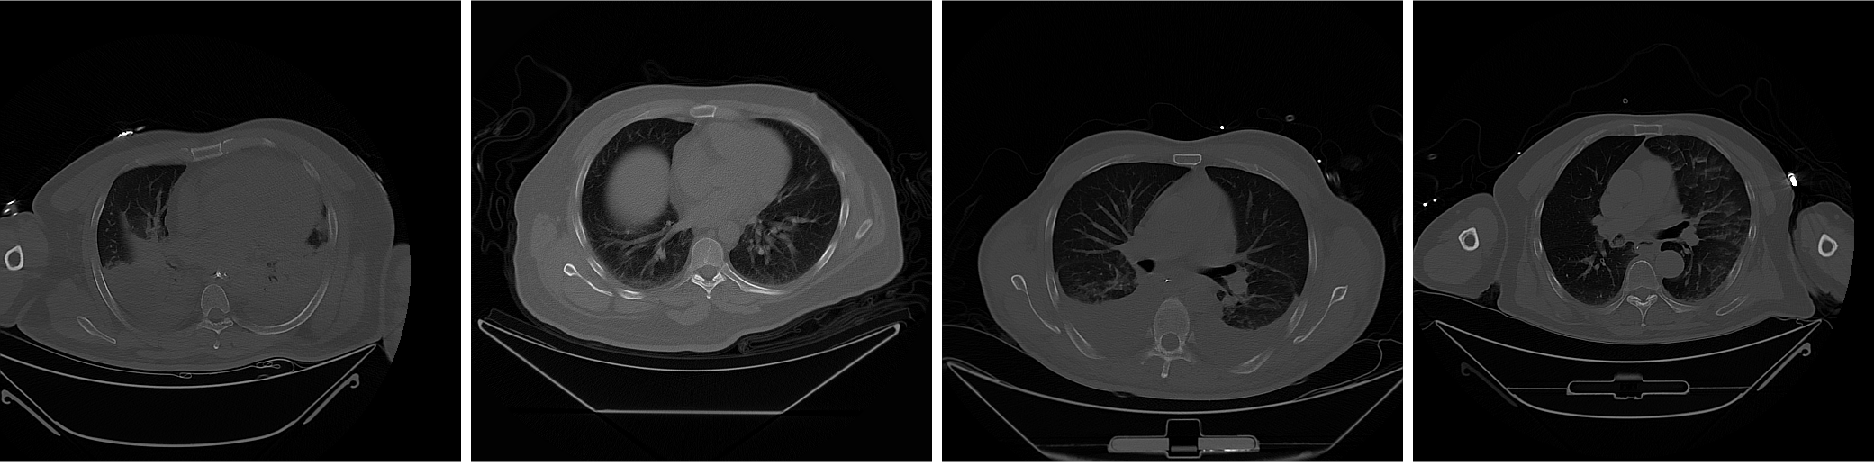
\includegraphics[width=\textwidth]{raw_ct_imgs.png}
%		\end{figure}
%	Example images taken from the 4th intercostal space for each subject
% \end{frame}
 
\begin{frame}
	\frametitle{Chapter 5: Custom EIT Meshes}
	\framesubtitle{Methods: Automatic Segmentation}    
		\begin{figure}[H]
			\centering
			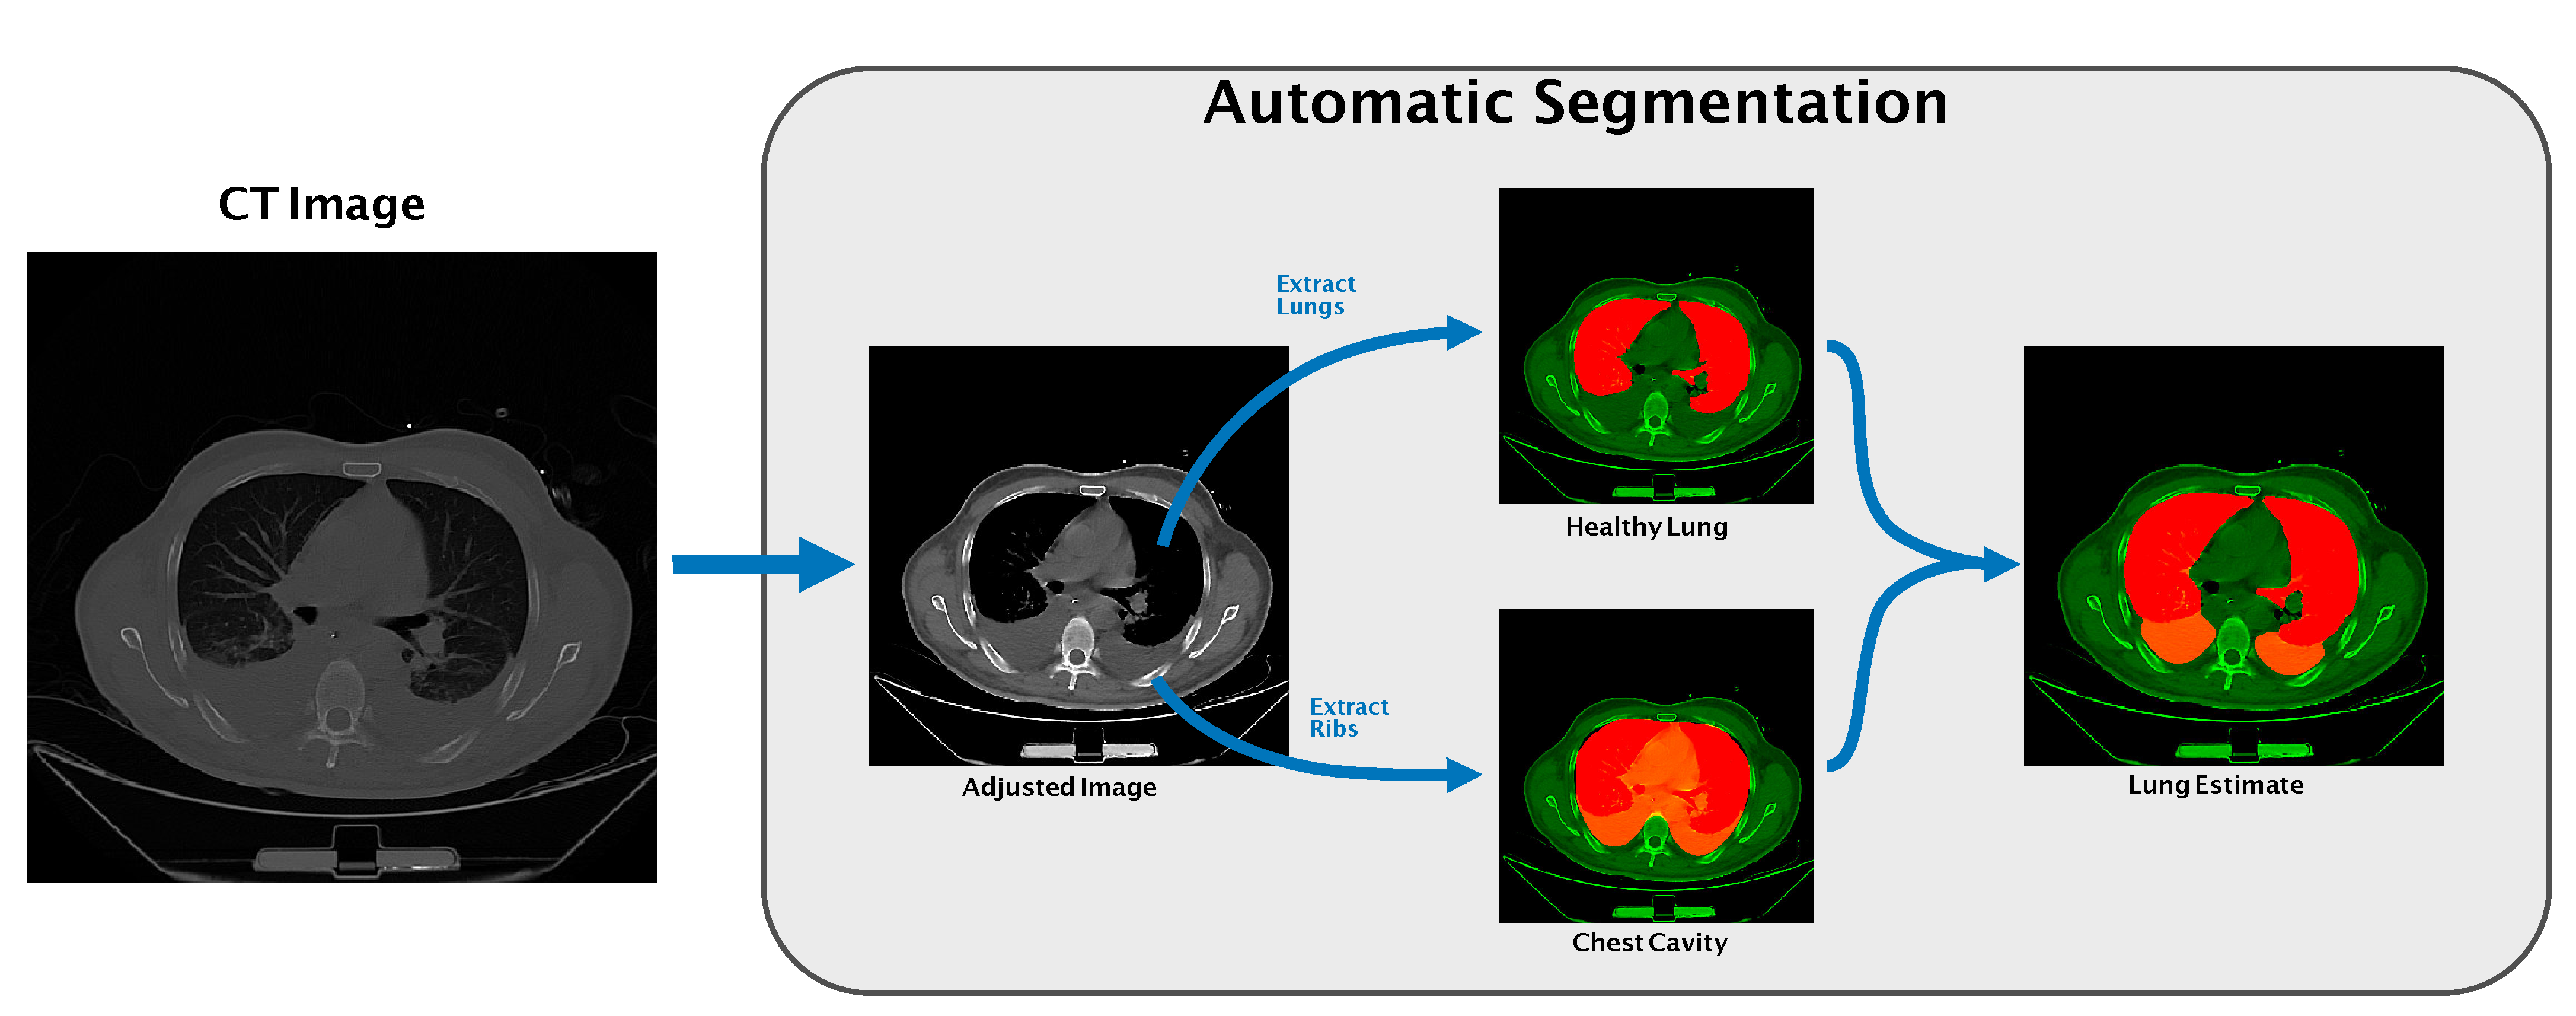
\includegraphics[width=\textwidth]{lung_segmentation_methods_a.pdf}
		\end{figure}
\end{frame}

%\begin{frame}
%	\frametitle{Segmentation Results}    
%	\begin{figure}[H]
%		\centering
%		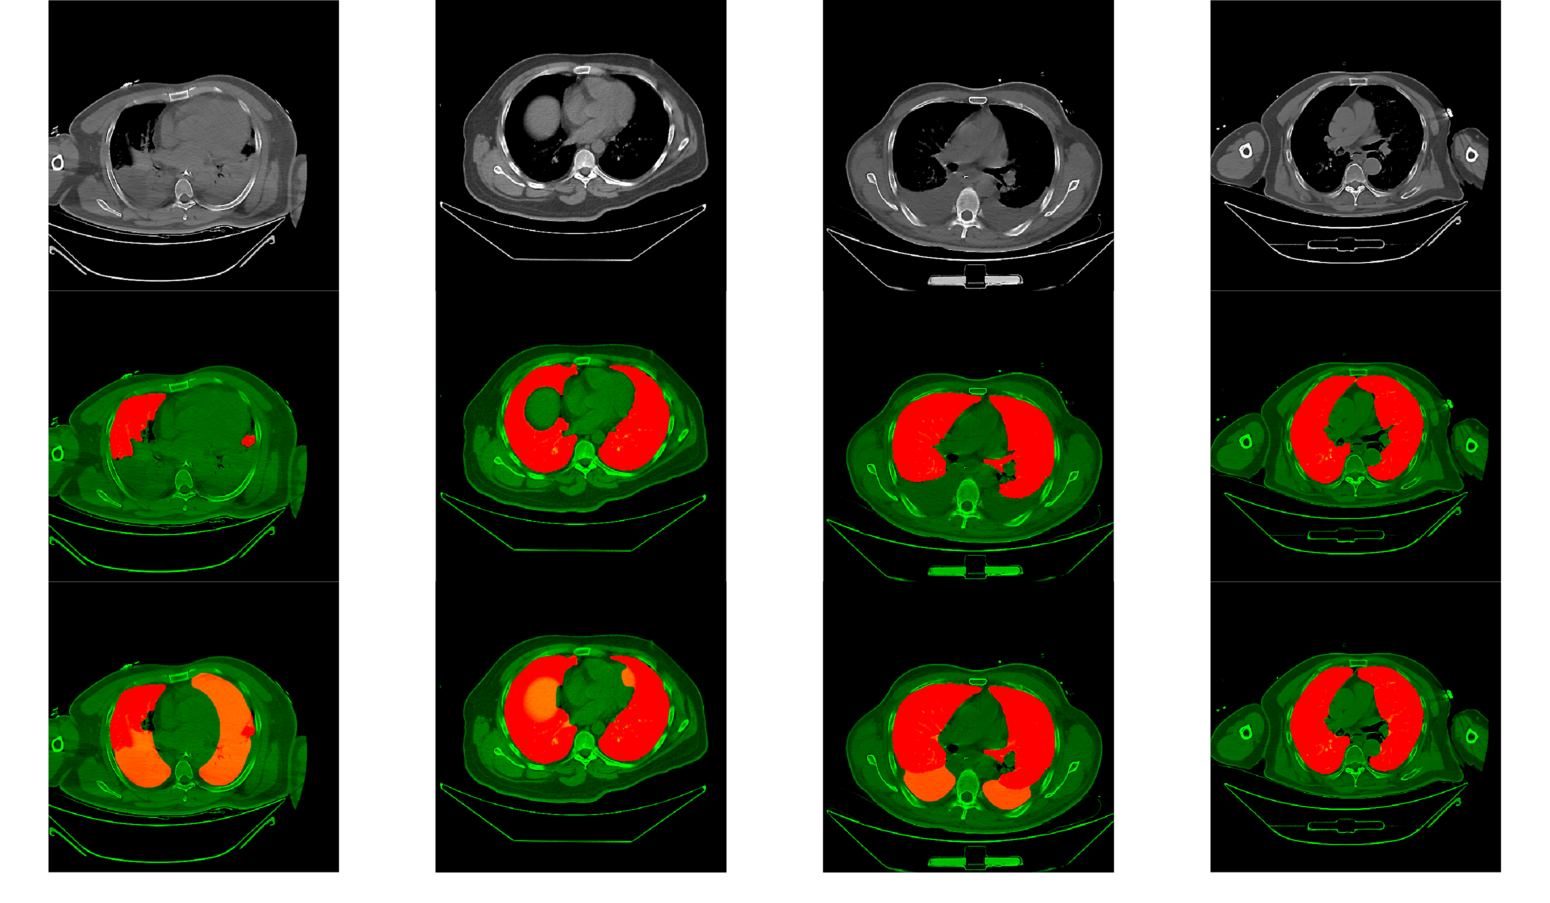
\includegraphics[width=\textwidth]{segment_results.png}
%	\end{figure}
%\end{frame}

\begin{frame}
	\frametitle{Chapter 5: Custom EIT Meshes}
	\framesubtitle{Methods: Manual Correction}    
	\begin{figure}[H]
		\centering
		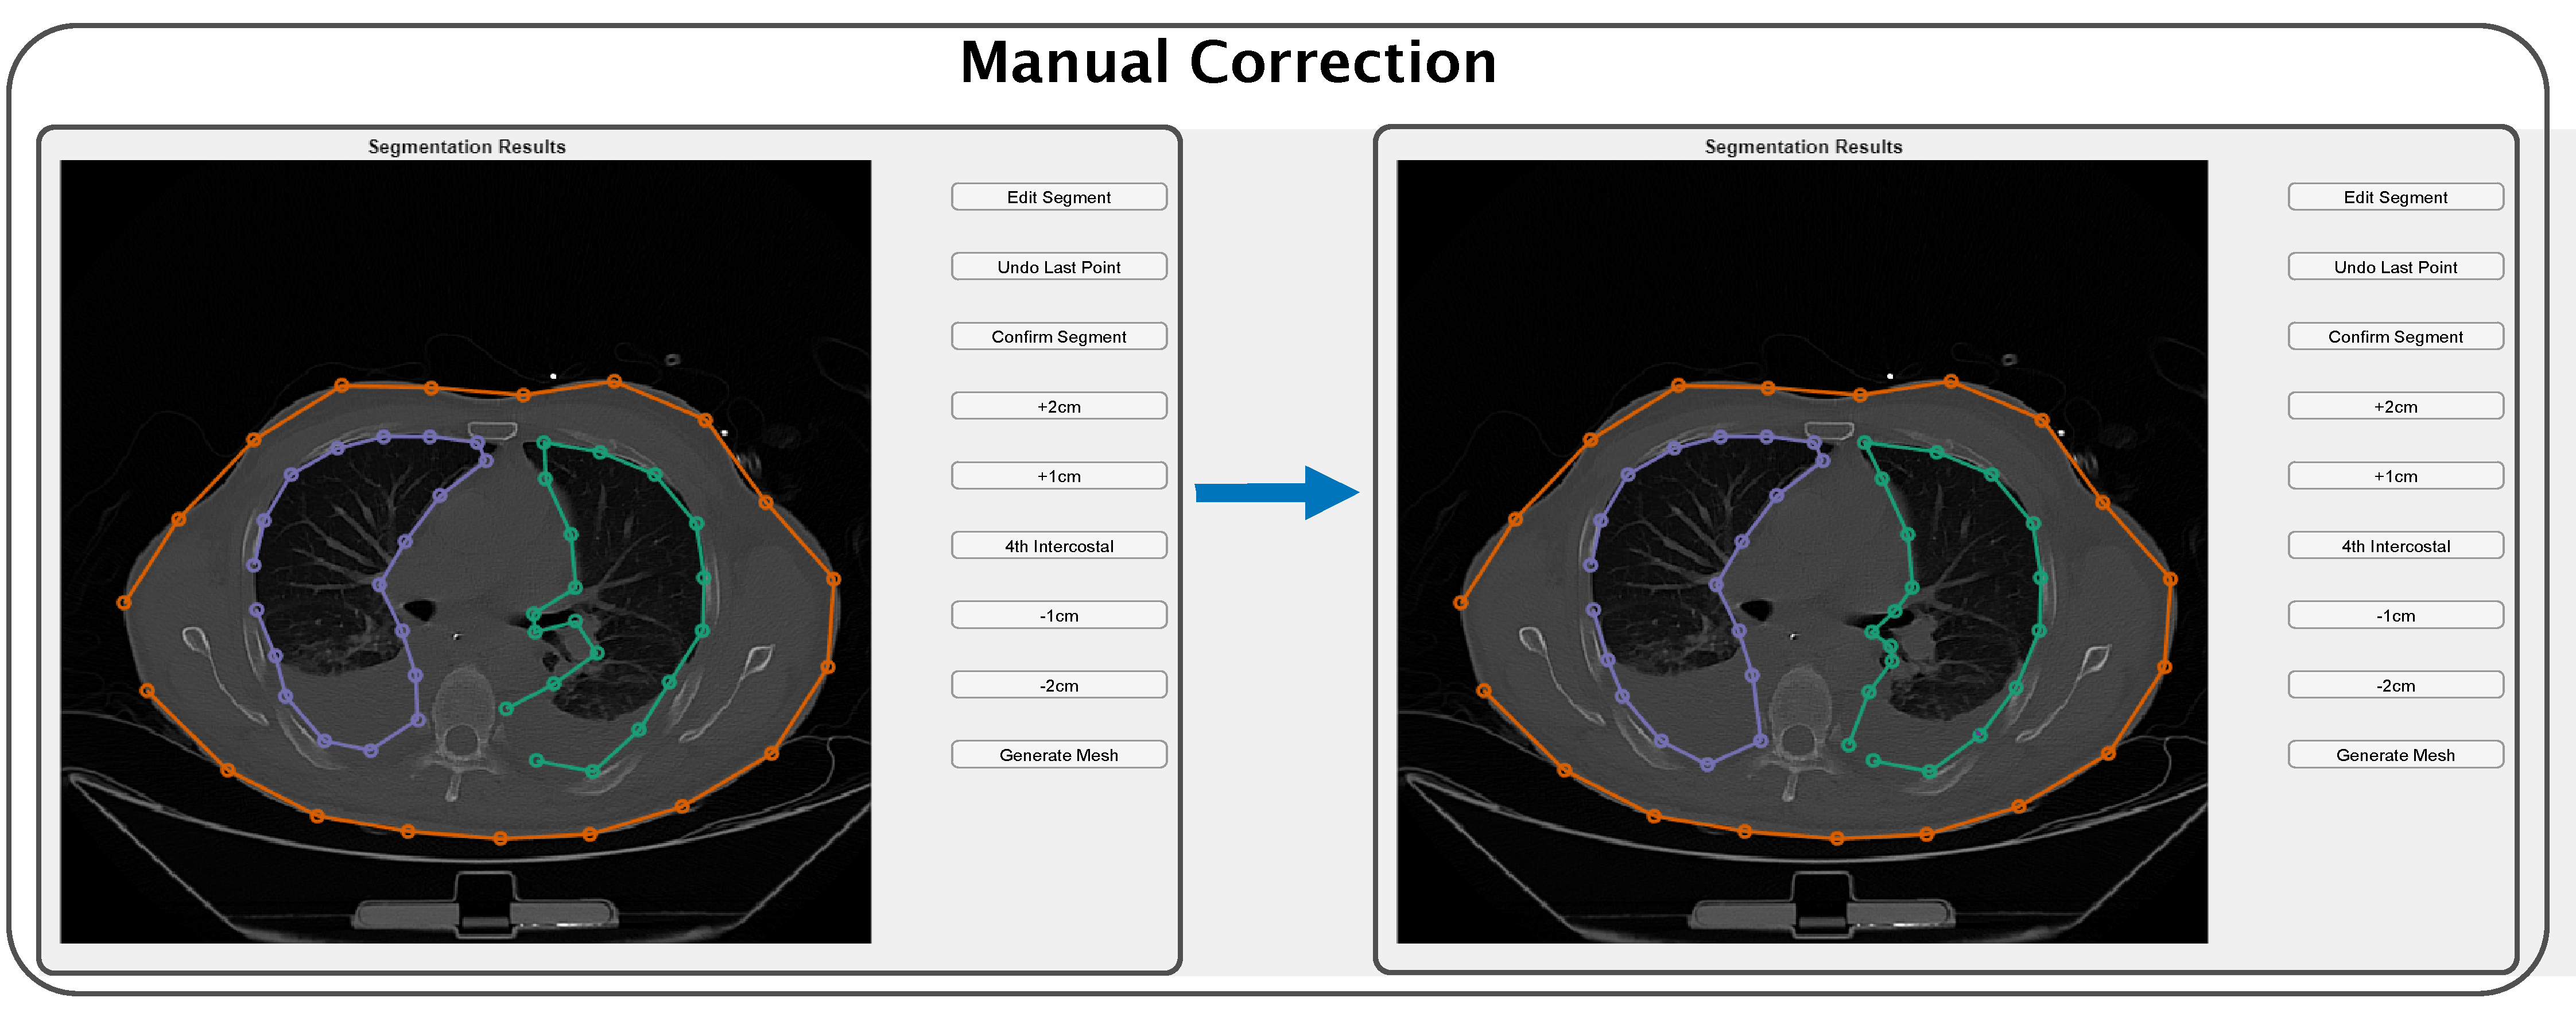
\includegraphics[width=\textwidth]{lung_segmentation_methods_b.pdf}
	\end{figure}
\end{frame}

\begin{frame}
	\frametitle{Chapter 5: Custom EIT Meshes}
	\framesubtitle{Methods: Meshing}    
	\begin{figure}[H]
		\centering
		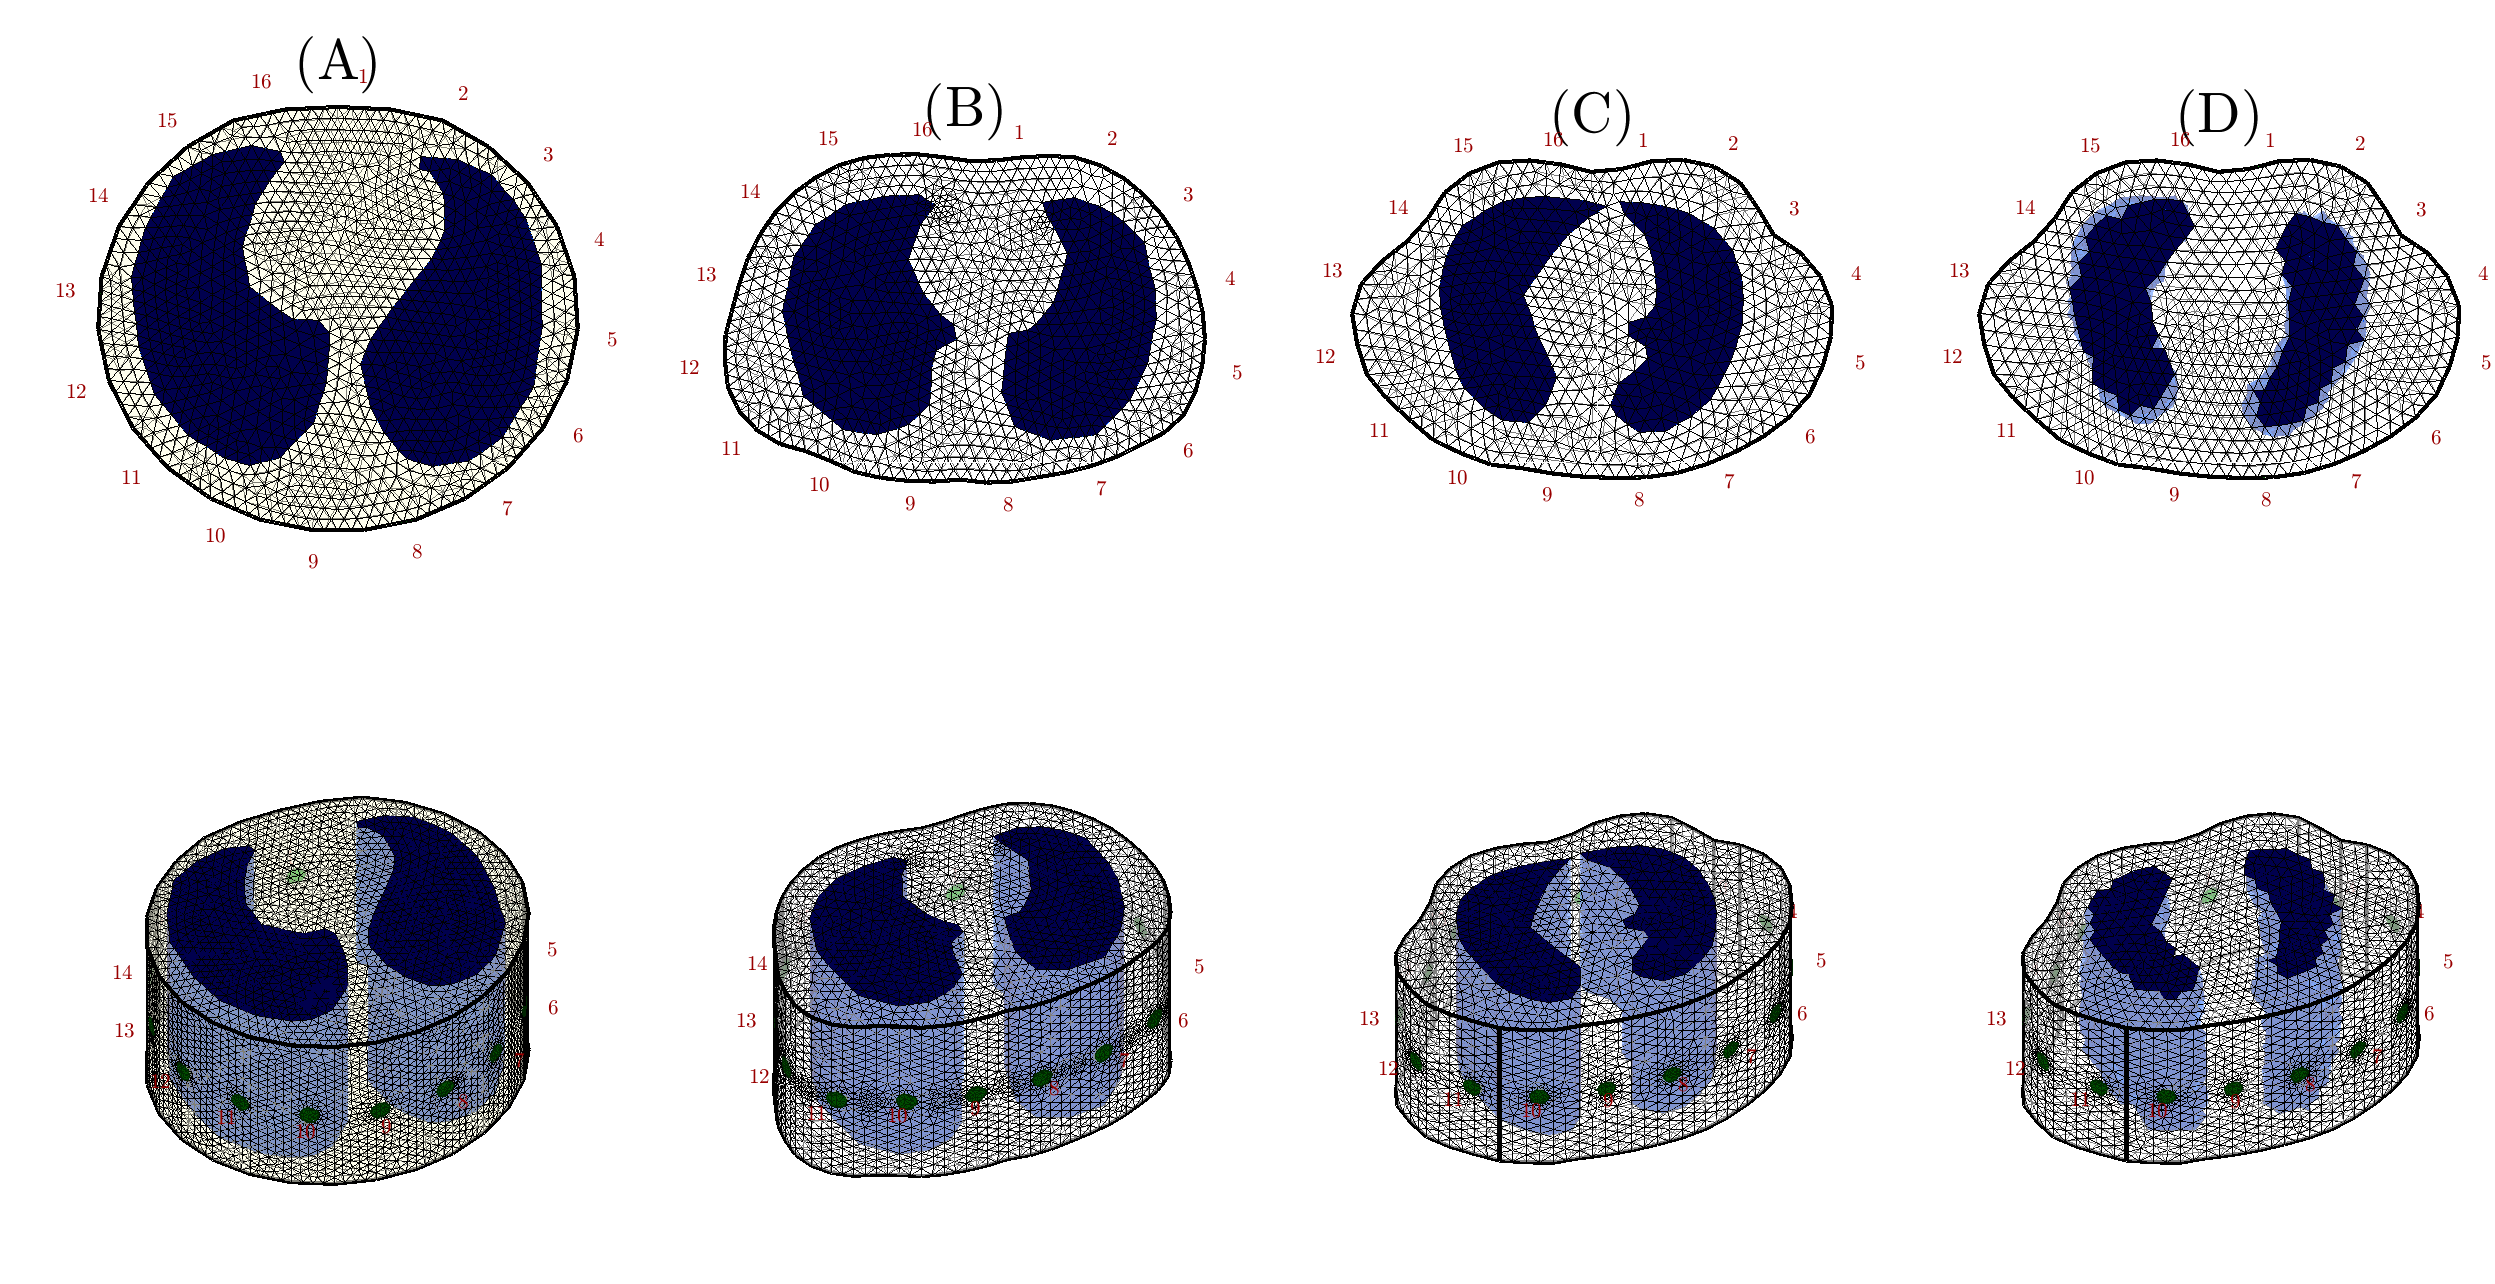
\includegraphics[width=\textwidth]{fem_models_PT04.pdf}
	\end{figure}
\end{frame}

\begin{frame}
	\frametitle{Chapter 5: Custom EIT Meshes}
	\framesubtitle{Results}   
	Center of ventilation error relative to the CT centre of ventilation.
	\\ \vspace{2mm}
	\begin{figure}[H]
		\centering
		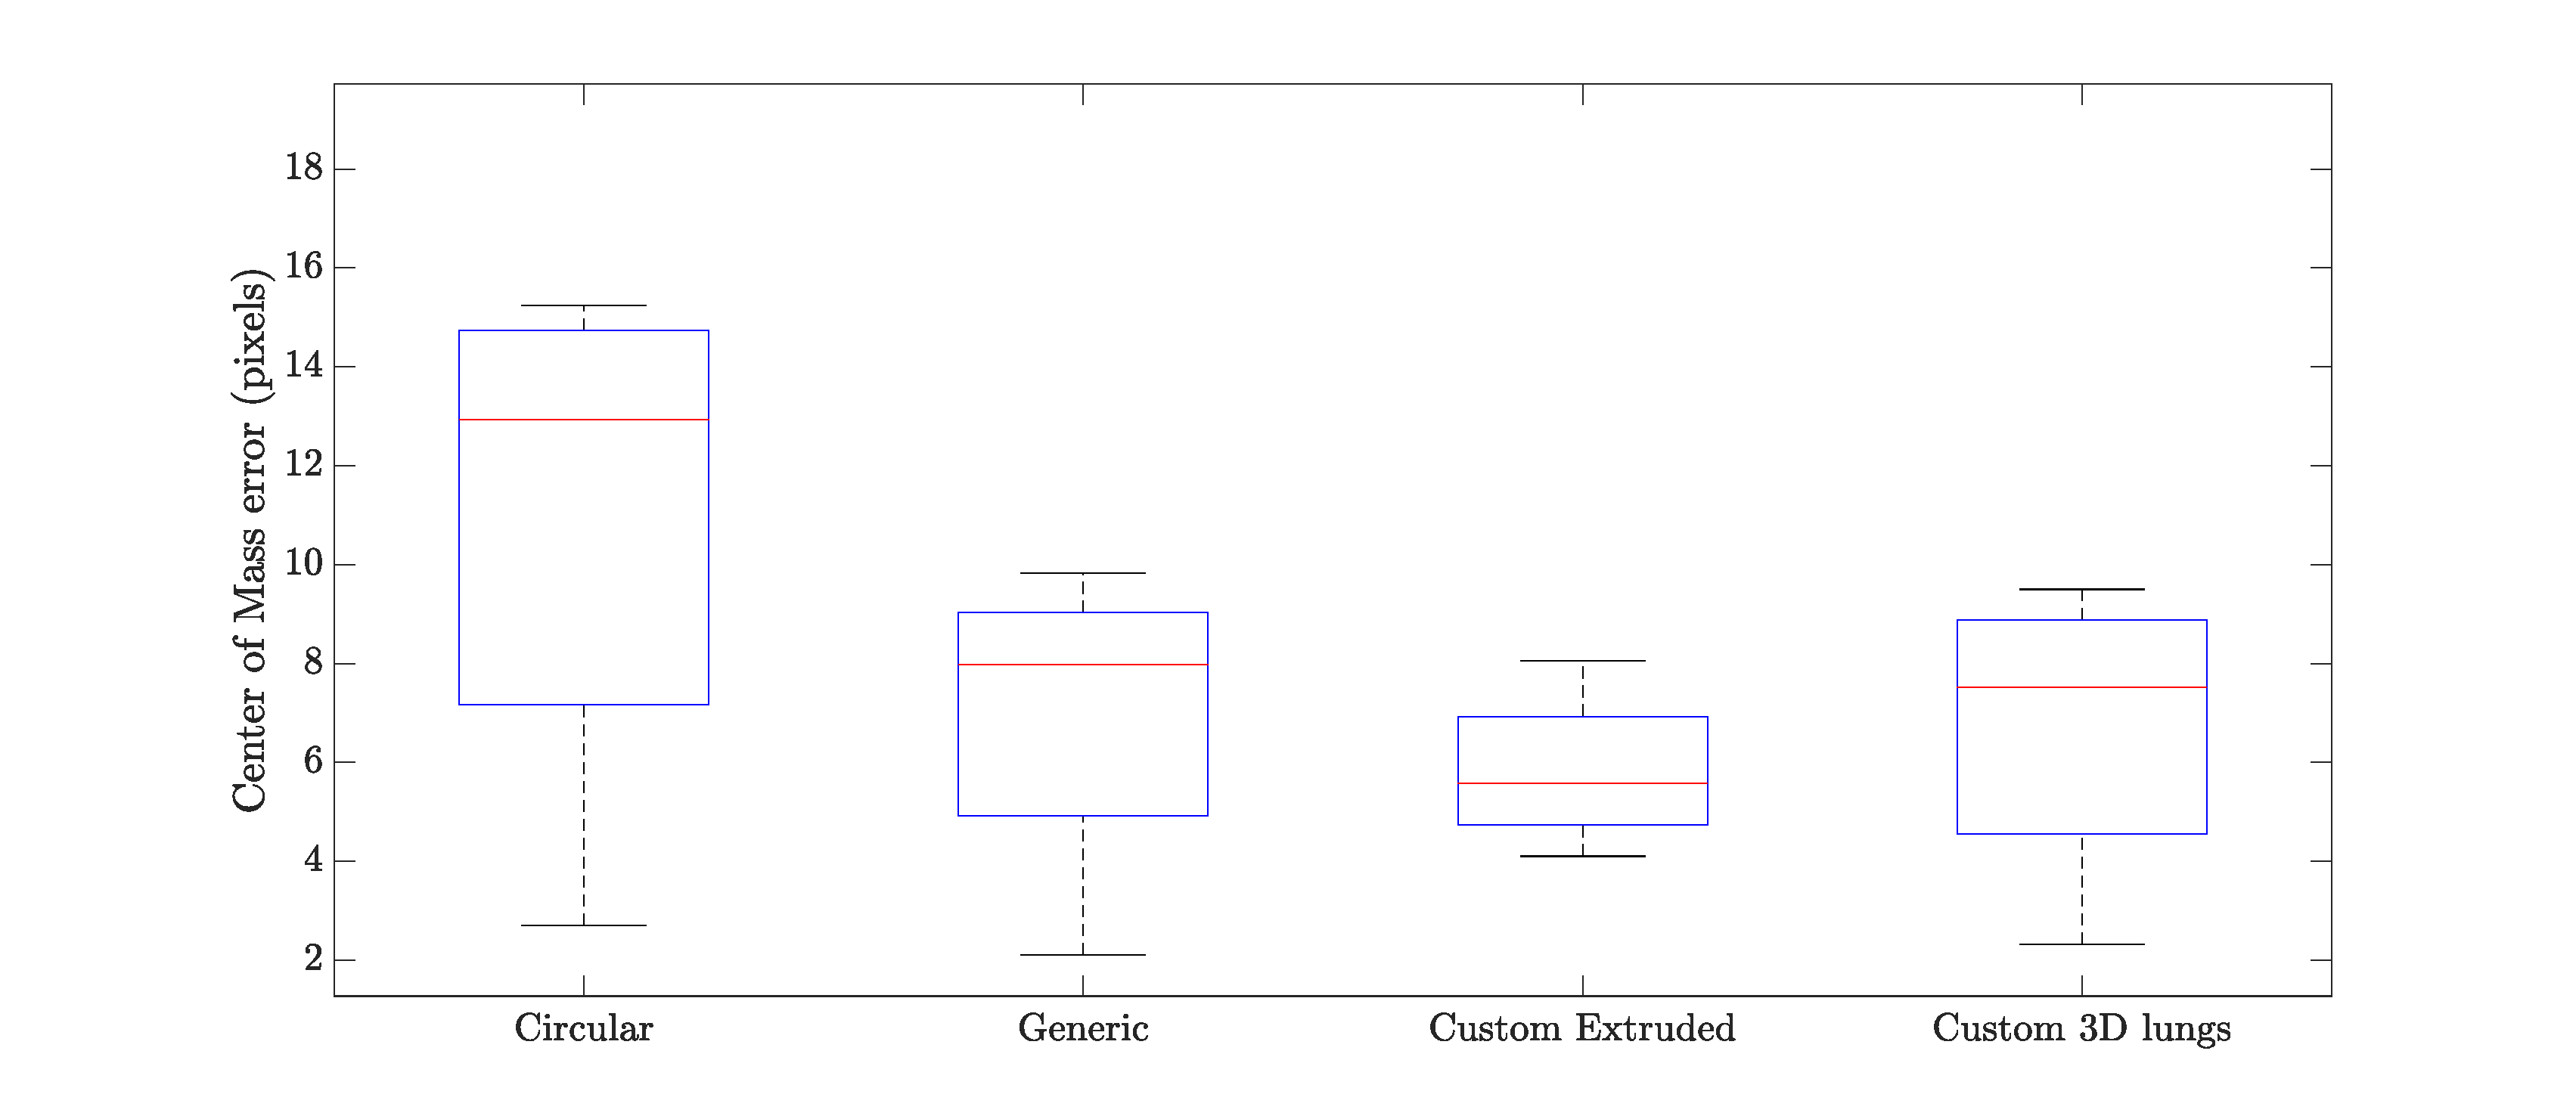
\includegraphics[width=0.9\textwidth,trim={0 1.5cm 0 1.5cm},clip]{error_boxplot.pdf}
	\end{figure}%
	%\\ 
	\vspace{1mm}
	Custom model is lower, but not consistently. 
	\\ \vspace{5mm}
	\centering
	\alert{Electrode locations are still unknown...}
\end{frame}


\begin{frame}
	\frametitle{Chapter 6: Internal Electrode Sensitivity}
	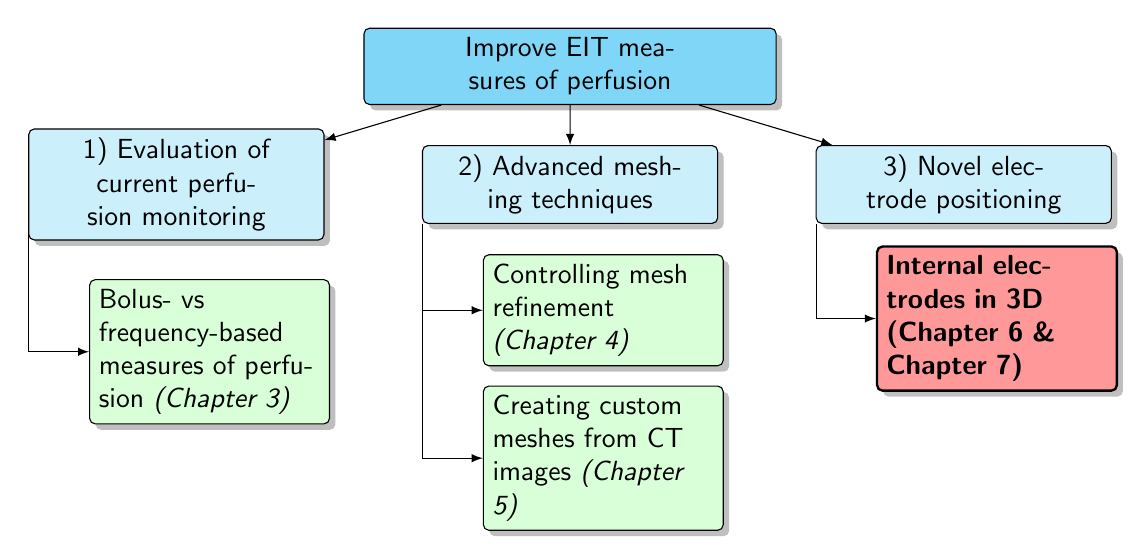
\begin{tikzpicture}[
		level 1/.style={sibling distance=50mm},
		edge from parent/.style={->,draw},
		>=latex]
	  
	  % root of the the initial tree, level 1
	  \node[root] {Improve EIT measures of perfusion}
	  % The first level, as children of the initial tree
		child {node[level 2] (c1) {1) Evaluation of current perfusion monitoring}}
		child {node[level 2] (c2) {2) Advanced meshing techniques}}
		child {node[level 2] (c3) {3) Novel electrode positioning}};
	  
	  % The second level, relatively positioned nodes
	  \begin{scope}[every node/.style={level 3}]
	  \node [below of = c1, xshift=12pt, yshift=-32pt] (c11) {Bolus- vs 
	  frequency-based measures of perfusion \emph{(Chapter 3)}}; 
	  
	  \node [below of = c2, xshift=12pt, yshift=-17pt] (c21) 
	  {Controlling mesh refinement\\ \emph{(Chapter 4)}};
	  \node [below of = c21, yshift=-25pt] (c22) 
	  {Creating custom meshes from CT images \emph{(Chapter 5)}};
	  \node [below of = c3, xshift=12pt, yshift=-20pt, fill=red!40 ,line width=0.3mm] (c31) 
	  {\textbf{Internal electrodes in 3D \emph{(Chapter 6 \& Chapter 7)}}};
	  \end{scope}
	  
	  % lines from each level 1 node to every one of its "children"
	  \foreach \value in {1}
		\draw[->] (c1.195) |- (c1\value.west);
	  
	  \foreach \value in {1,2}
		\draw[->] (c2.195) |- (c2\value.west);
	  
	  \foreach \value in {1}
		\draw[->] (c3.195) |- (c3\value.west);
	  
	  \end{tikzpicture}
\end{frame}

\begin{frame}
	\frametitle{Chapter 6: Internal Electrode Sensitivity}
	\framesubtitle{Introduction}
	To increase sensitivity in the centre of a model internal electrodes are added.  \\ \vspace{3mm}
	\begin{figure}[H]
		\centering
		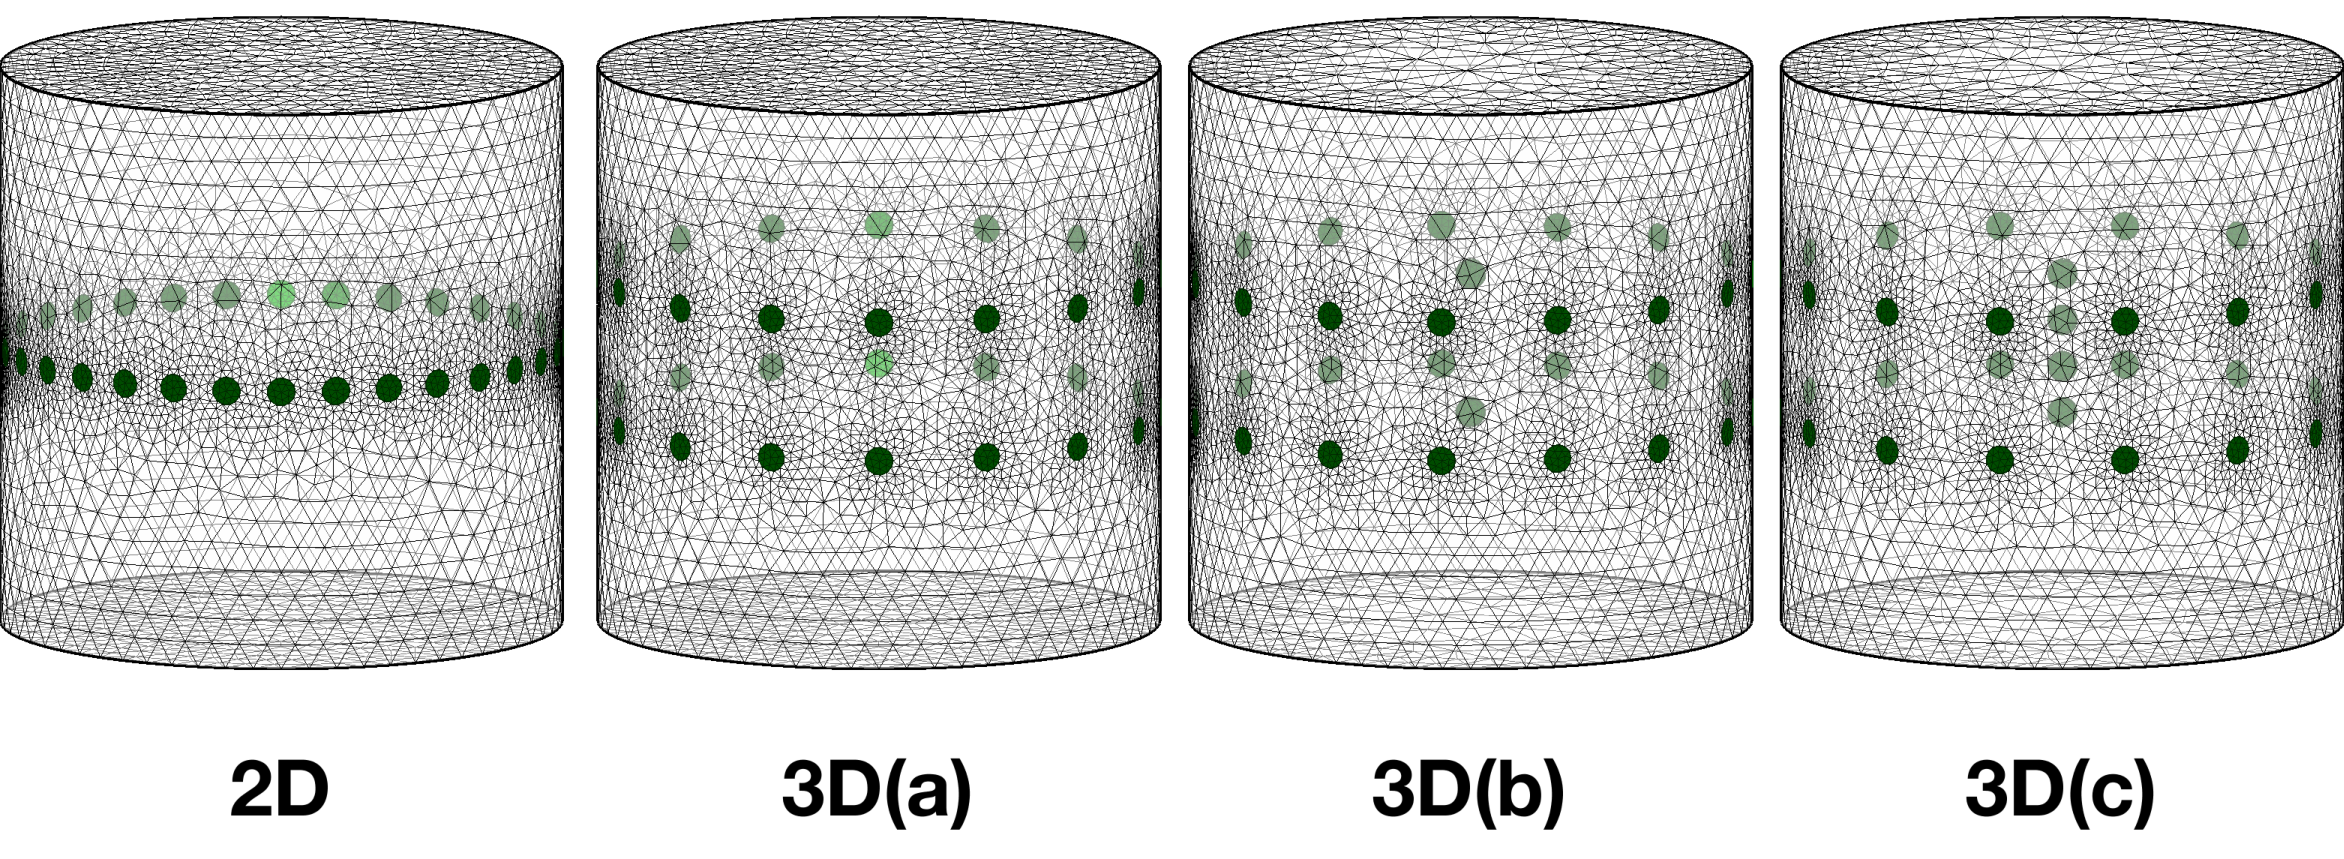
\includegraphics[width=0.9\textwidth,trim={0 0.5cm 0 0cm},clip]{FEM_Comparison.pdf}
	\end{figure}%
	Typical 2D and 3D configurations are compared to internal electrode configurations.
\end{frame}

\begin{frame}
	\frametitle{Chapter 6: Internal Electrode Sensitivity}
	\framesubtitle{Results}
	\begin{figure}[H]
		\centering
		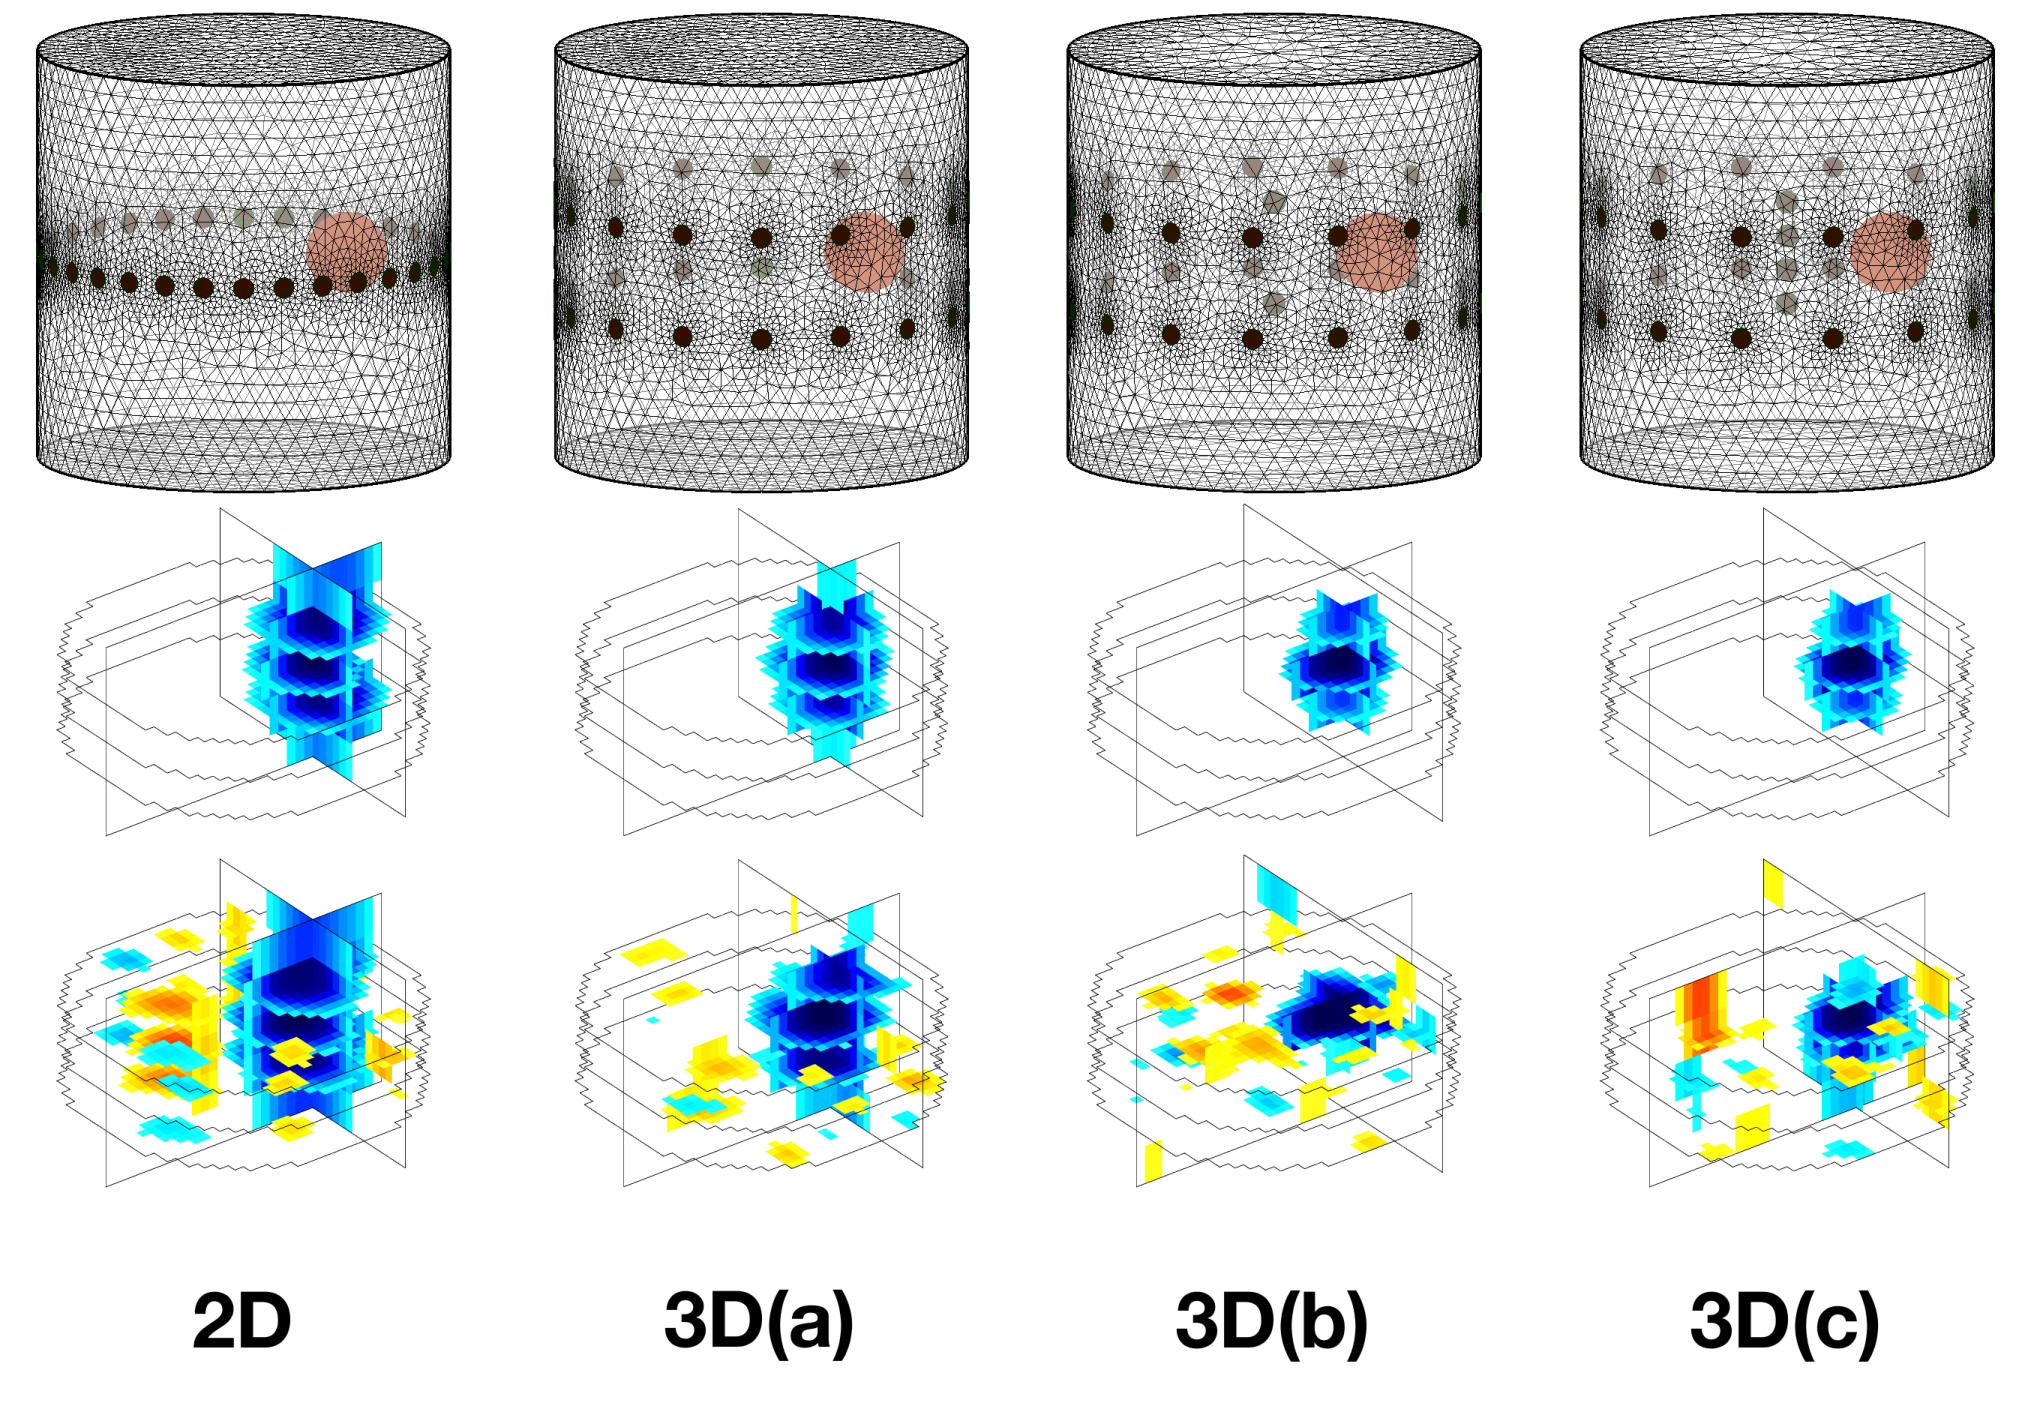
\includegraphics[width=0.65\textwidth,trim={0 0.5cm 0 0cm},clip]{Image_Comparison.pdf}
	\end{figure}%
	Internal electrodes were used to reconstruct the target closer to actual size.
\end{frame}

\begin{frame}
	\frametitle{Chapter 6: Internal Electrode Sensitivity}
	\framesubtitle{Results}
	\begin{figure}[H]
		\centering
		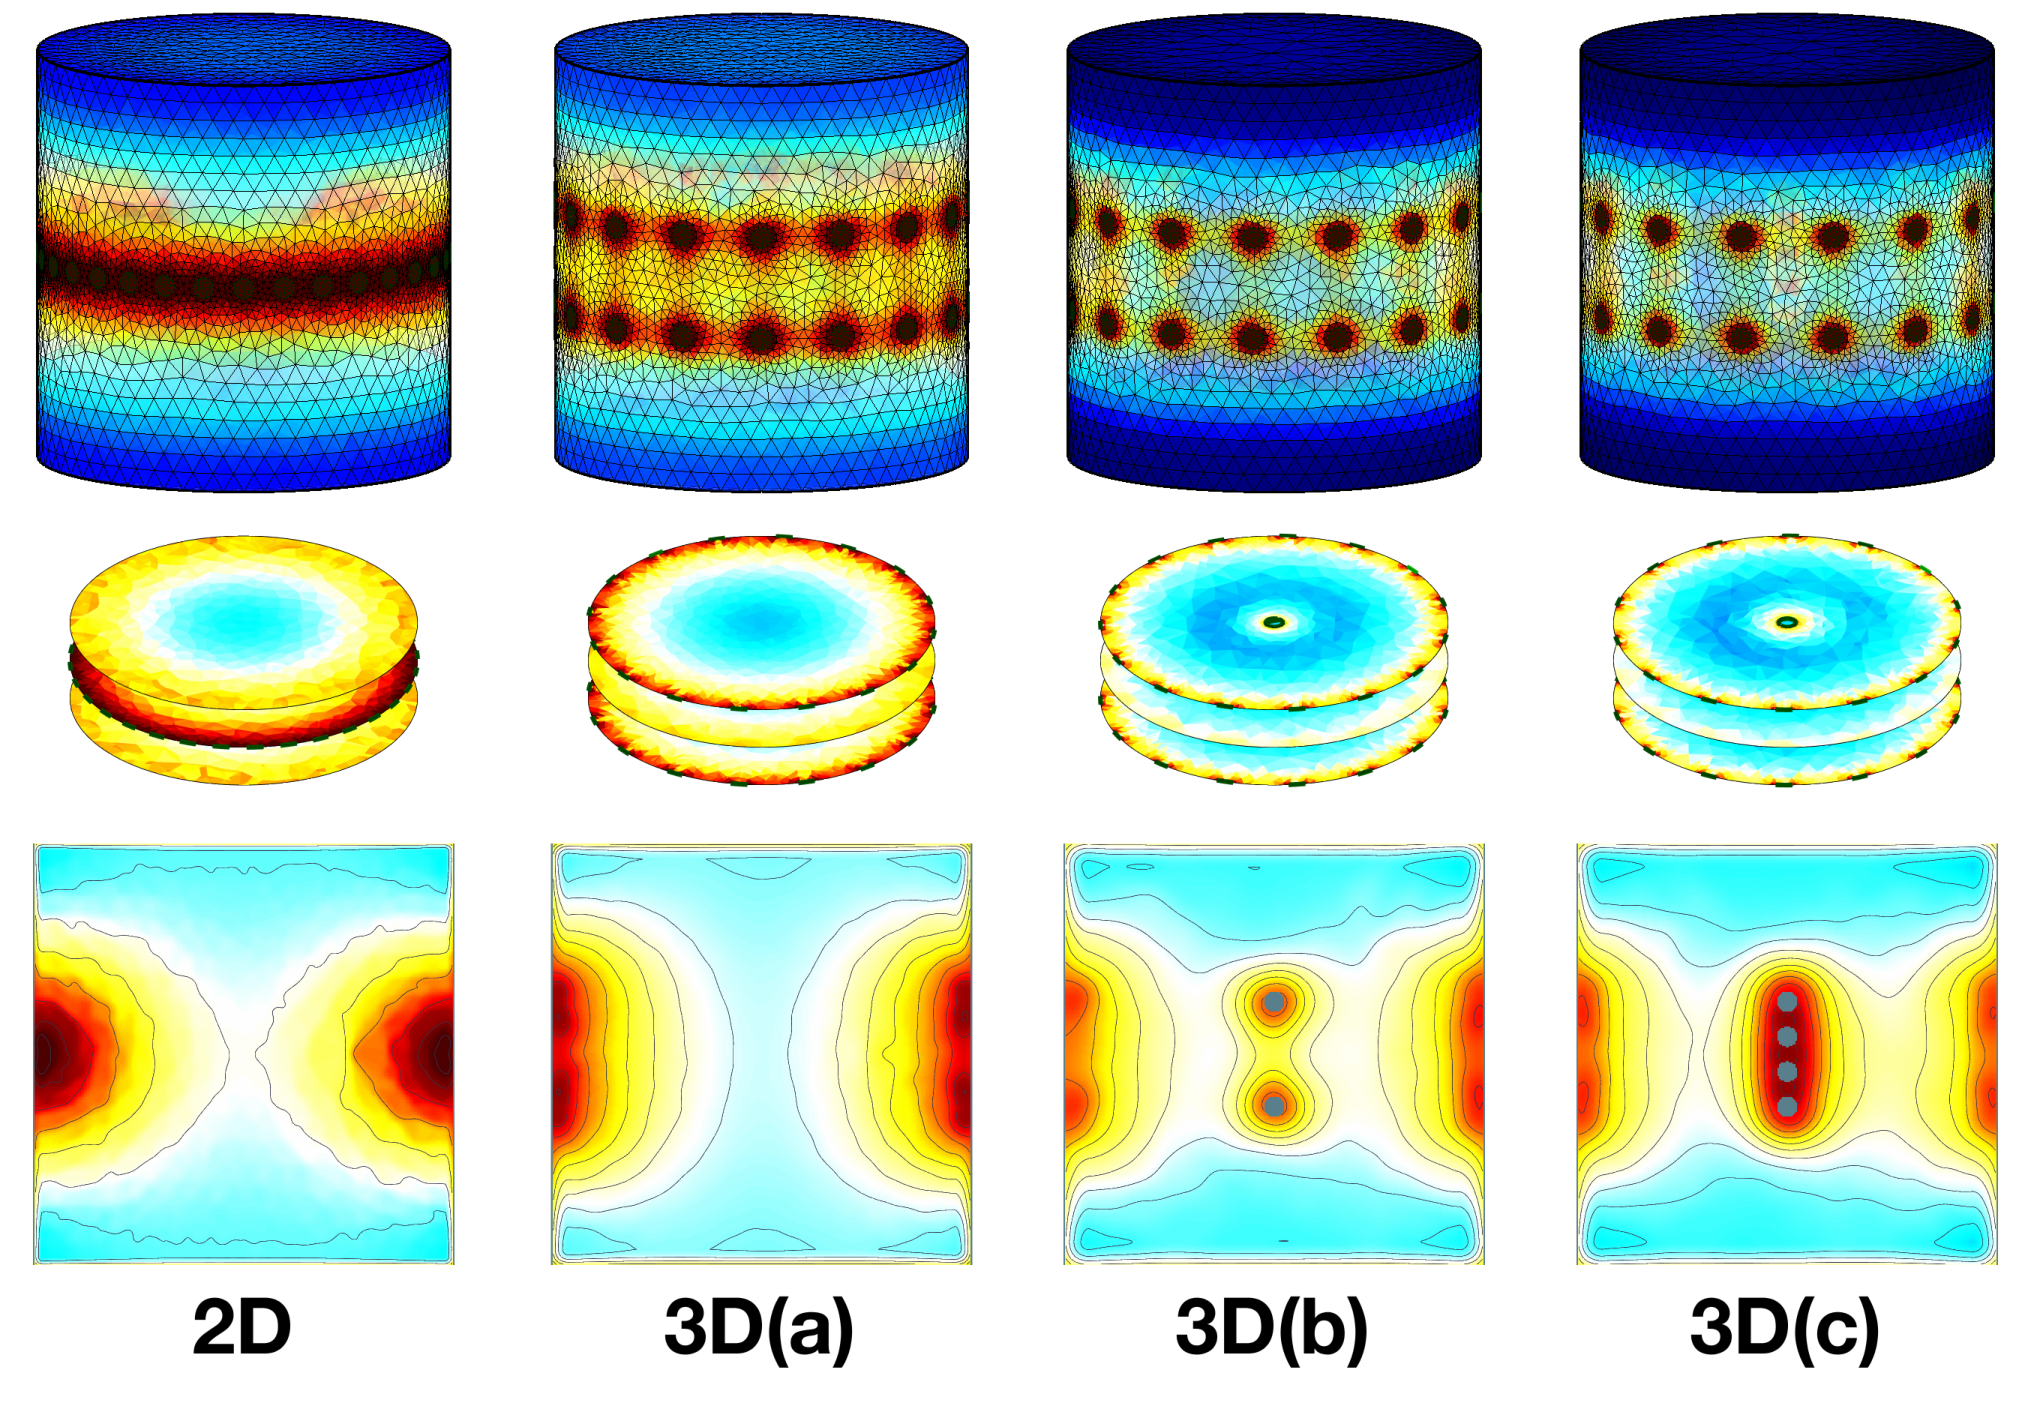
\includegraphics[width=0.65\textwidth,trim={0 0.5cm 0 0cm},clip]{Sensitivity_Comparison_new.pdf}
	\end{figure}%
	With high sensitivity near the internal electrodes, small internal errors can produce large artefacts.
\end{frame}

\begin{frame}
	\frametitle{Chapter 7: Internal Electrode Motion}
	\framesubtitle{Introduction}
	\begin{columns}[c]
		\begin{column}{0.5\textwidth}
			\begin{figure}[H]
				\centering
				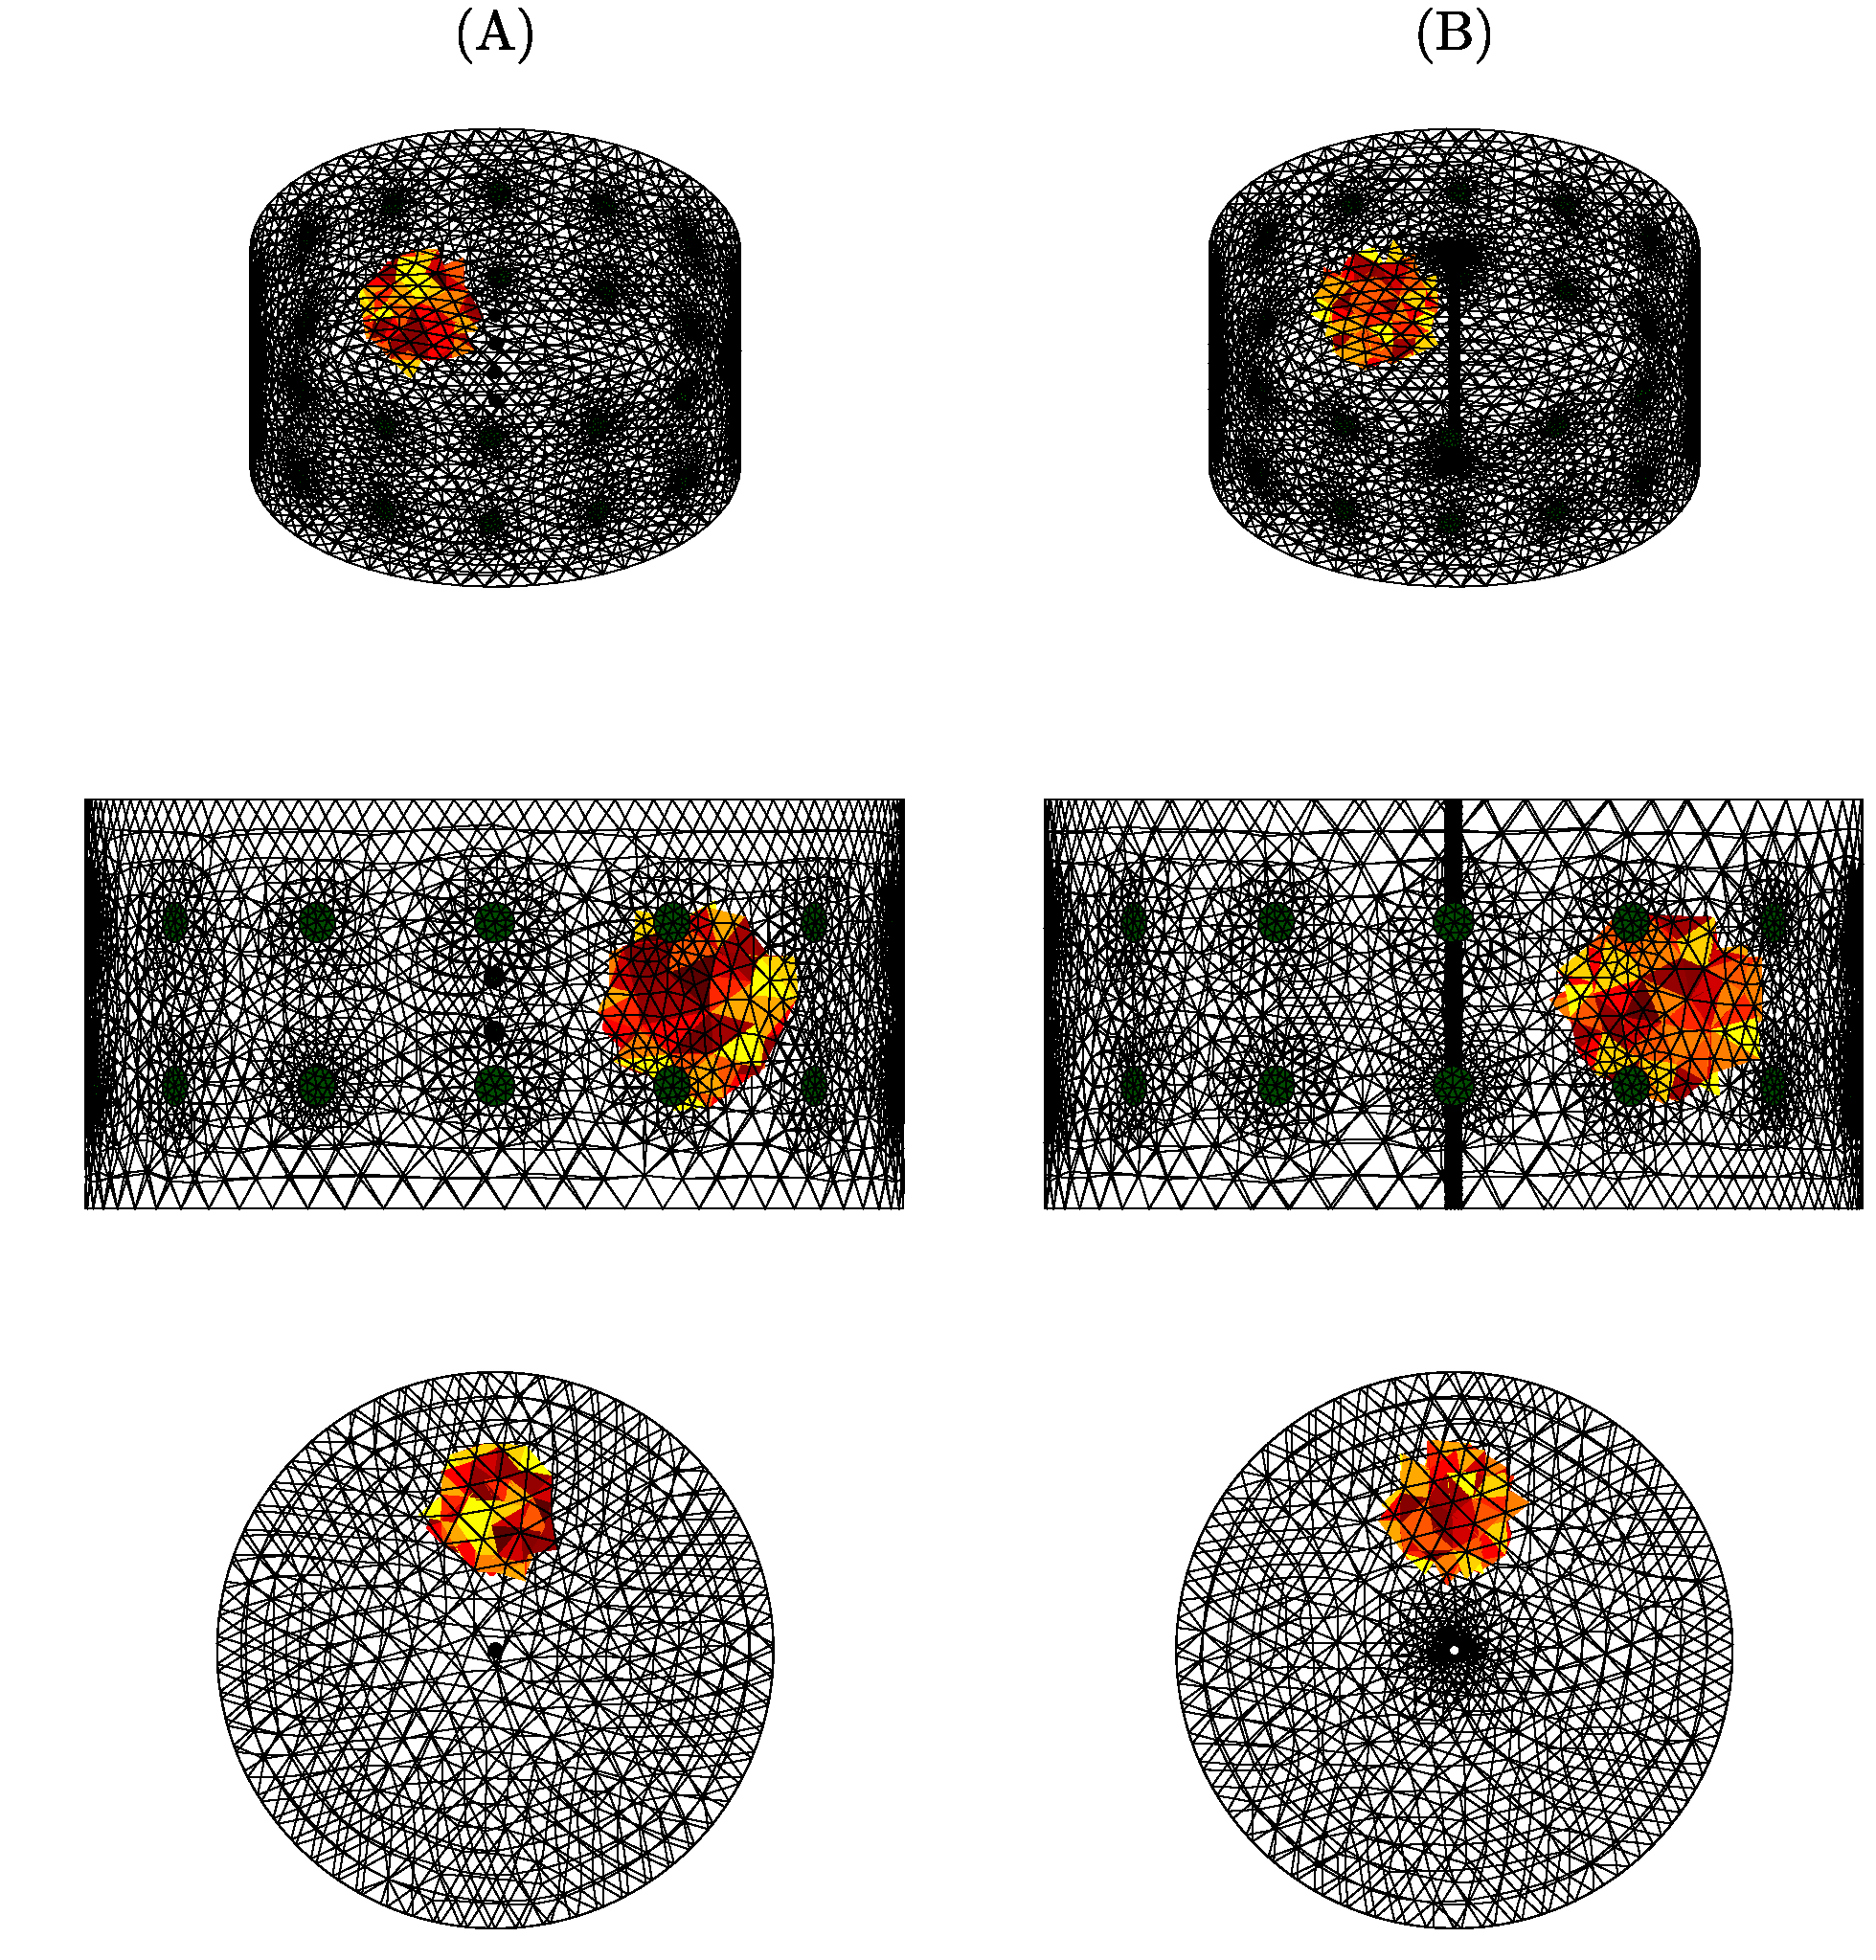
\includegraphics[width=0.52\textwidth,trim={18cm 0cm 0 1.4cm},clip]{probe_types.pdf}
			\end{figure}
		\end{column}
		\begin{column}{0.5\textwidth}
			\begin{itemize}
				\item High sensitivity near the internal probe
				\item A small amount of movement produces a large artefact
			\end{itemize}
		\end{column}
	\end{columns}%	
\end{frame}

\begin{frame}
	\frametitle{Chapter 7: Internal Electrode Motion}
	\framesubtitle{Methods}
	For a probe is moved 5\% of the tank radius: \\ \vspace{2mm}
	\begin{figure}[H]
		\centering
		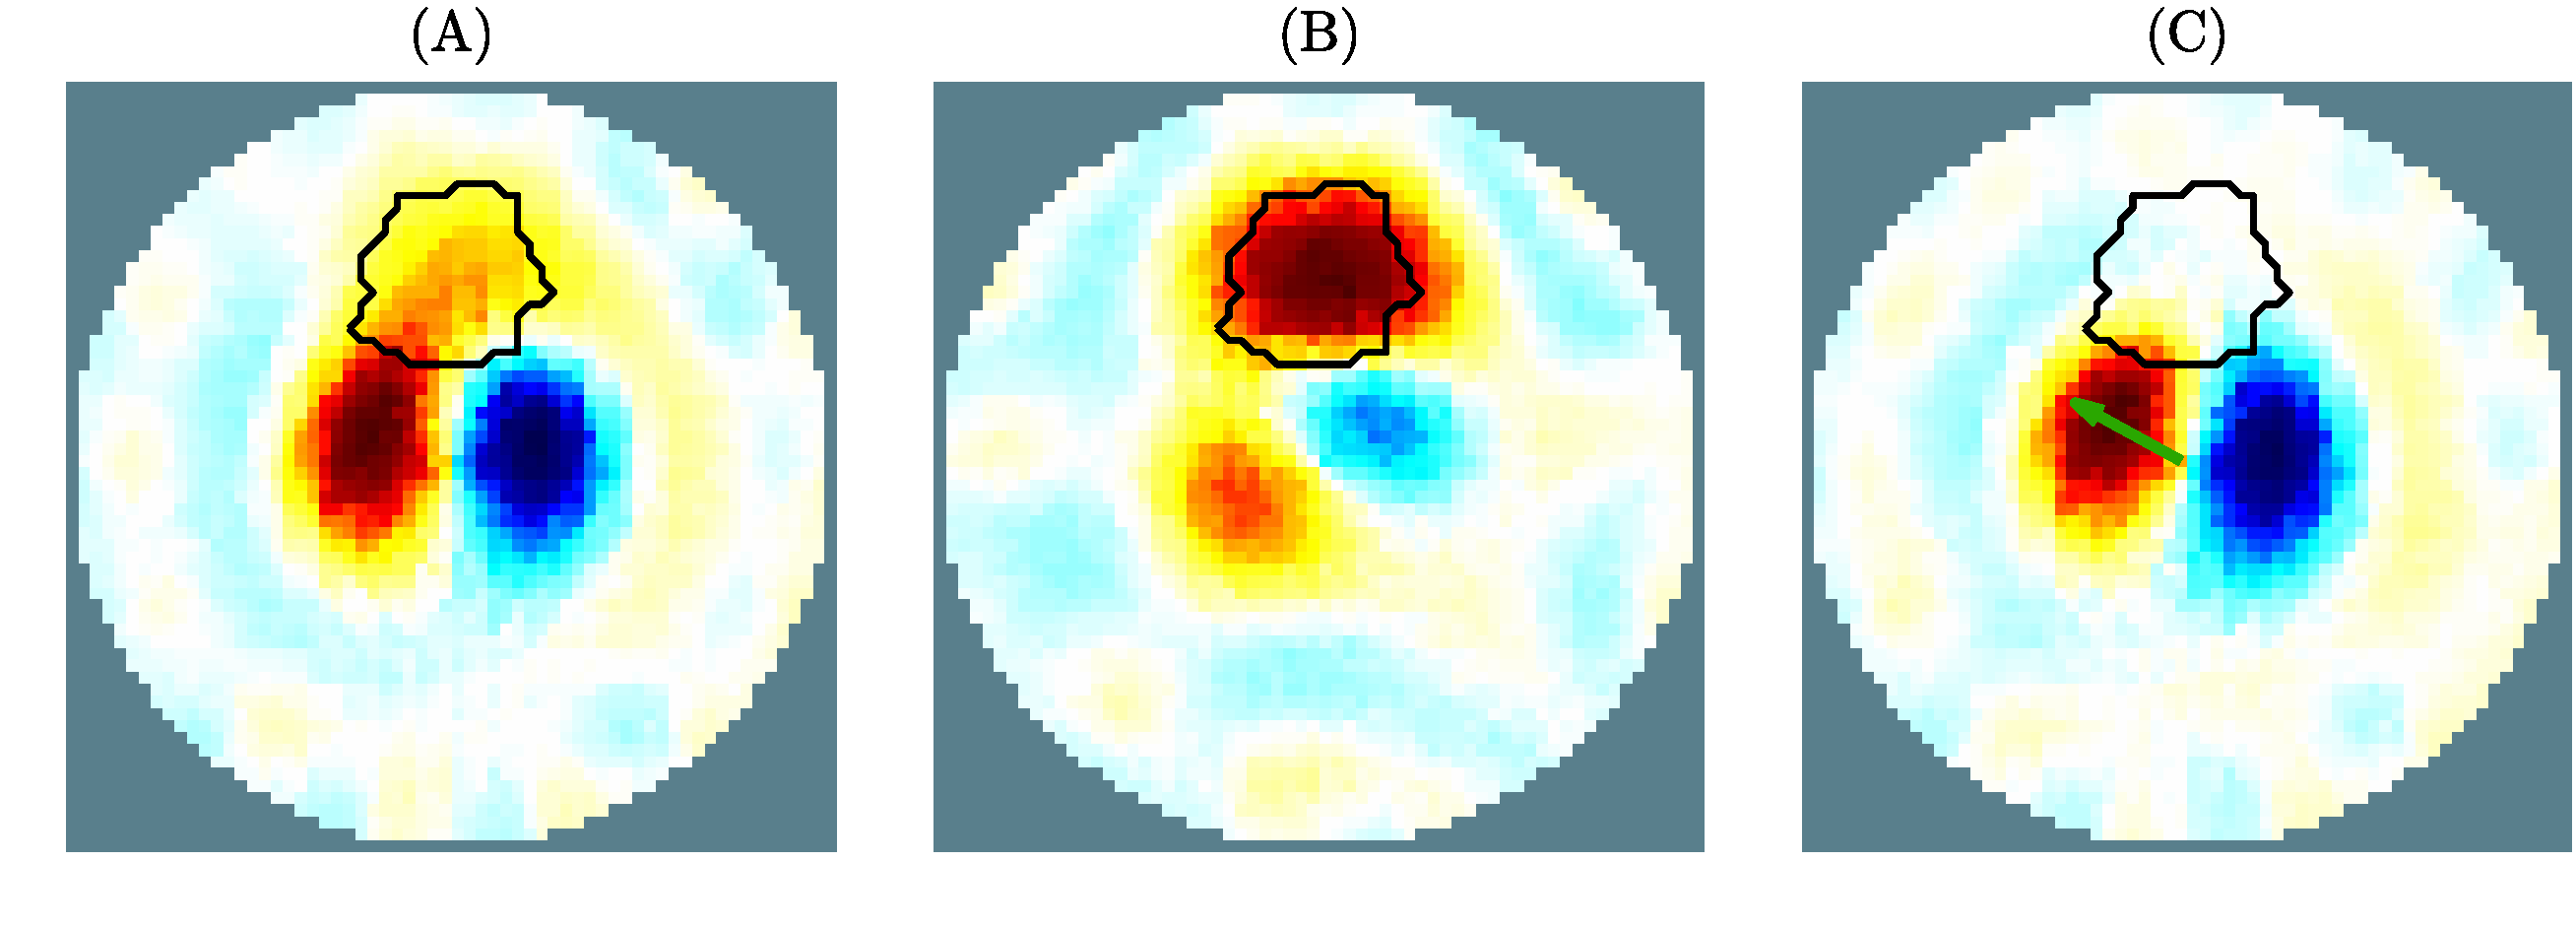
\includegraphics[width=\textwidth,trim={0cm 0.6cm 0 1.4cm},clip]{recon_methods.pdf}
	\end{figure}
	\begin{columns}[c]
		\begin{column}{0.33\textwidth}
			\centering
			{\large Regular reconstruction} 
		\end{column}
		\begin{column}{0.33\textwidth}
			\centering
			{\large Reconstruction with original motion correction} 
		\end{column}
		\begin{column}{0.33\textwidth}
			\centering
			{\large Reconstructing the effect of motion only}
		\end{column}
		\end{columns}
		\vspace{5mm}
		\centering
		\alert{This direction is used to generate a new model for reconstruction}
\end{frame}

\begin{frame}
	\frametitle{Chapter 7: Internal Electrode Motion}
	\framesubtitle{Results}
	\begin{columns}[c]
		\begin{column}{0.65\textwidth}
			\begin{figure}[H]
				\centering
				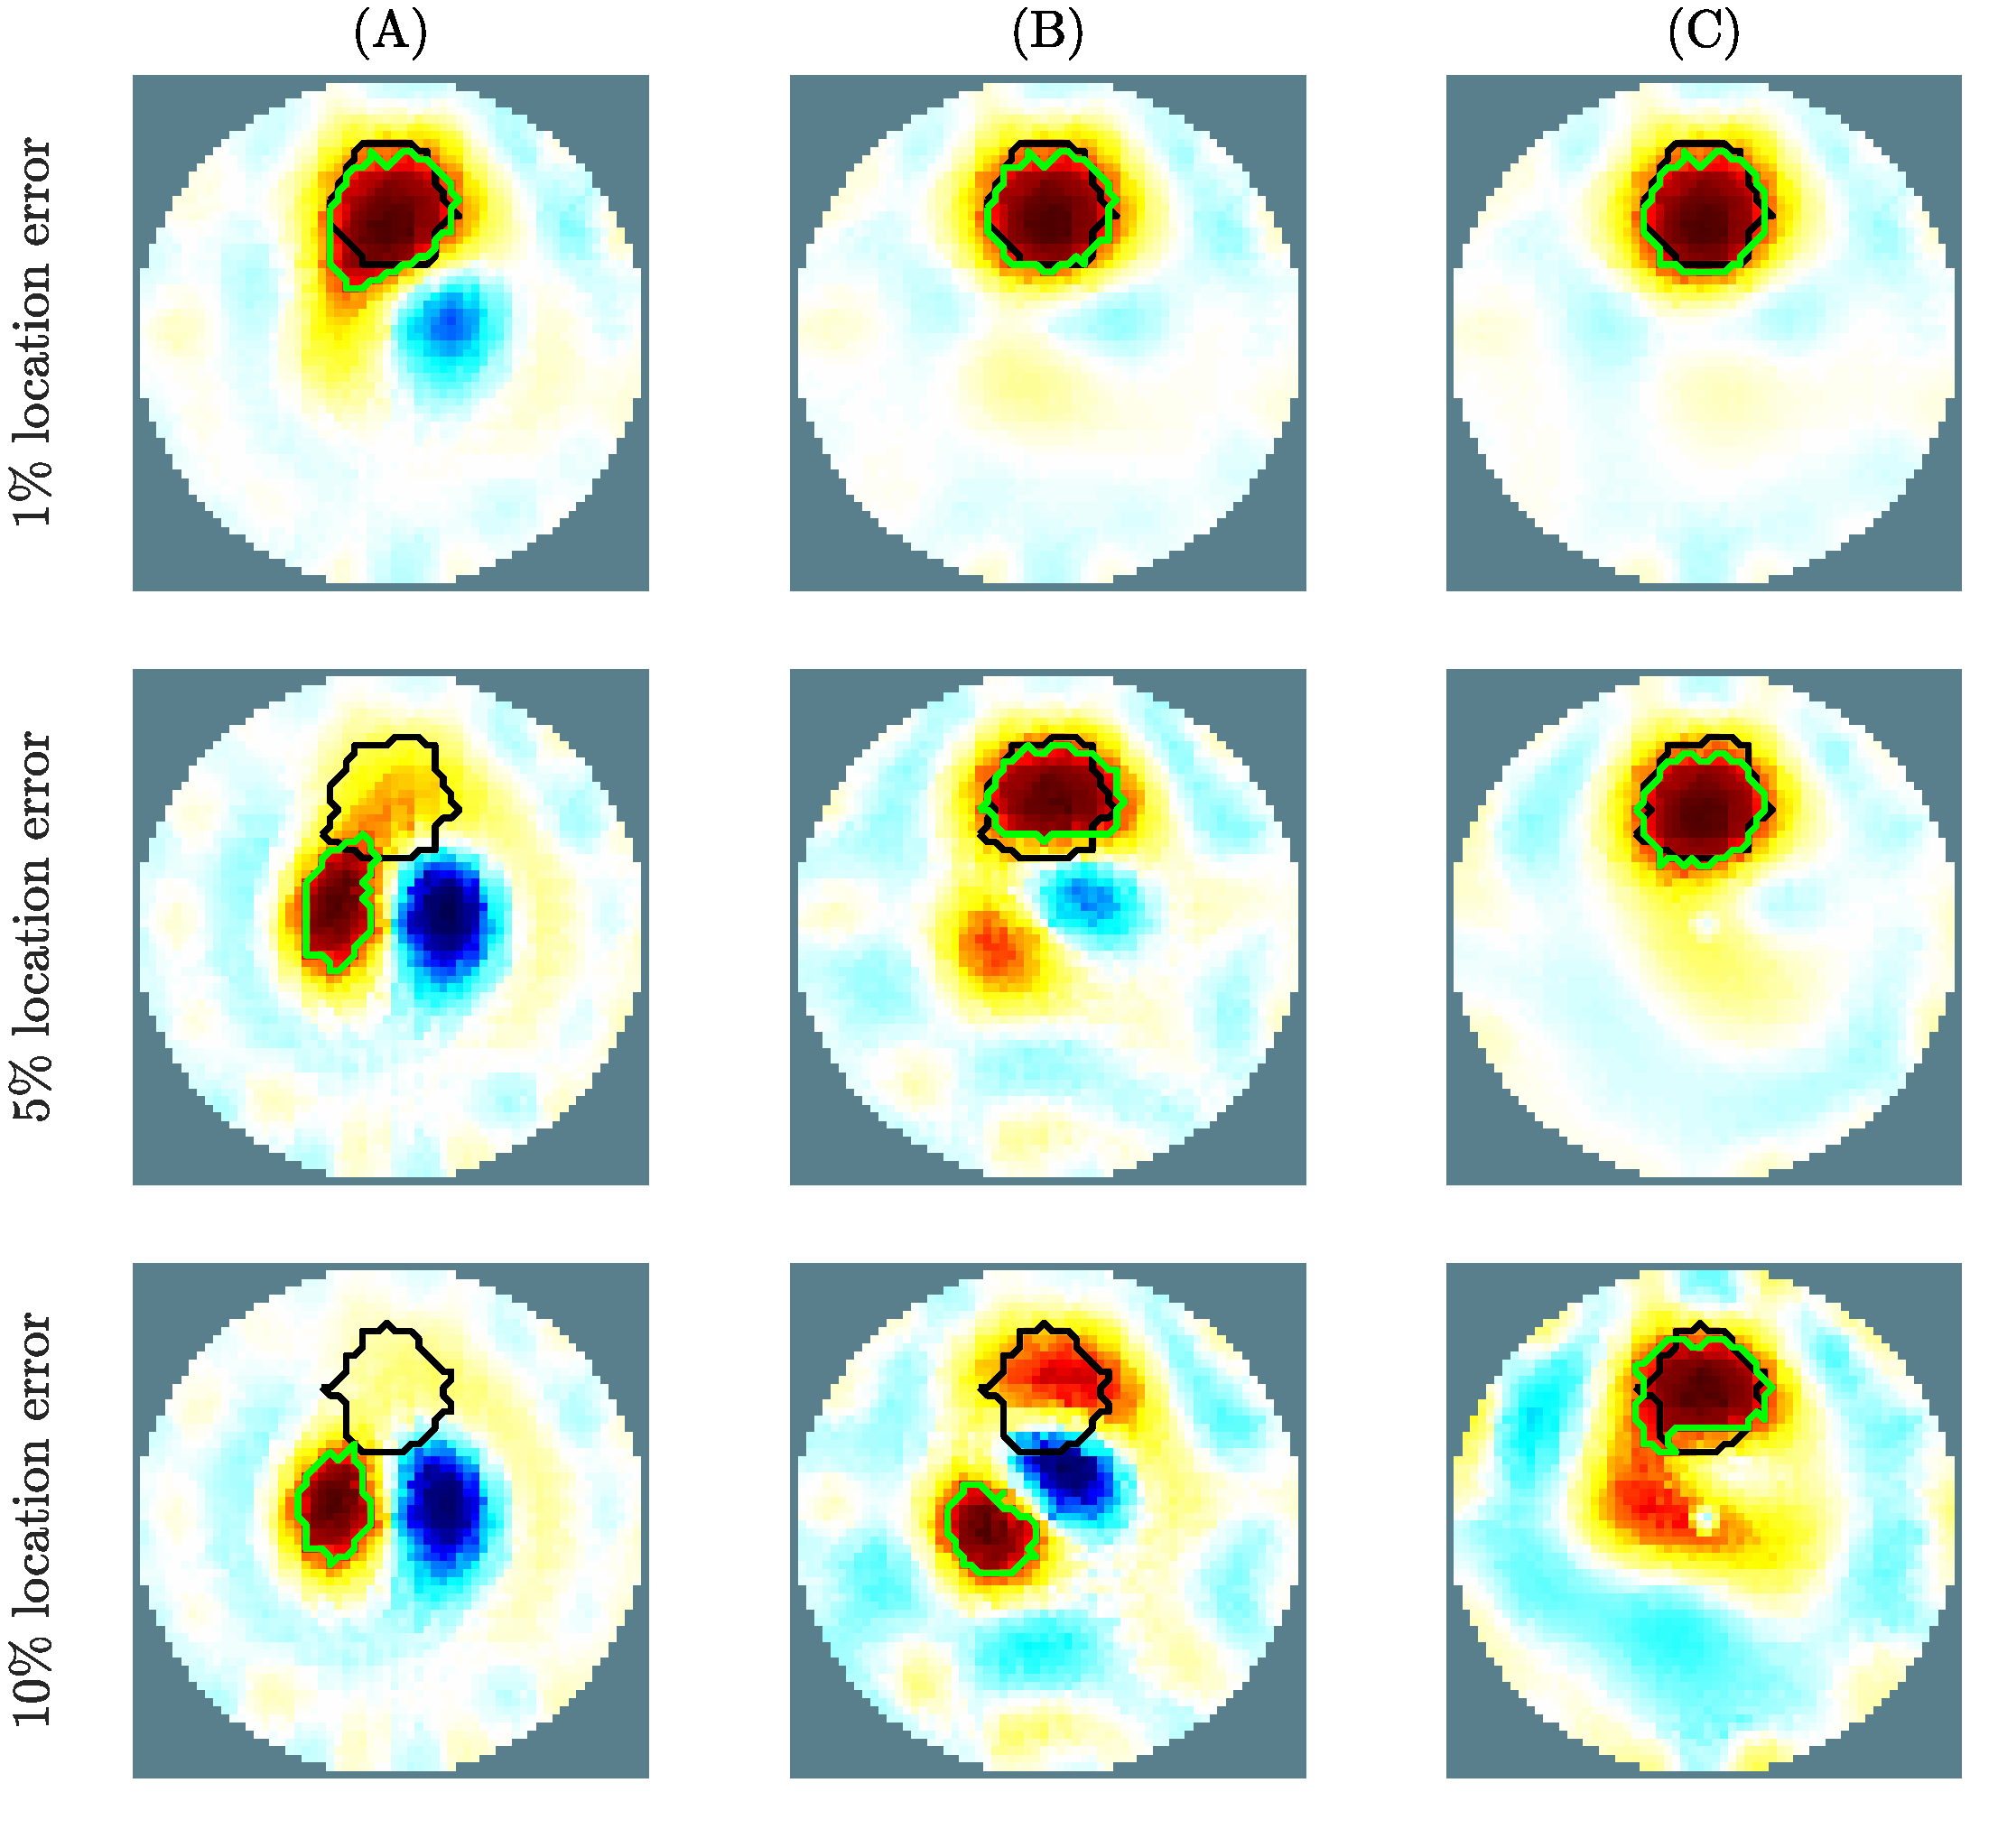
\includegraphics[width=0.95\textwidth,trim={0cm 0.6cm 0 0cm},clip]{recon_accuracy_hollow_loc_10.pdf}
			\end{figure}
		\end{column}
		\begin{column}{0.35\textwidth}
			\begin{itemize}
				\item \alert{\textbf{A}} -- No motion correction
				\vspace{4mm}
				\item \alert{\textbf{B}} -- Regular motion correction
				\vspace{4mm}
				\item \alert{\textbf{C}} -- Probe position correction
			\end{itemize}
			\vspace{10mm}
			Actual (black) vs. reconstructed ({\color{green} green}) target location.
		\end{column}
	\end{columns}
\end{frame}

\begin{frame}
	\frametitle{Chapter 7: Internal Electrode Motion}
	\framesubtitle{Results}
			\begin{figure}[H]
				\centering
				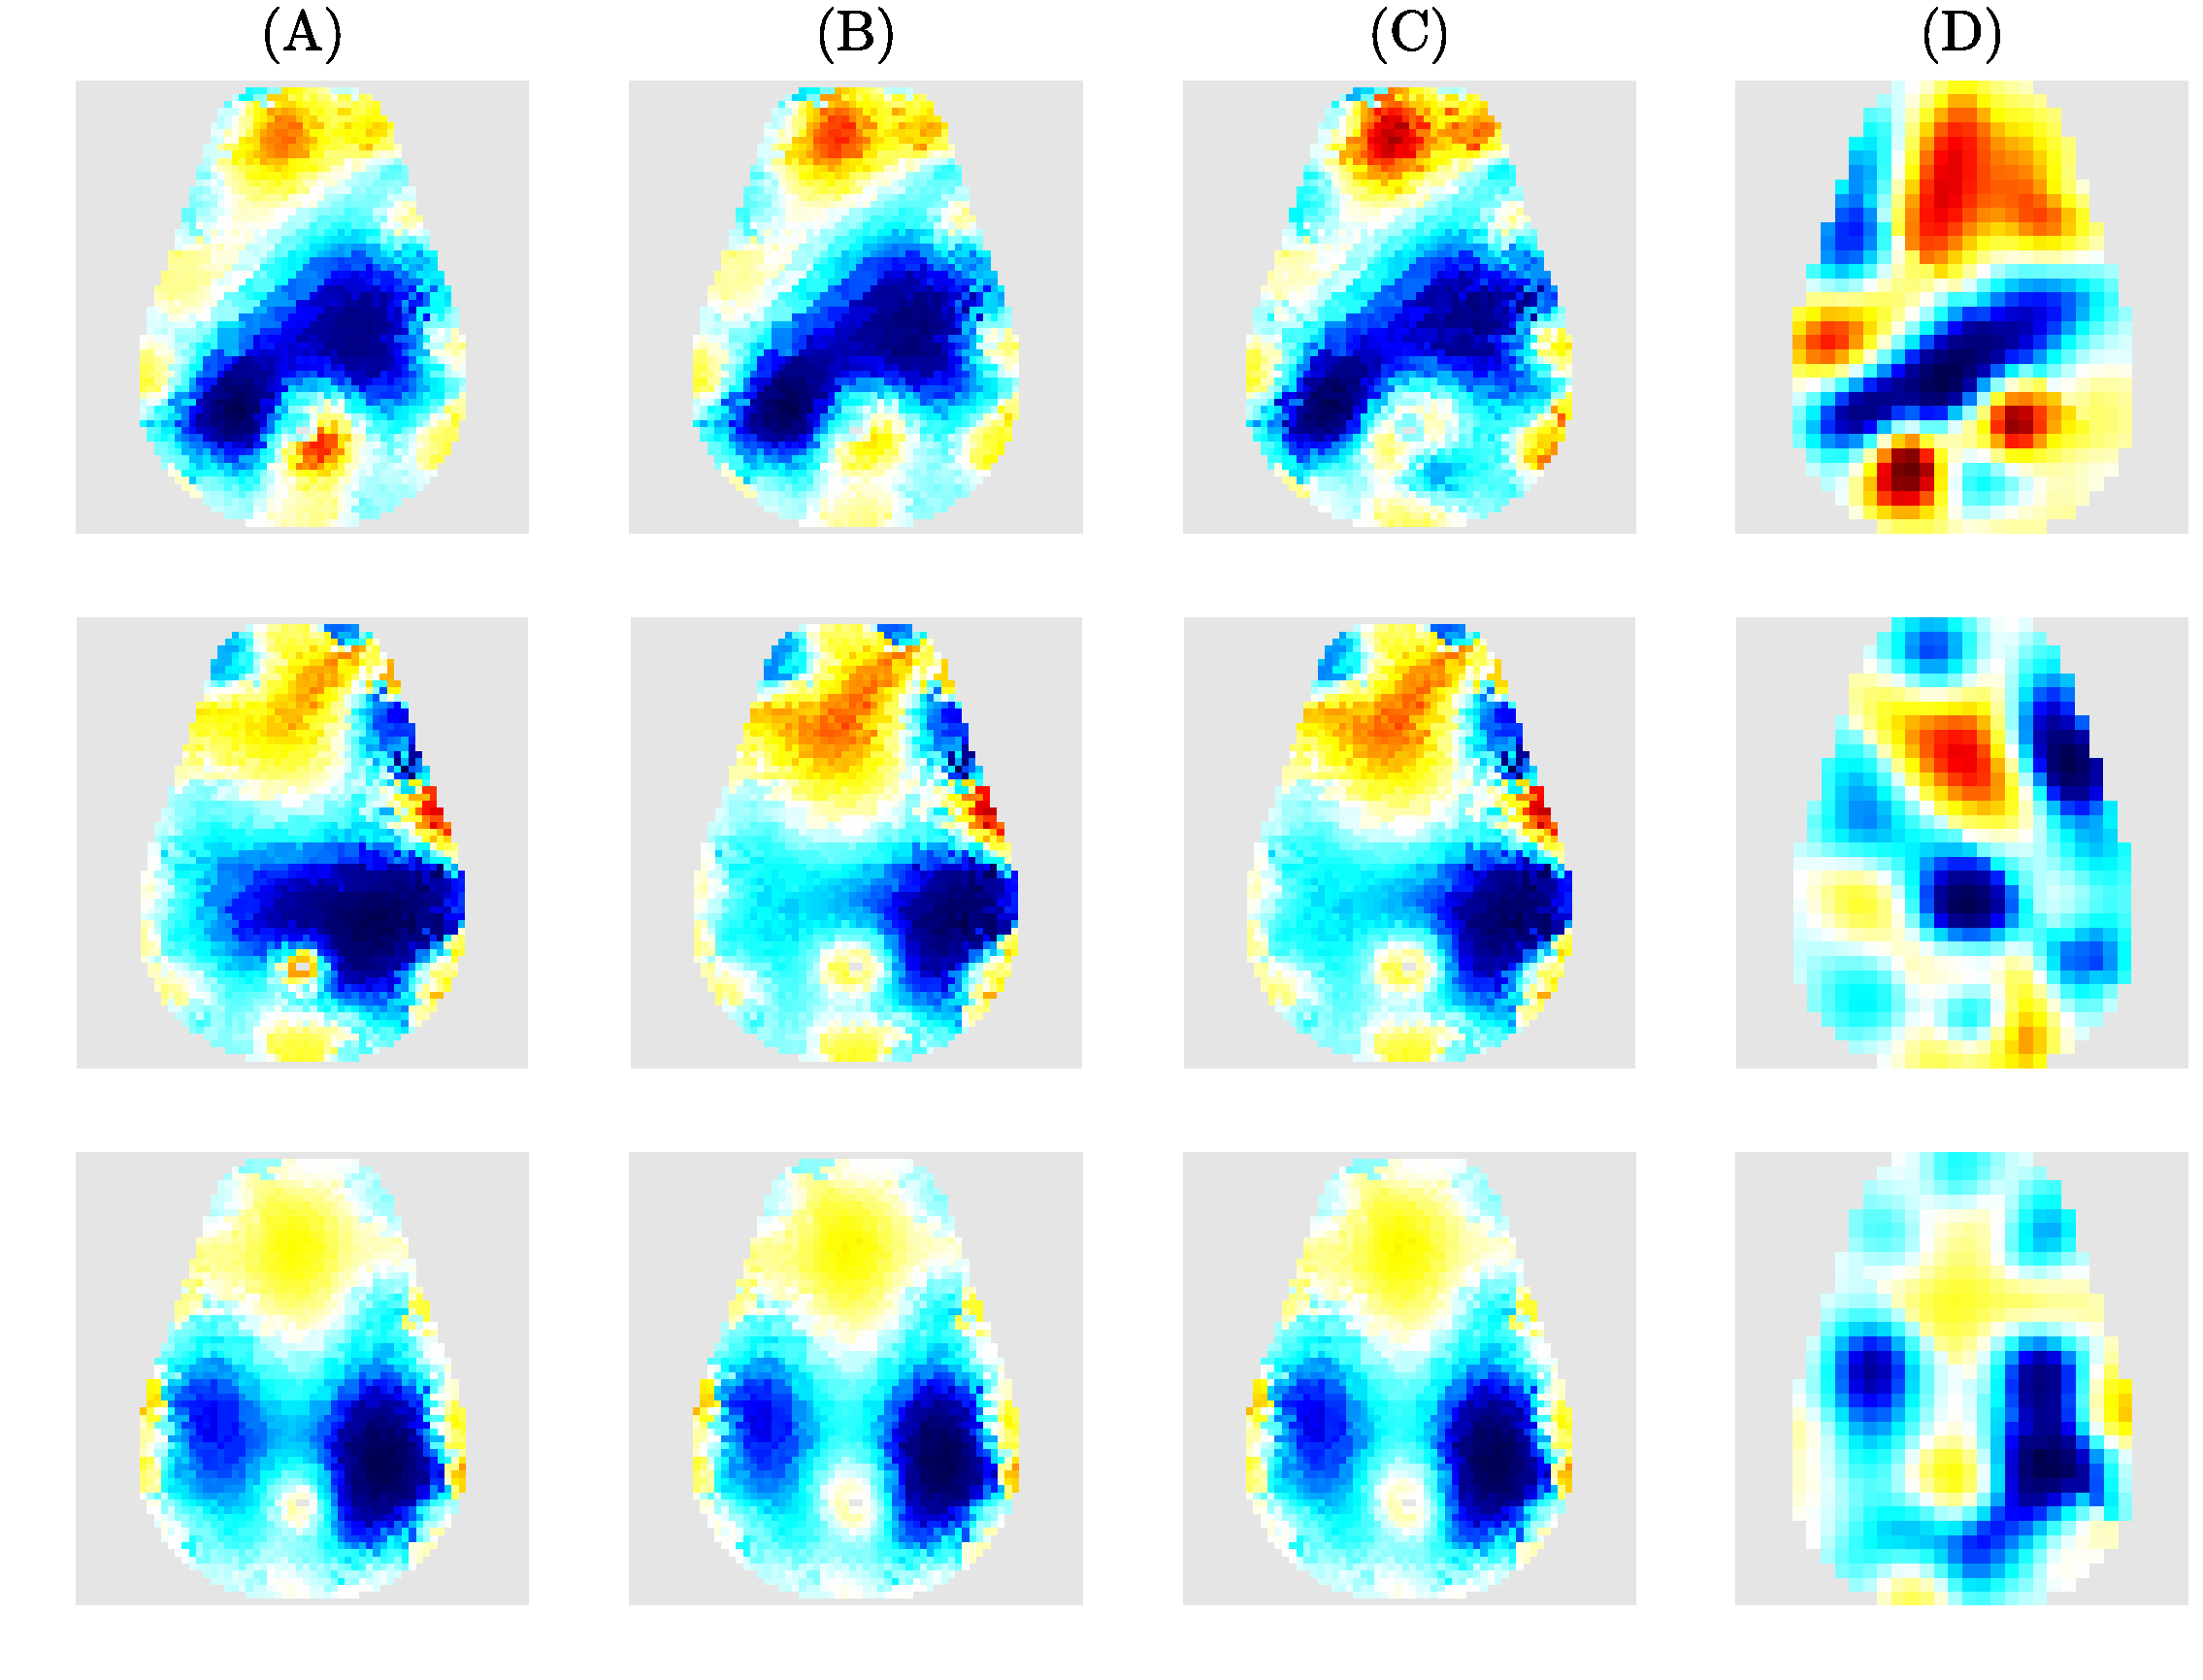
\includegraphics[width=\textwidth,trim={0cm 0cm 10cm 20cm},clip]{lamb_reconstruction_all.pdf}
			\end{figure}
			Increased separability of the lungs with regular motion correction (column 2) and 
			probe position correction (column 3)
\end{frame}

\begin{frame}
	\frametitle{Chapter 7: Internal Electrode Motion}
	\framesubtitle{Results}
	\begin{columns}[c]
		\begin{column}{0.25\textwidth}
			\begin{figure}[H]
				\centering
				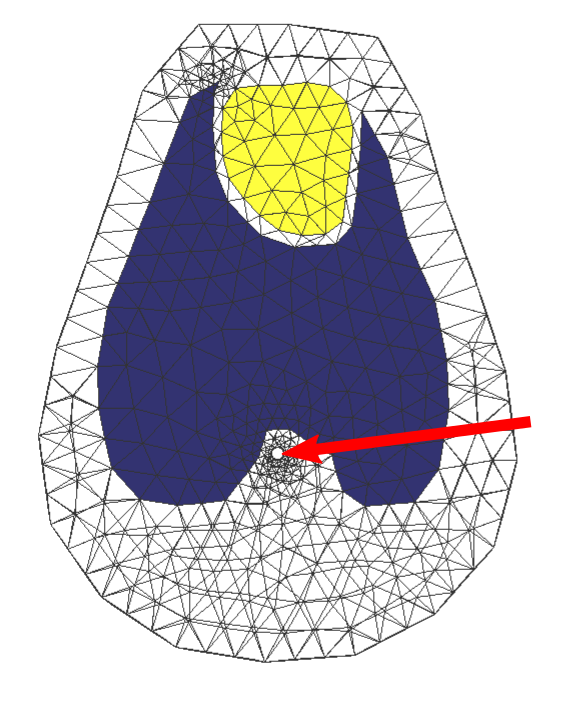
\includegraphics[width=\textwidth,trim={0cm 0.6cm 0 0cm},clip]{internal_probe_location.png}
			\end{figure}
		\end{column}
		\begin{column}{0.75\textwidth}
			\begin{figure}[H]
				\centering
				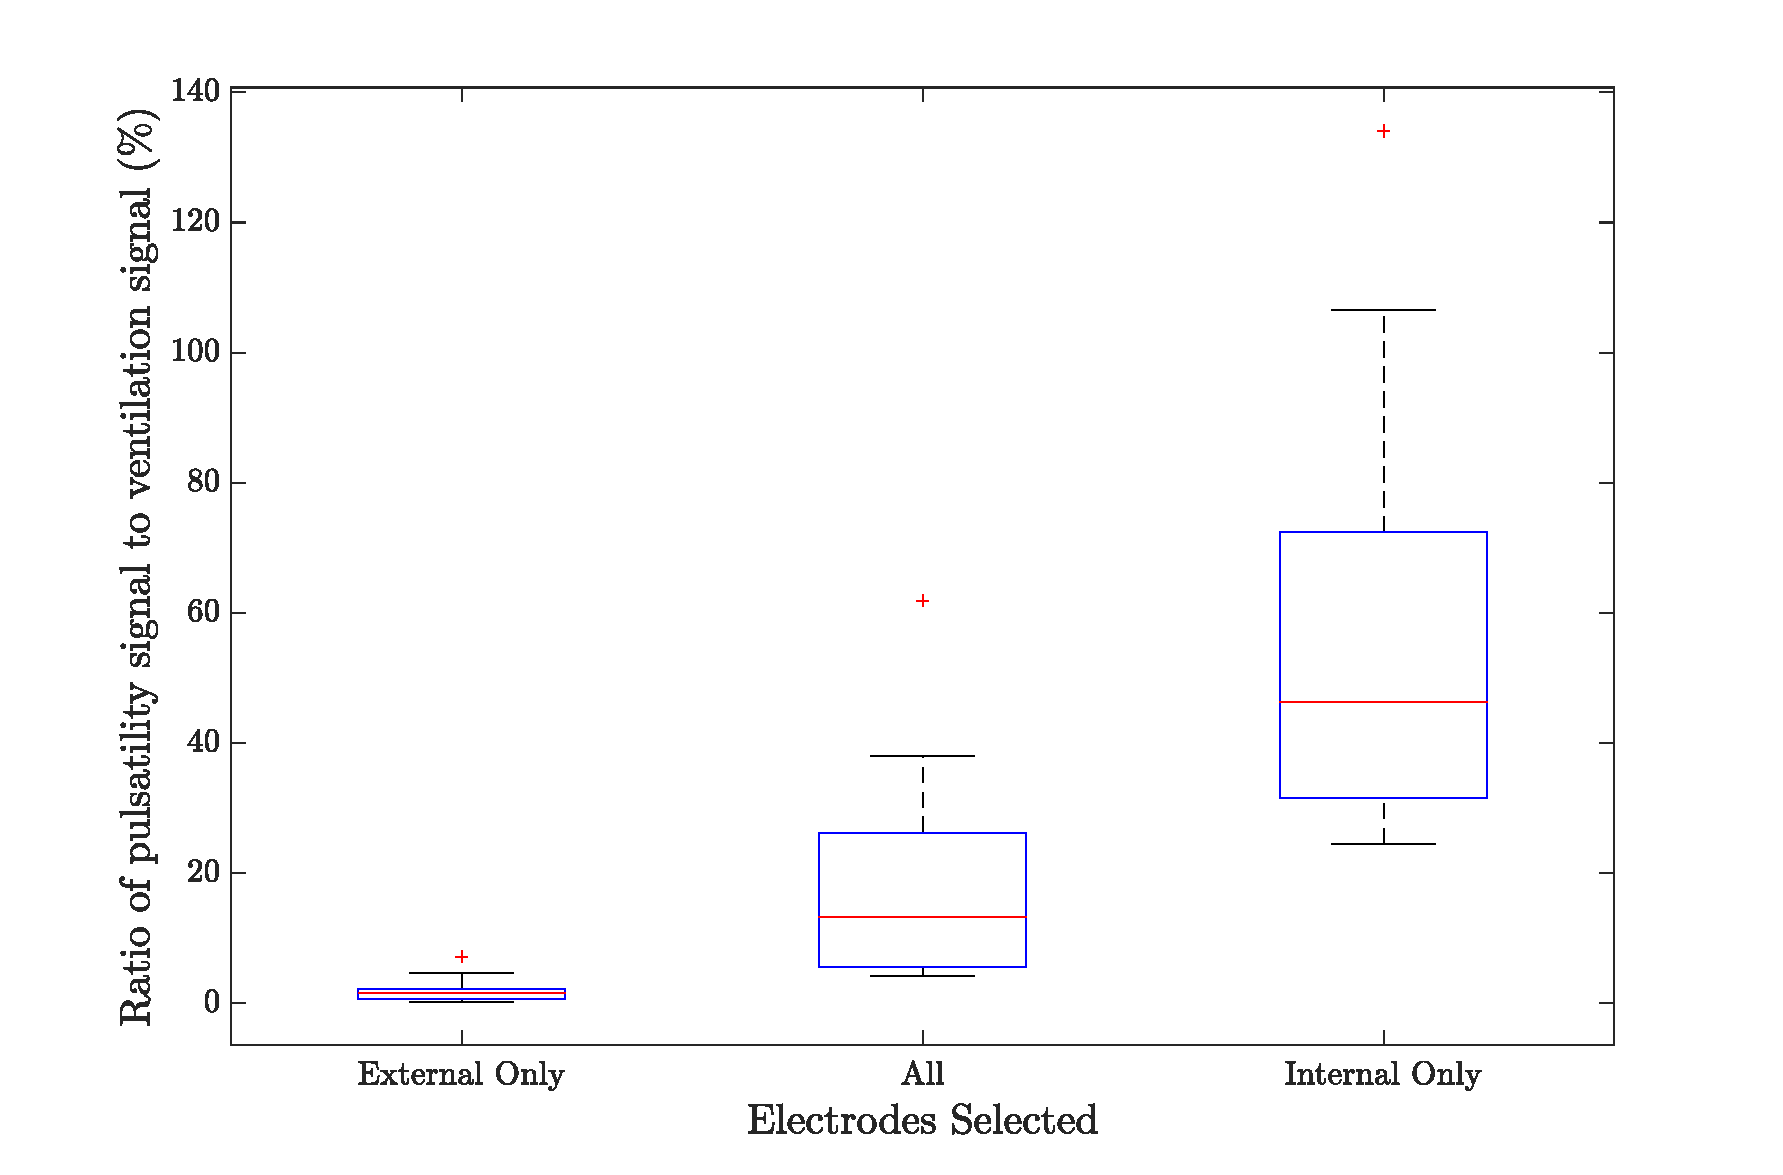
\includegraphics[width=0.95\textwidth,trim={0cm 0.6cm 0 0cm},clip]{amplitude_ratio.pdf}
			\end{figure}
		\end{column}
	\end{columns}
\end{frame}

\begin{frame}
\frametitle{Conclusion}
\framesubtitle{Summary}
\textbf{This thesis presents:}
\vspace{2mm}
\begin{itemize}
	\item Potential for filtering based measures of perfusion imaging
	\begin{itemize}
		\item limited sensitivity to cardiac frequency
		\item challenging to identify the lung regions
	\end{itemize}
	\vspace{2mm}
	\item Advanced modelling techniques to improve ventilation and lung localization

	\vspace{2mm}
	\item A reconstruction technique used \emph{in-vivo} that was able to correct for
	probe motion 
	\begin{itemize}
		\item Motion up to 5\% of the tank radius in simulation
	\end{itemize}
\end{itemize}
%\begin{columns}[c]
%	\begin{column}{0.5\textwidth}
%		\textbf{Challenges}
%		\vspace{2mm}
%		\begin{itemize}
%			\item Challenging to isolate perfusion in the lung regions 
%			\vspace{2mm}
%			\item Low sensitivity to cardiac-frequency impedance changes
%			\vspace{2mm}
%			\item Reconstructions with internal electrodes are challenging...
%		\end{itemize}
%	\end{column}
%	\begin{column}{0.5\textwidth}
%		\textbf{Contributions}
%			\vspace{2mm}
%		\begin{itemize}
%			\item Technique to improve identification of boundary and lung regions
%			\vspace{2mm}
%			\item Internal electrodes to increase internal sensitivity
%			\vspace{2mm}
%			\item Correct for movement of internal electrodes
%		\end{itemize}
%	\end{column}
%\end{columns}
\end{frame}

\begin{frame}
\frametitle{Conclusion}
\framesubtitle{Future Work}
\begin{enumerate}
	\item Collect data from a range of patients to test automatic segmentation software
	\vspace{3mm}
	\item Meshing tool to control mesh dissipation on complex geometry 
	\vspace{3mm}
	\item Validation of the safety of internal electrodes for clinical use
	\vspace{3mm}
	\item Incorporate internal electrode reconstruction into standard reconstruction algorithms (GREIT)
\end{enumerate}

\end{frame}

\begin{frame}
  \titlepage
\end{frame}

%%%%%%%%%%%%%%%%%%%%%%%%%%%%%%%%%%%%%%%%%%%%%%%%%%%%%%%%%%%%%%%
\end{document}
